%\clearpage
\label{W+jets_control_region_bg}

Figures~\ref{fig:CRWjetResLoosePlots1Lep}, \ref{fig:CRWjetResLoosePlots1Lep2}, \ref{fig:CRWjetResTightPlots1Lep}, \ref{fig:CRWjetResTightPlots1Lep2}, \ref{fig:CRWjetMerPlots1Lep}, and \ref{fig:CRWjetMerPlots1Lep2} show the main relevant kinematic variable distributions in the \Wjets CRs for the \olep\ channel, after \mjjtag\ reweighting has been applied.
The definitions of these CRs are provided in Section~\ref{wcr_definition}. It is worth noting that the resolved loose \Wjets control region is utilized solely to study and validate the agreement between the data and MC samples and is not included in the inputs for the statistical analysis.


\begin{figure}[ht]
    \centering
    \subfloat[]{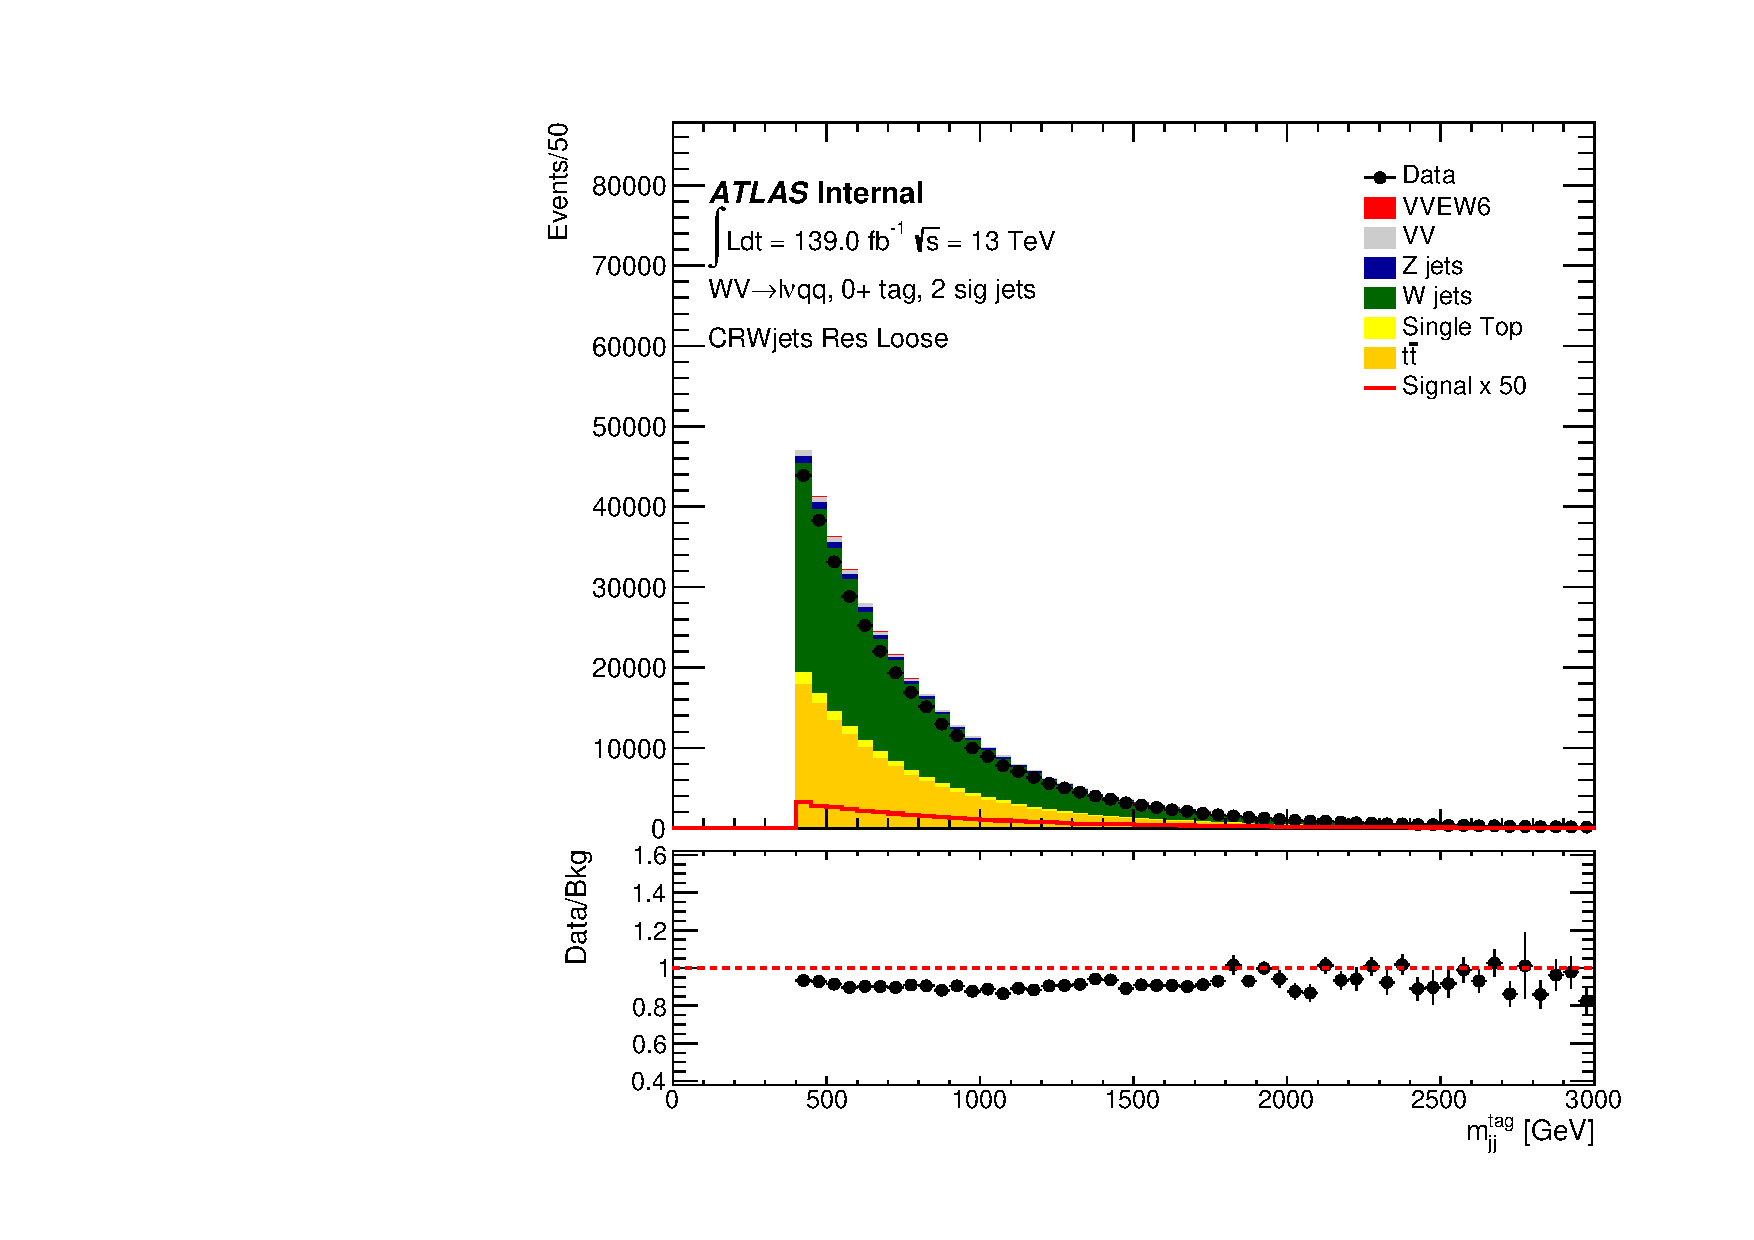
\includegraphics[width=0.3\textwidth]{figures/CRPlots/CRWjets_Res_Loose/stacked_plot_resolved_tagMjj.pdf}}
    \subfloat[]{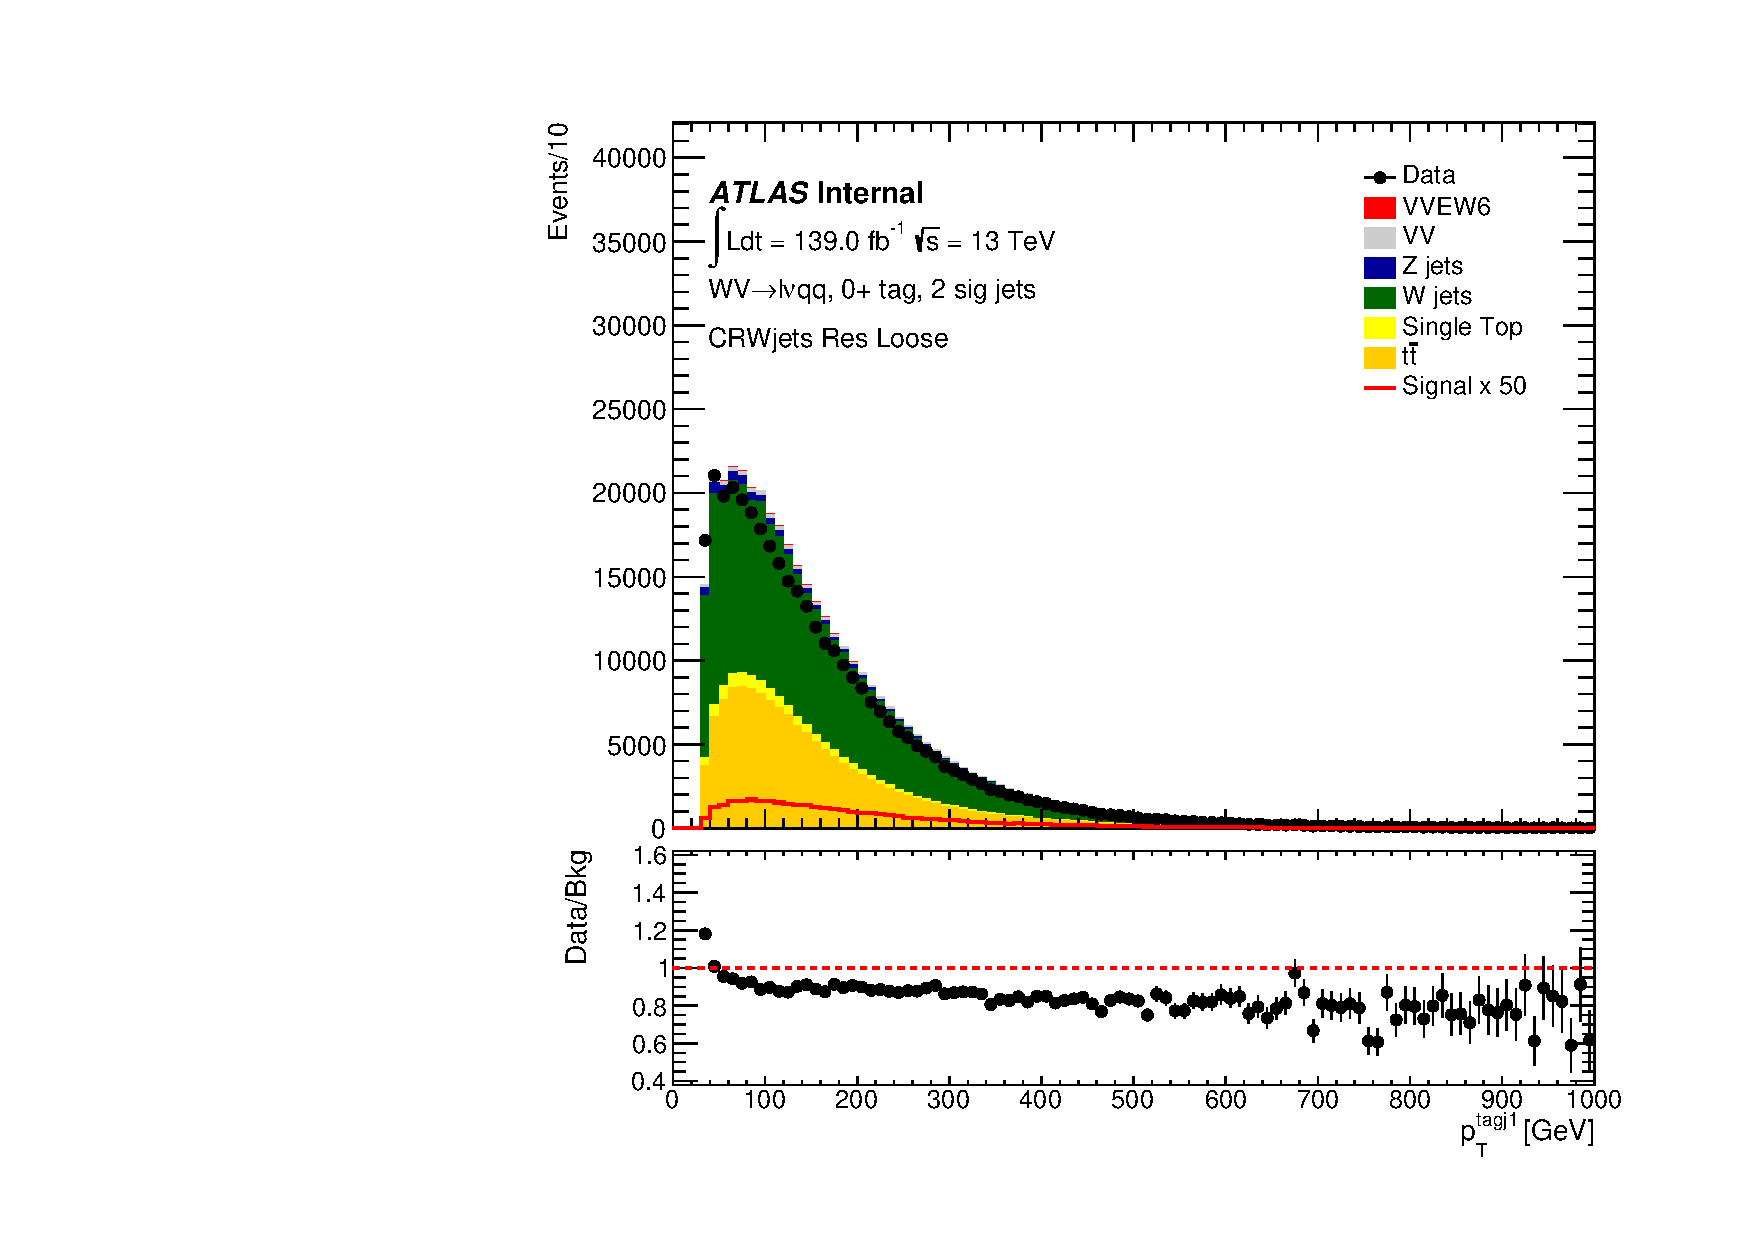
\includegraphics[width=0.3\textwidth]{figures/CRPlots/CRWjets_Res_Loose/stacked_plot_resolved_tagJ1_pt.pdf}}
    \subfloat[]{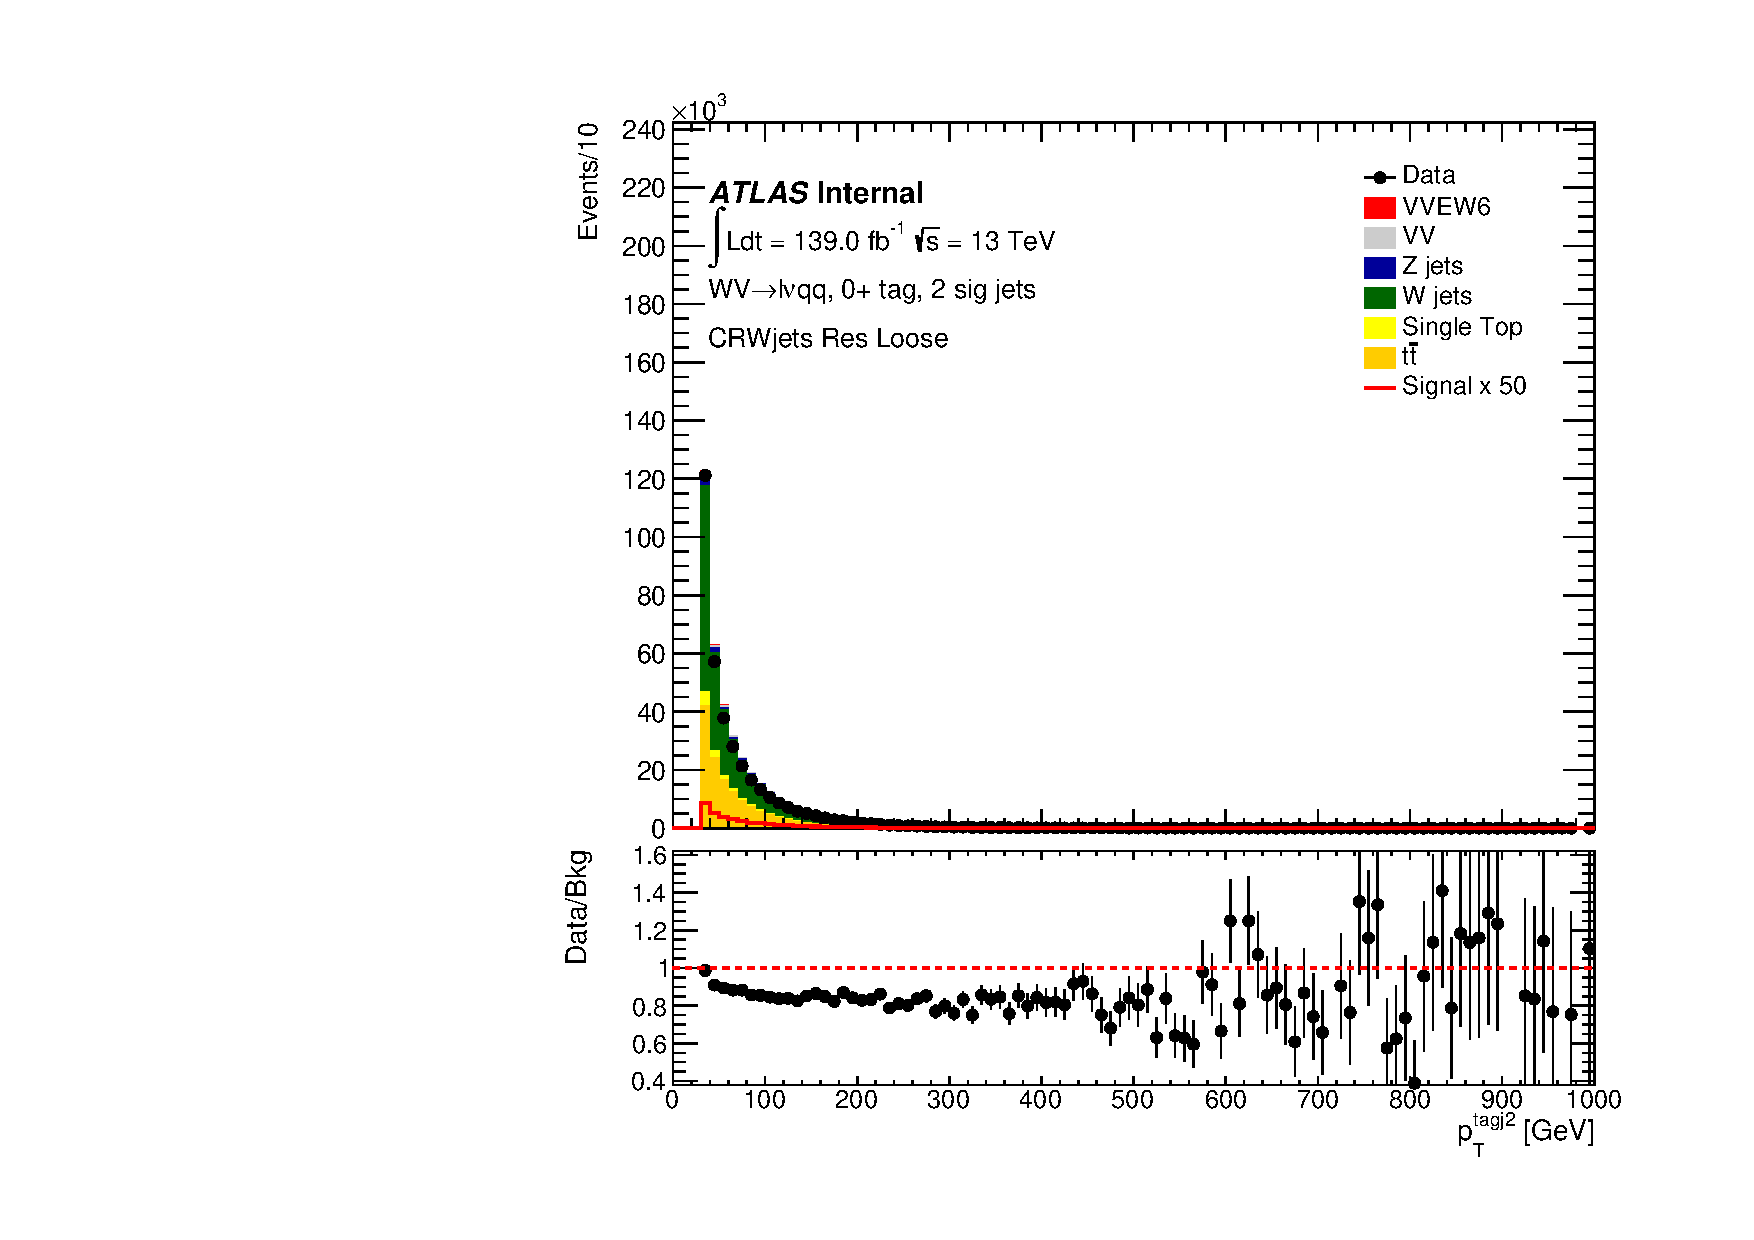
\includegraphics[width=0.3\textwidth]{figures/CRPlots/CRWjets_Res_Loose/stacked_plot_resolved_tagJ2_pt.pdf}} \\
    \subfloat[]{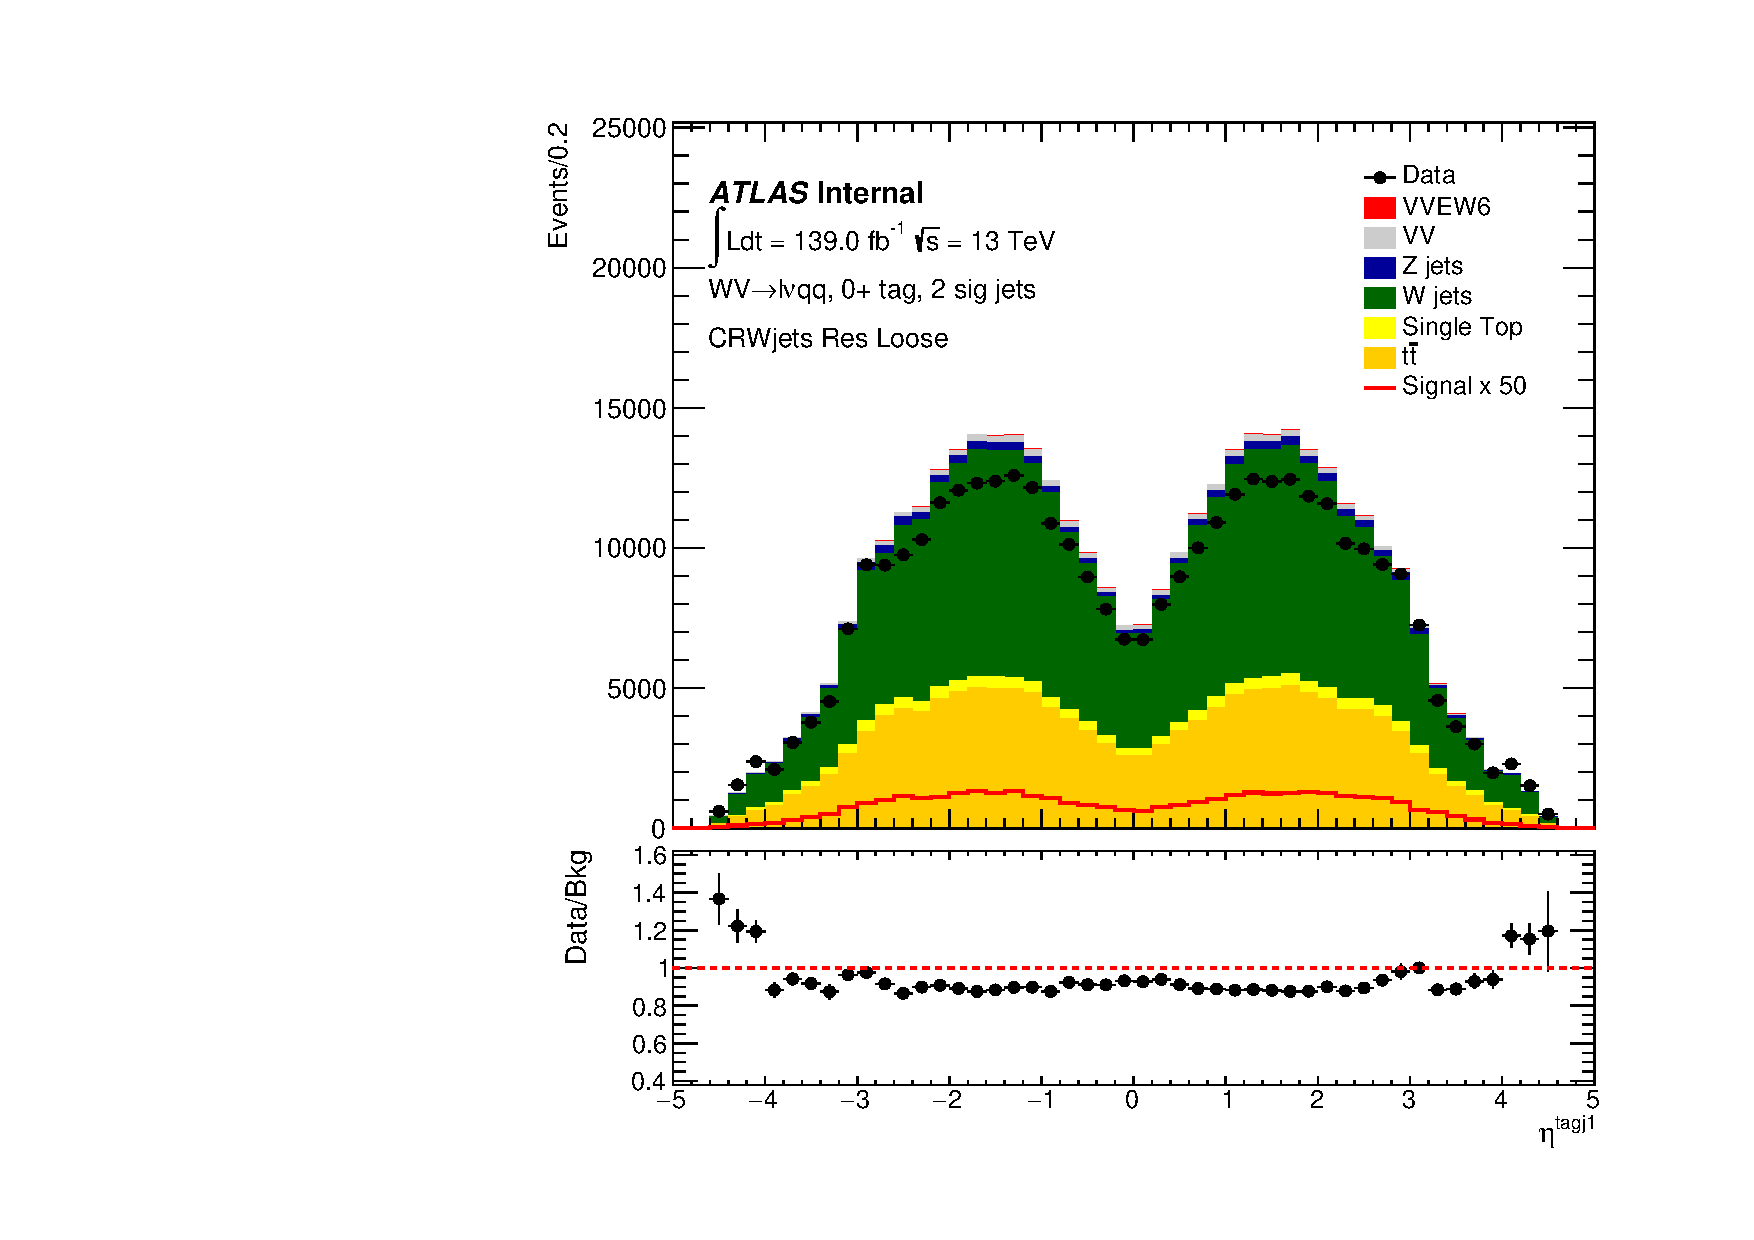
\includegraphics[width=0.3\textwidth]{figures/CRPlots/CRWjets_Res_Loose/stacked_plot_resolved_tagJ1_eta.pdf}}
    \subfloat[]{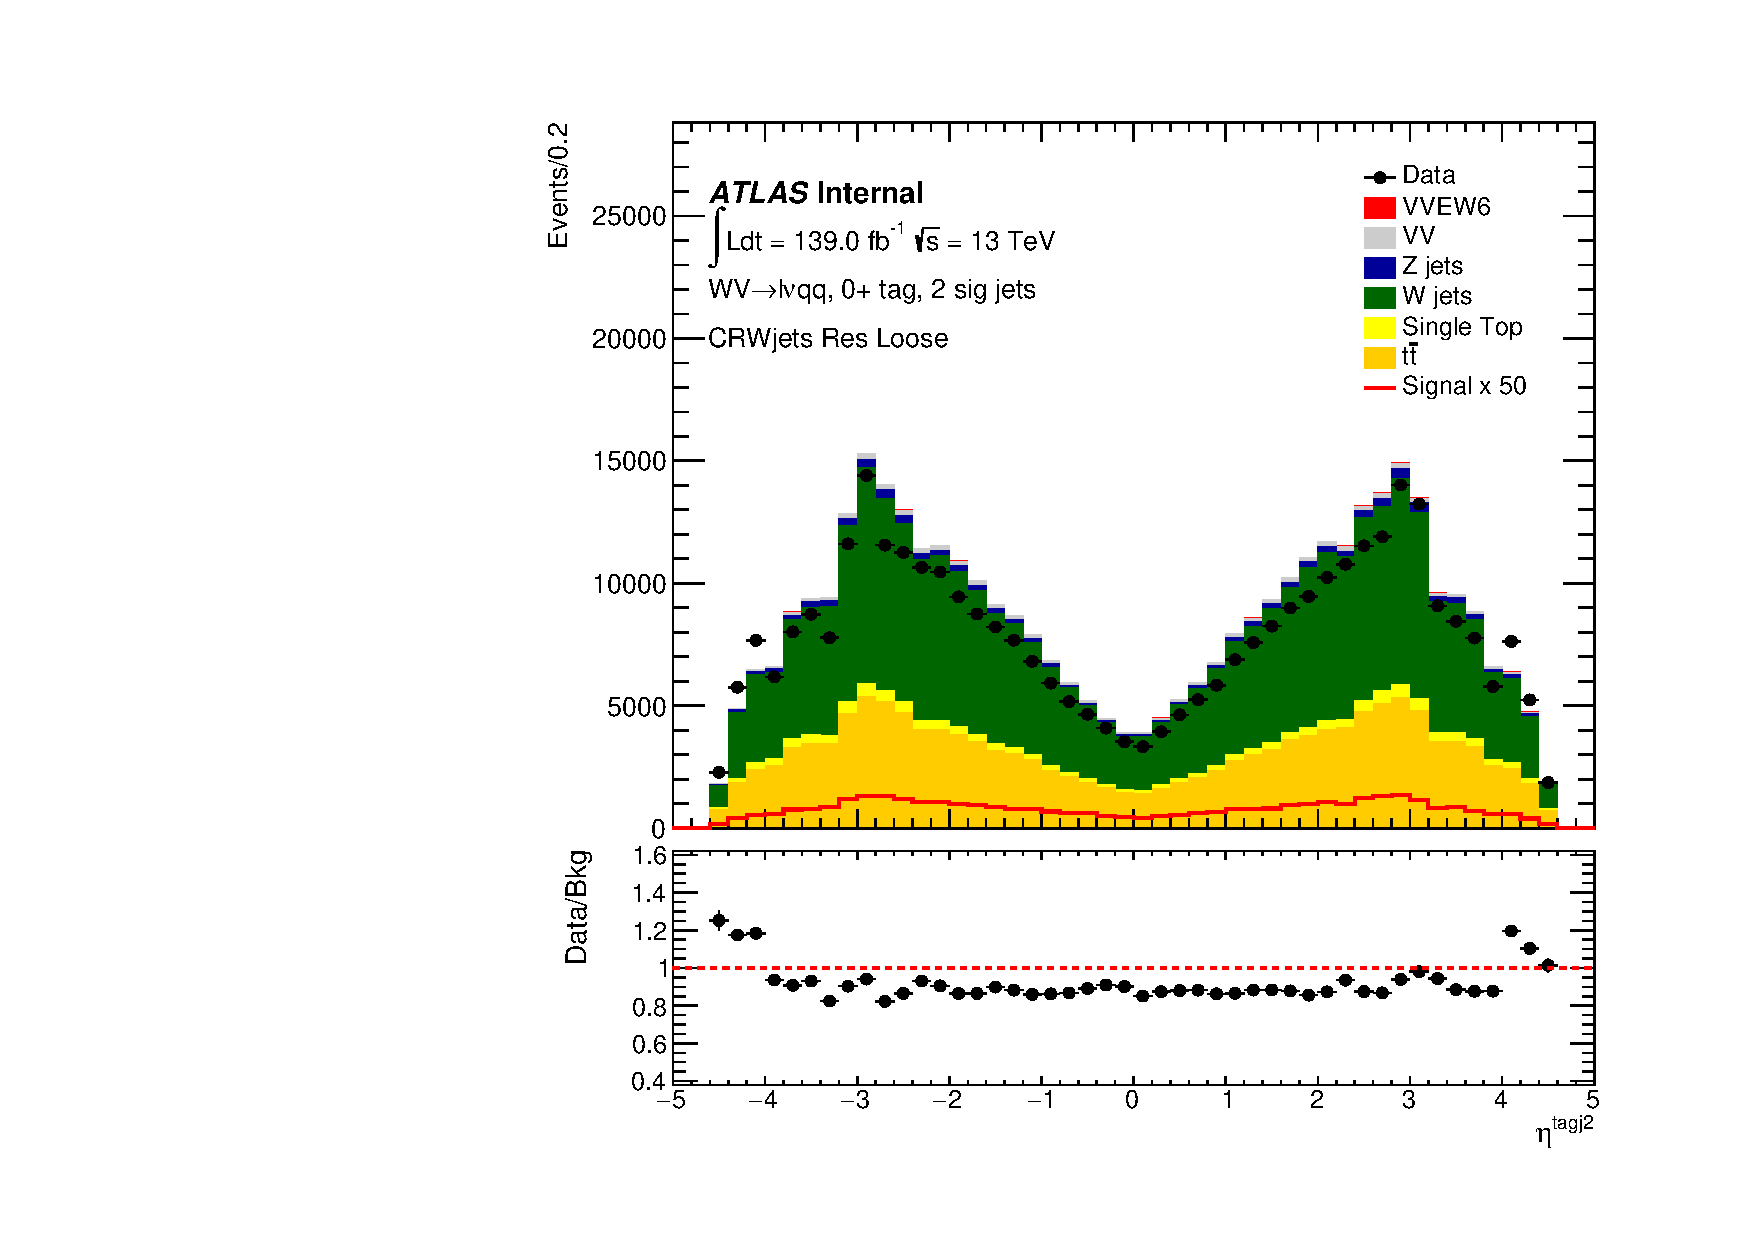
\includegraphics[width=0.3\textwidth]{figures/CRPlots/CRWjets_Res_Loose/stacked_plot_resolved_tagJ2_eta.pdf}} \\
    \subfloat[]{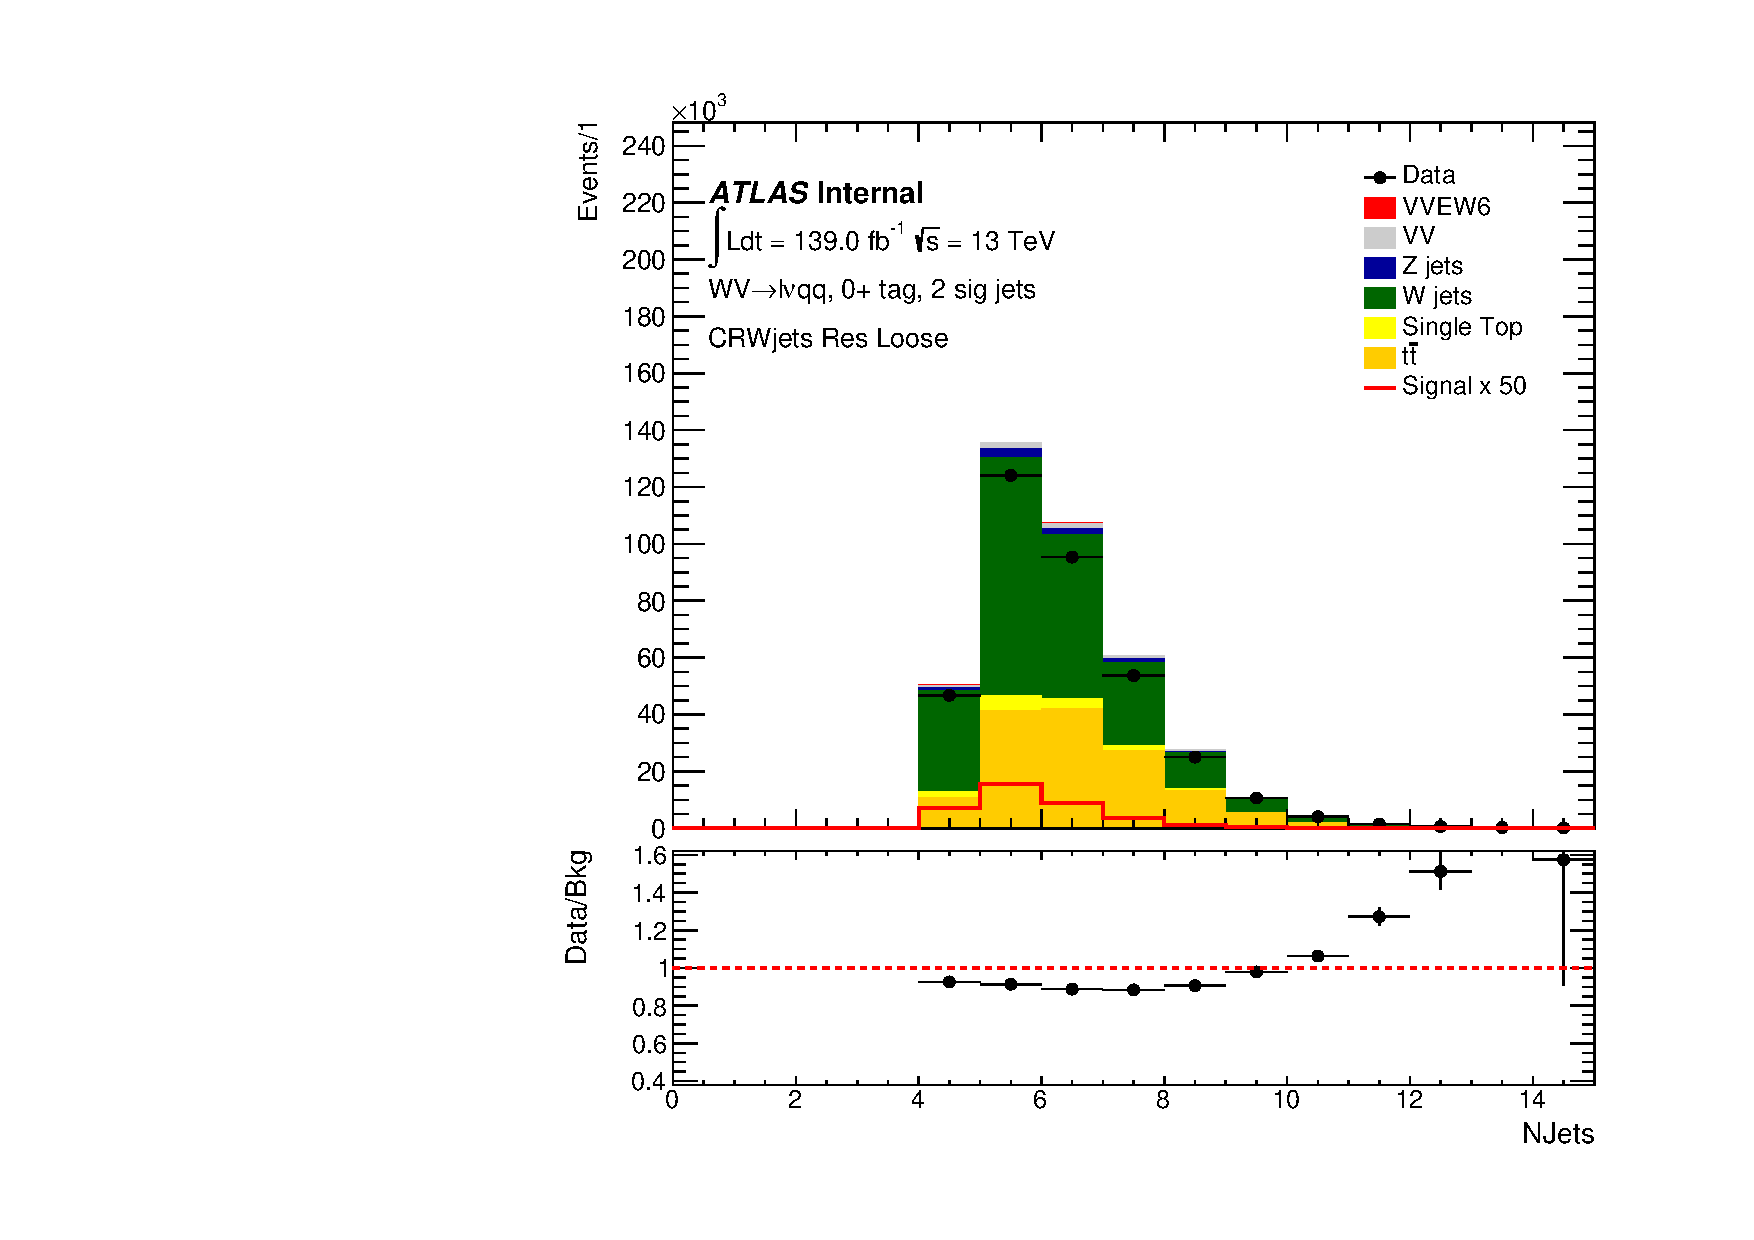
\includegraphics[width=0.3\textwidth]{figures/CRPlots/CRWjets_Res_Loose/stacked_plot_NJets.pdf}}
    \subfloat[]{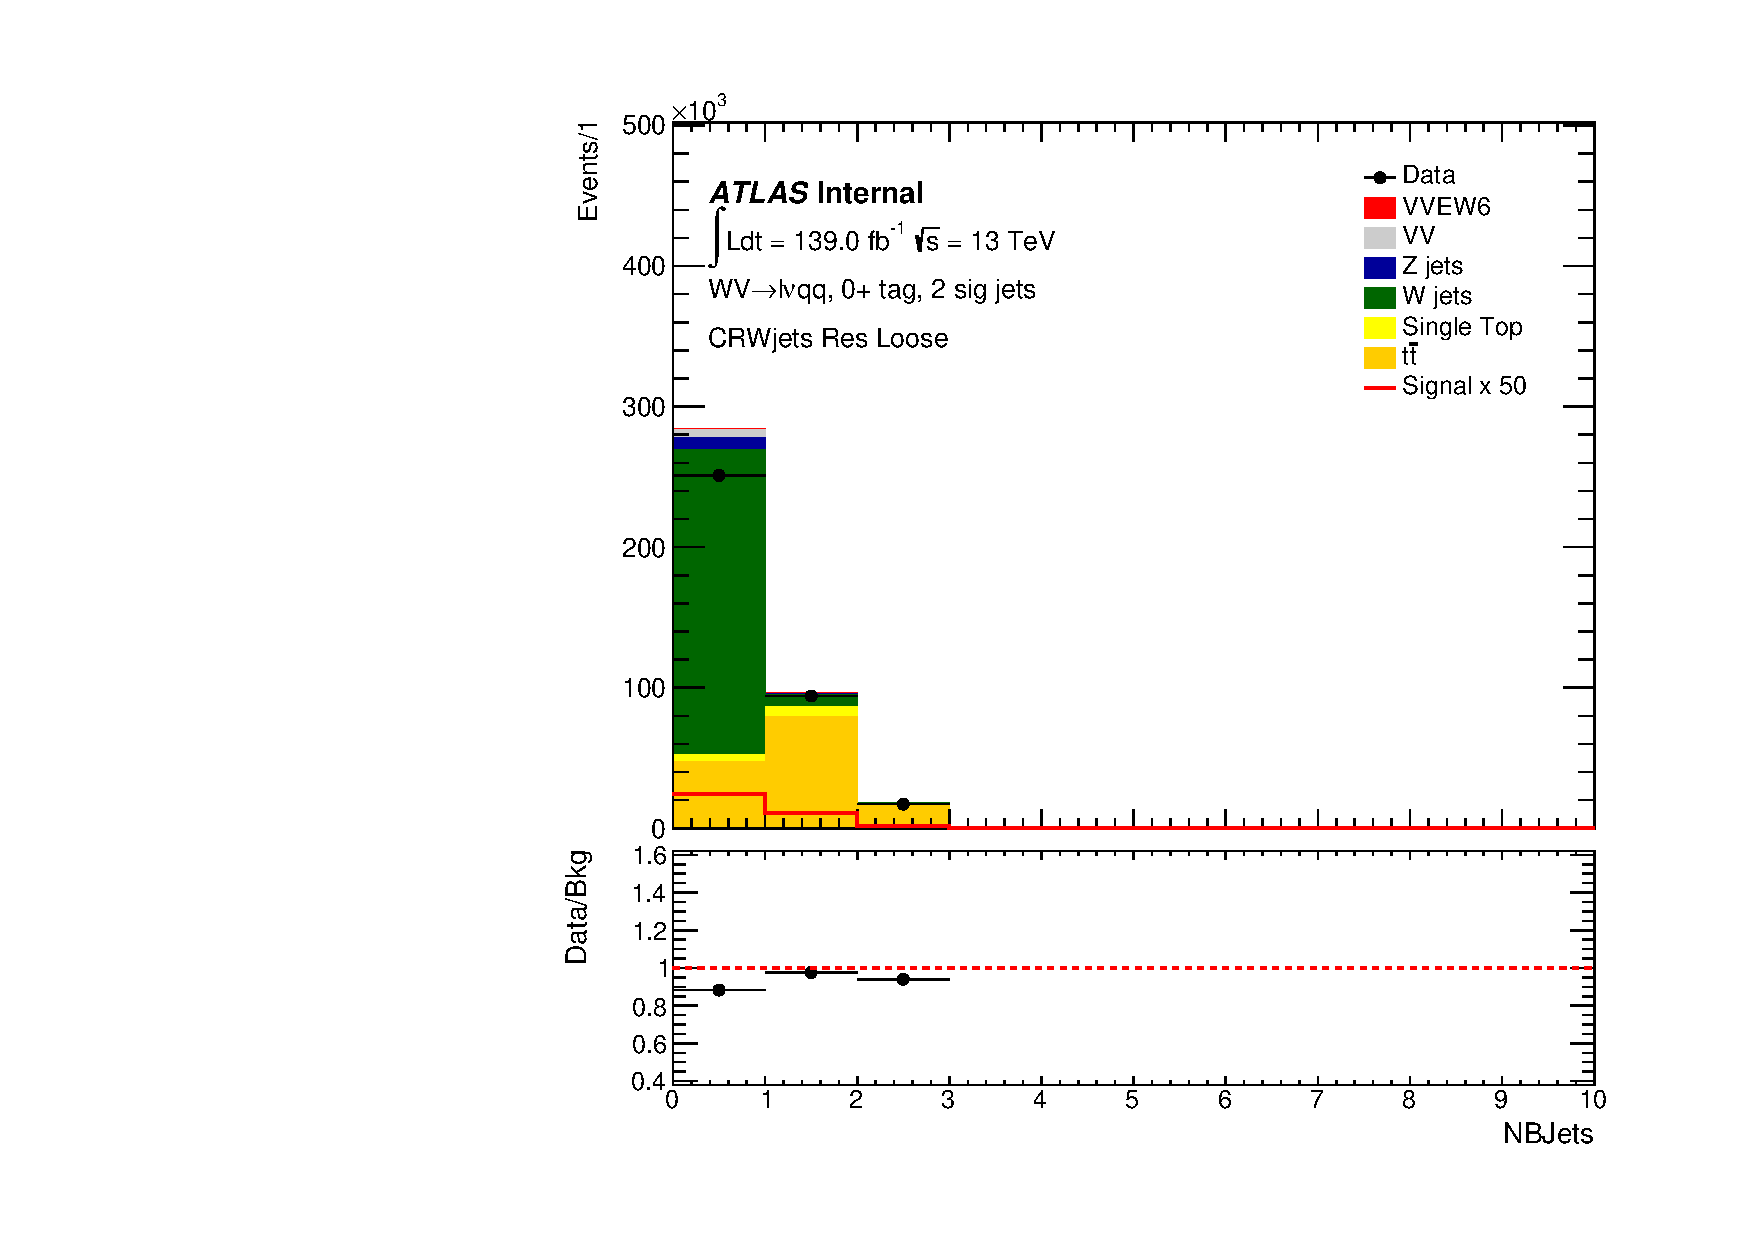
\includegraphics[width=0.3\textwidth]{figures/CRPlots/CRWjets_Res_Loose/stacked_plot_NBJets.pdf}}
    \subfloat[]{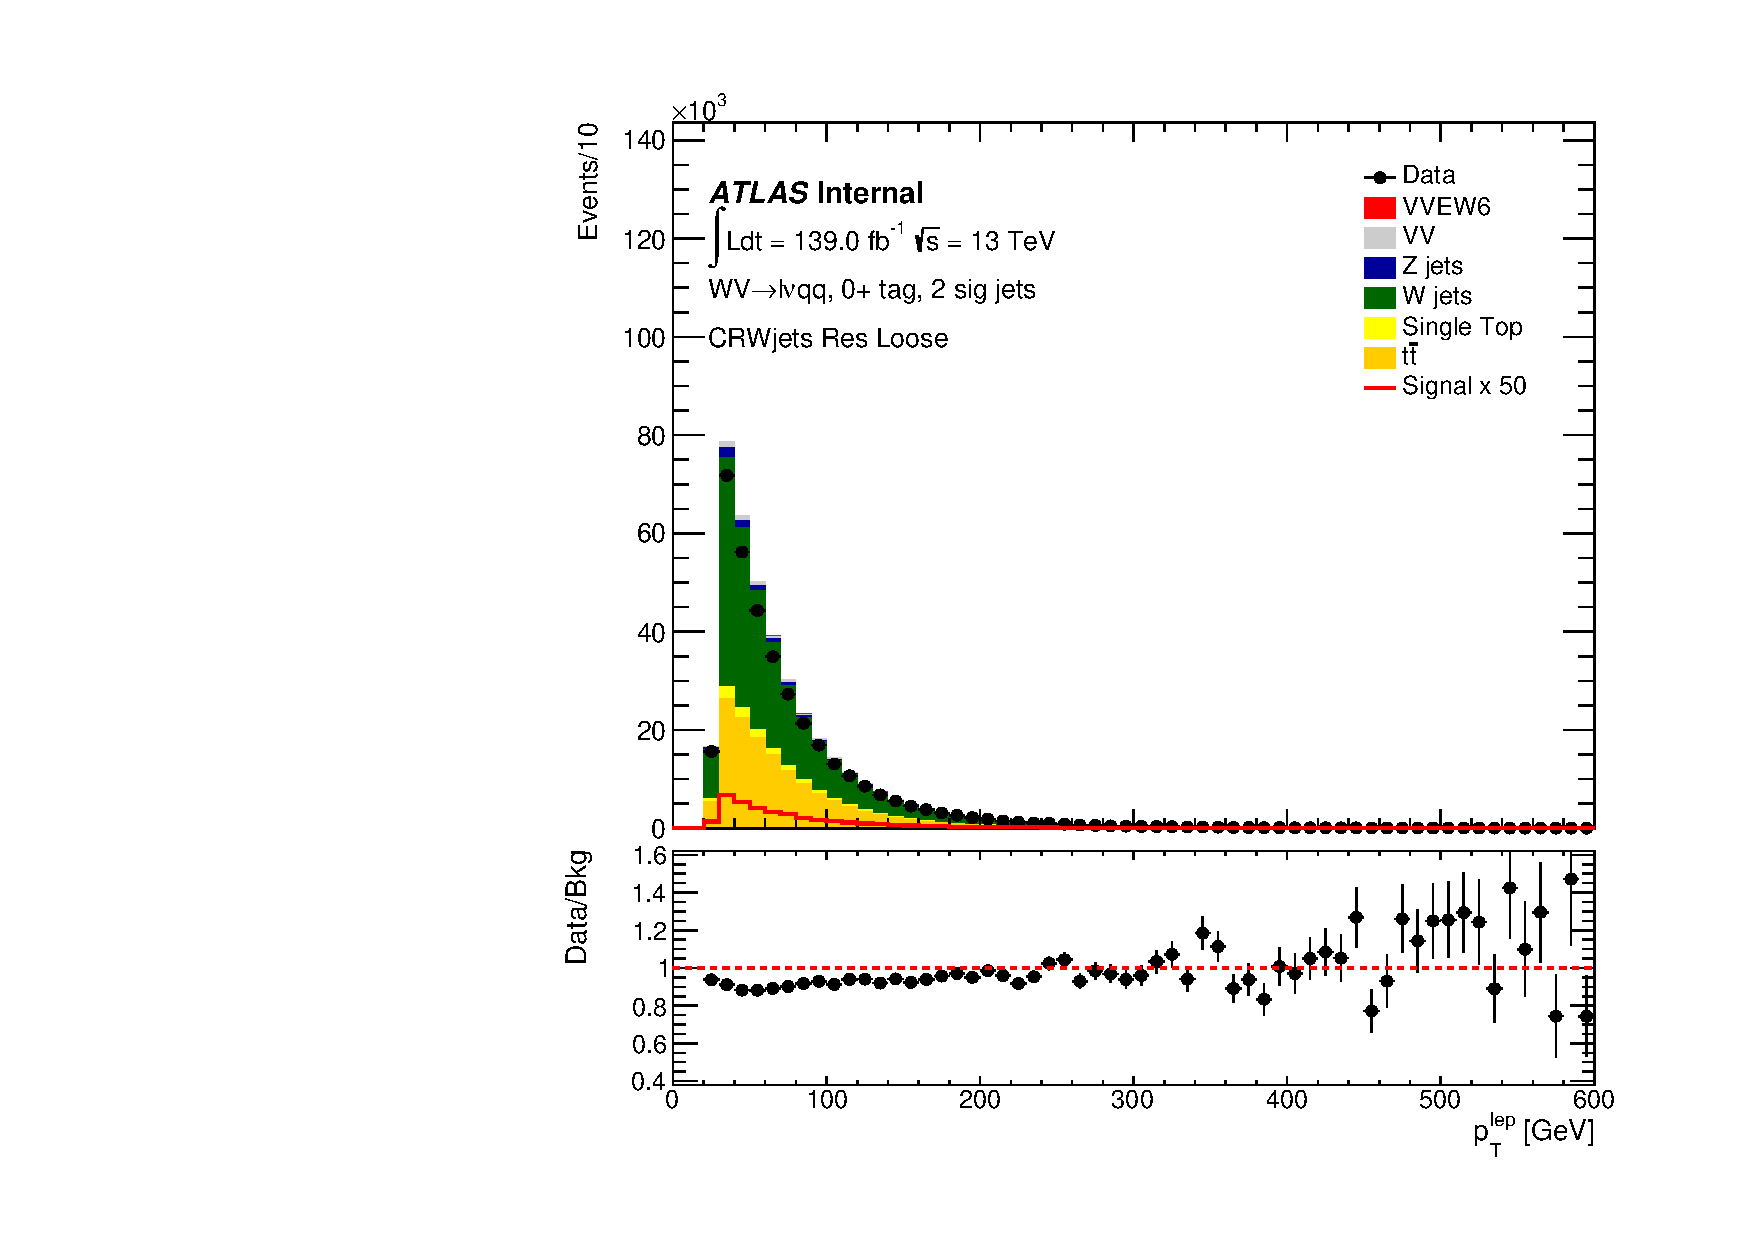
\includegraphics[width=0.3\textwidth]{figures/CRPlots/CRWjets_Res_Loose/stacked_plot_lep_pt.pdf}}  %%\\
    \caption{Data-MC checks for the resolved loose \Wjets control region in the \olep channel.}
    \label{fig:CRWjetResLoosePlots1Lep}
\end{figure}


\begin{figure}[ht]
    \centering
    \subfloat[]{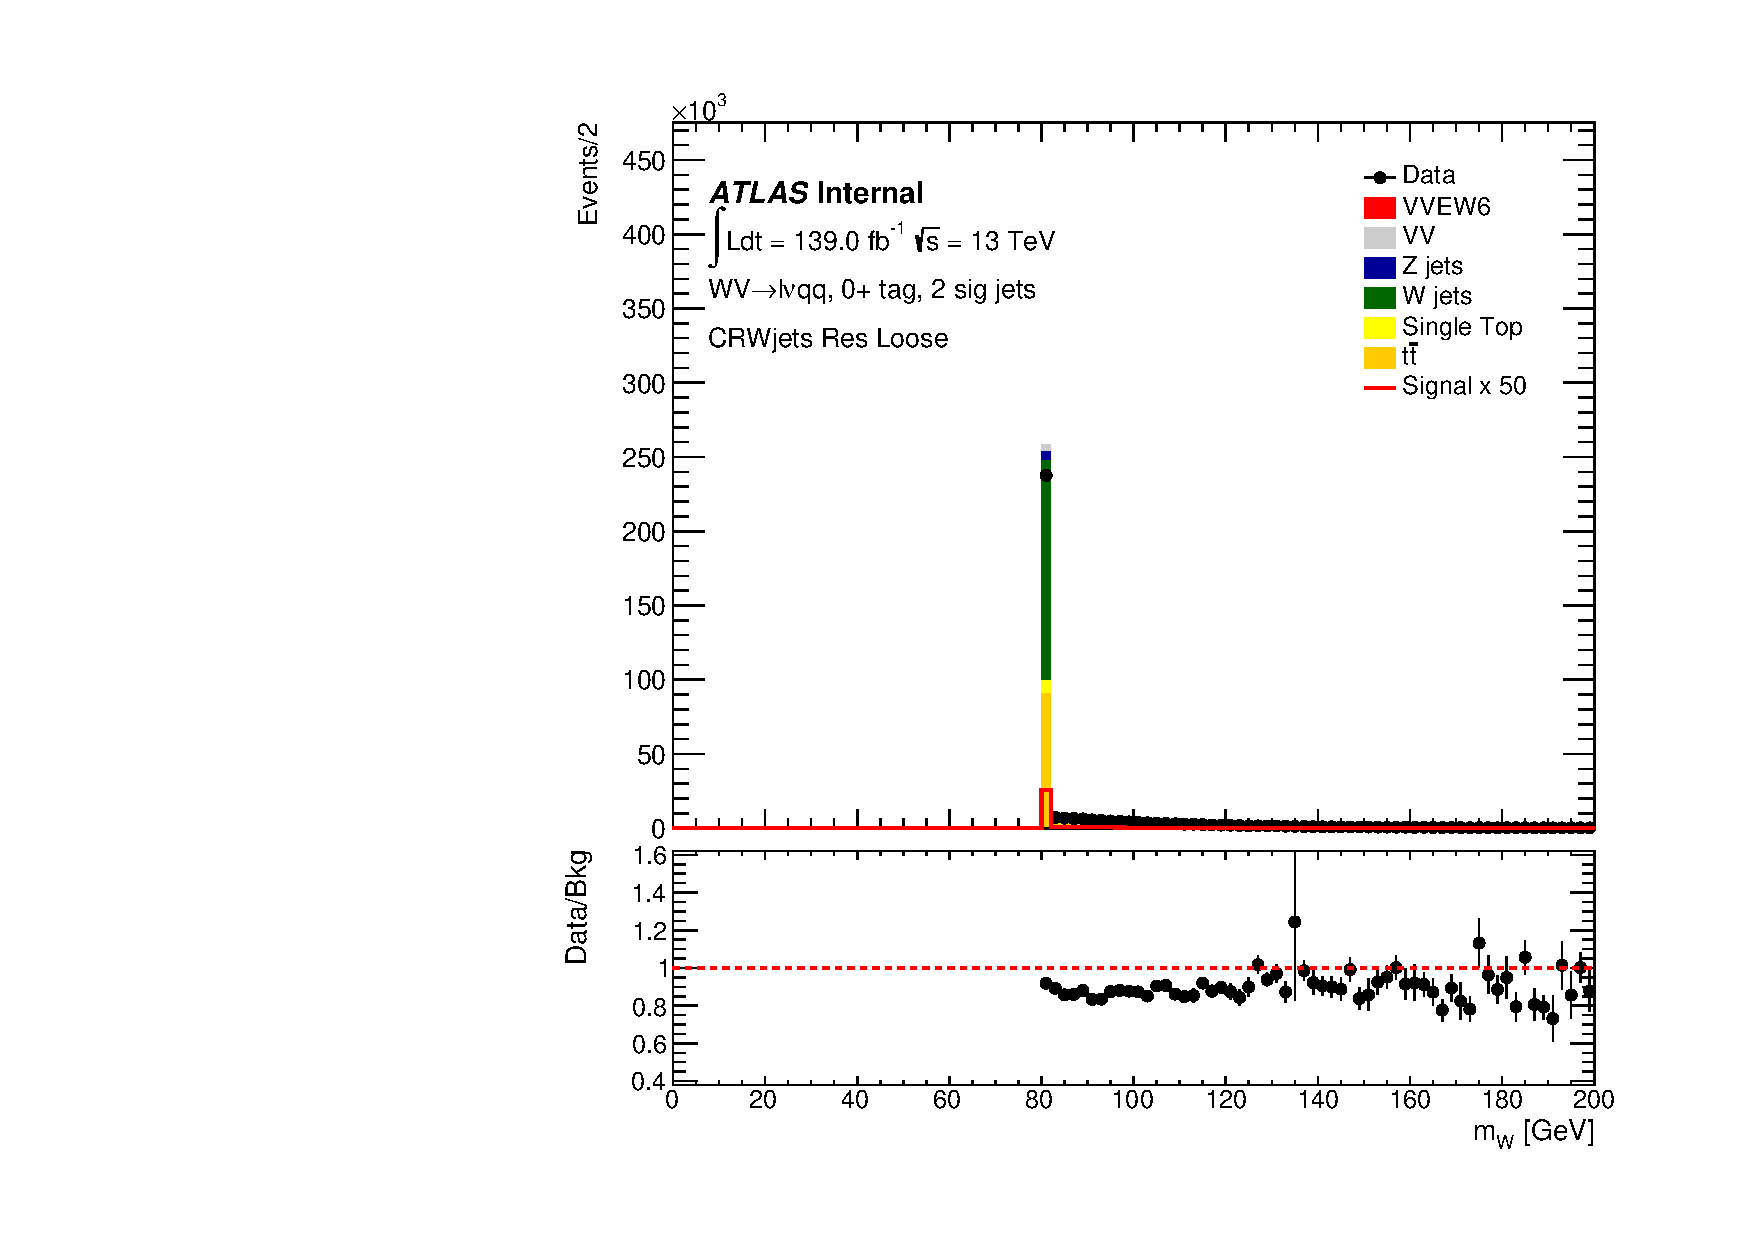
\includegraphics[width=0.3\textwidth]{figures/CRPlots/CRWjets_Res_Loose/stacked_plot_W_m.pdf}}
    \subfloat[]{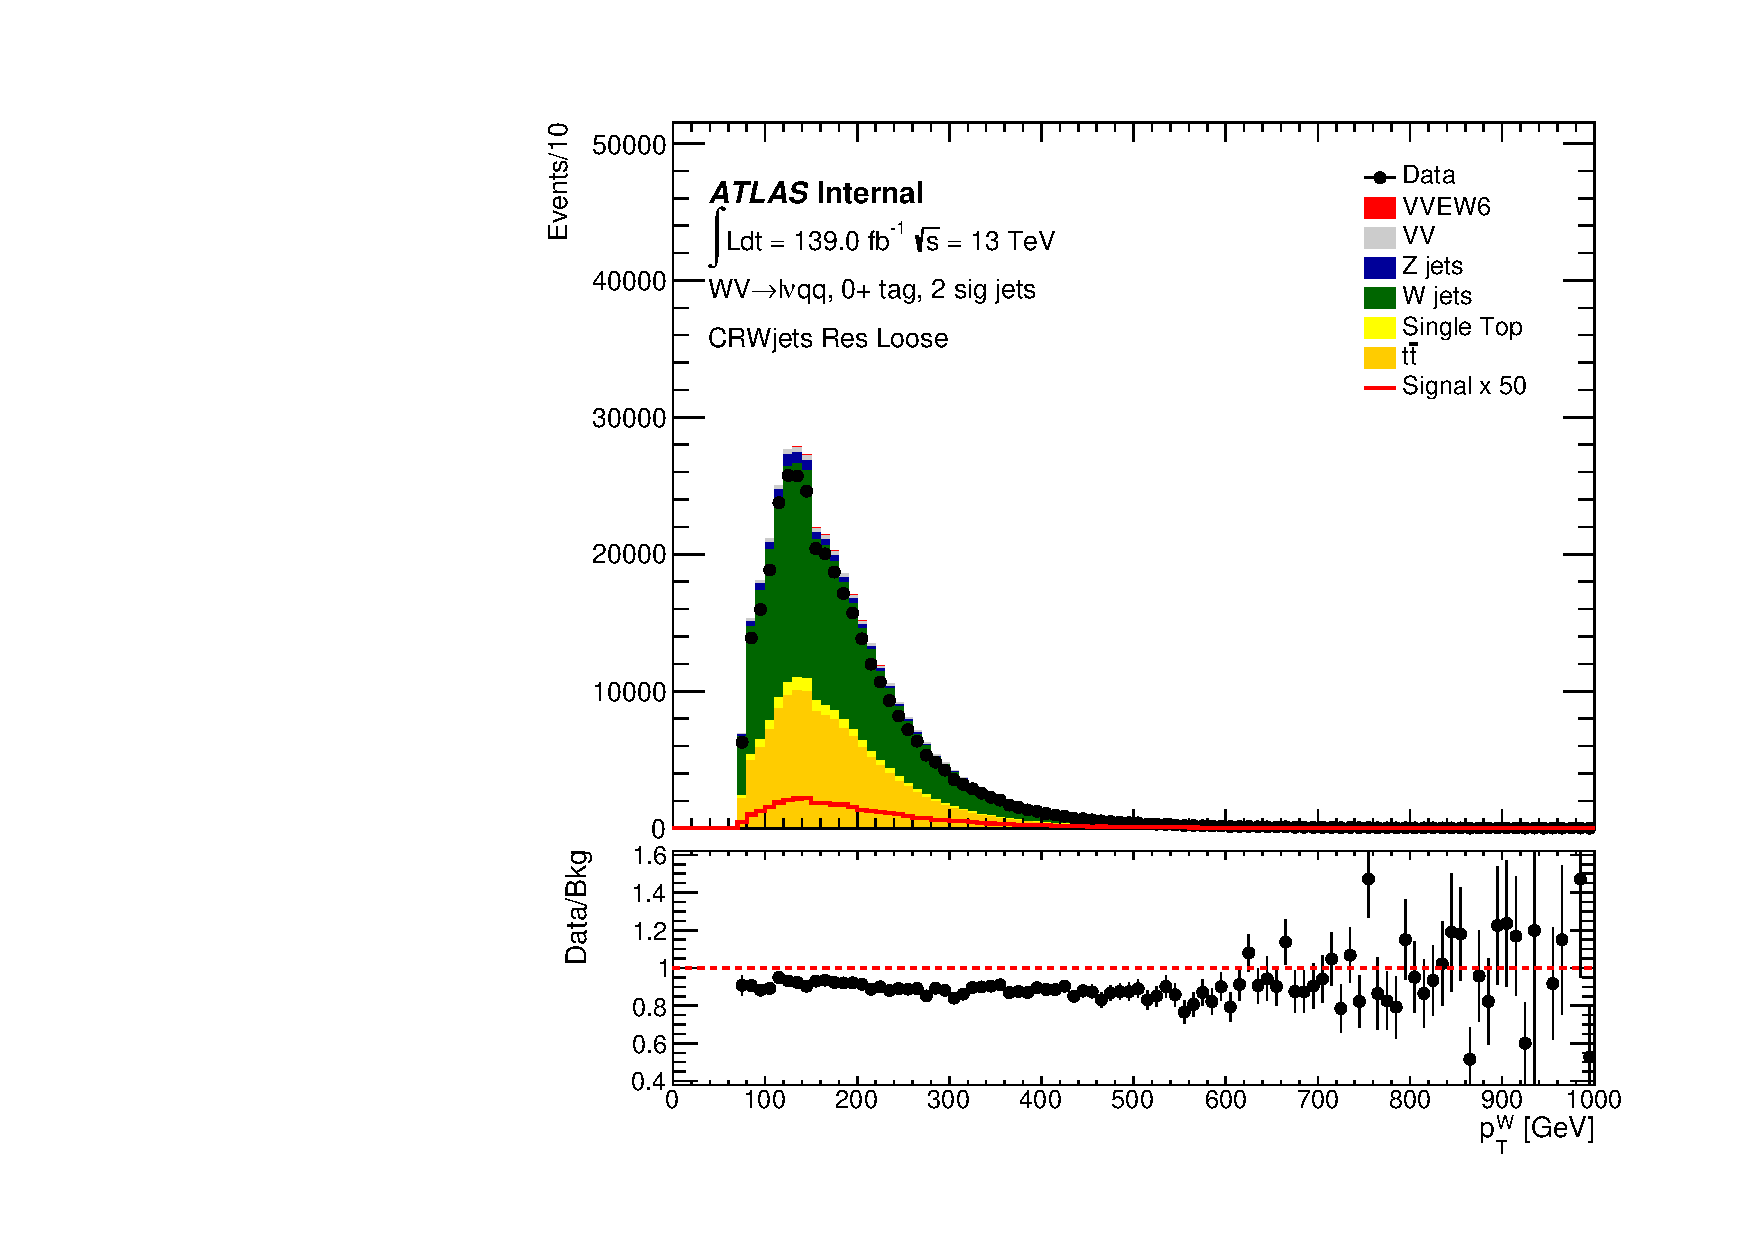
\includegraphics[width=0.3\textwidth]{figures/CRPlots/CRWjets_Res_Loose/stacked_plot_W_pt.pdf}}
    \subfloat[]{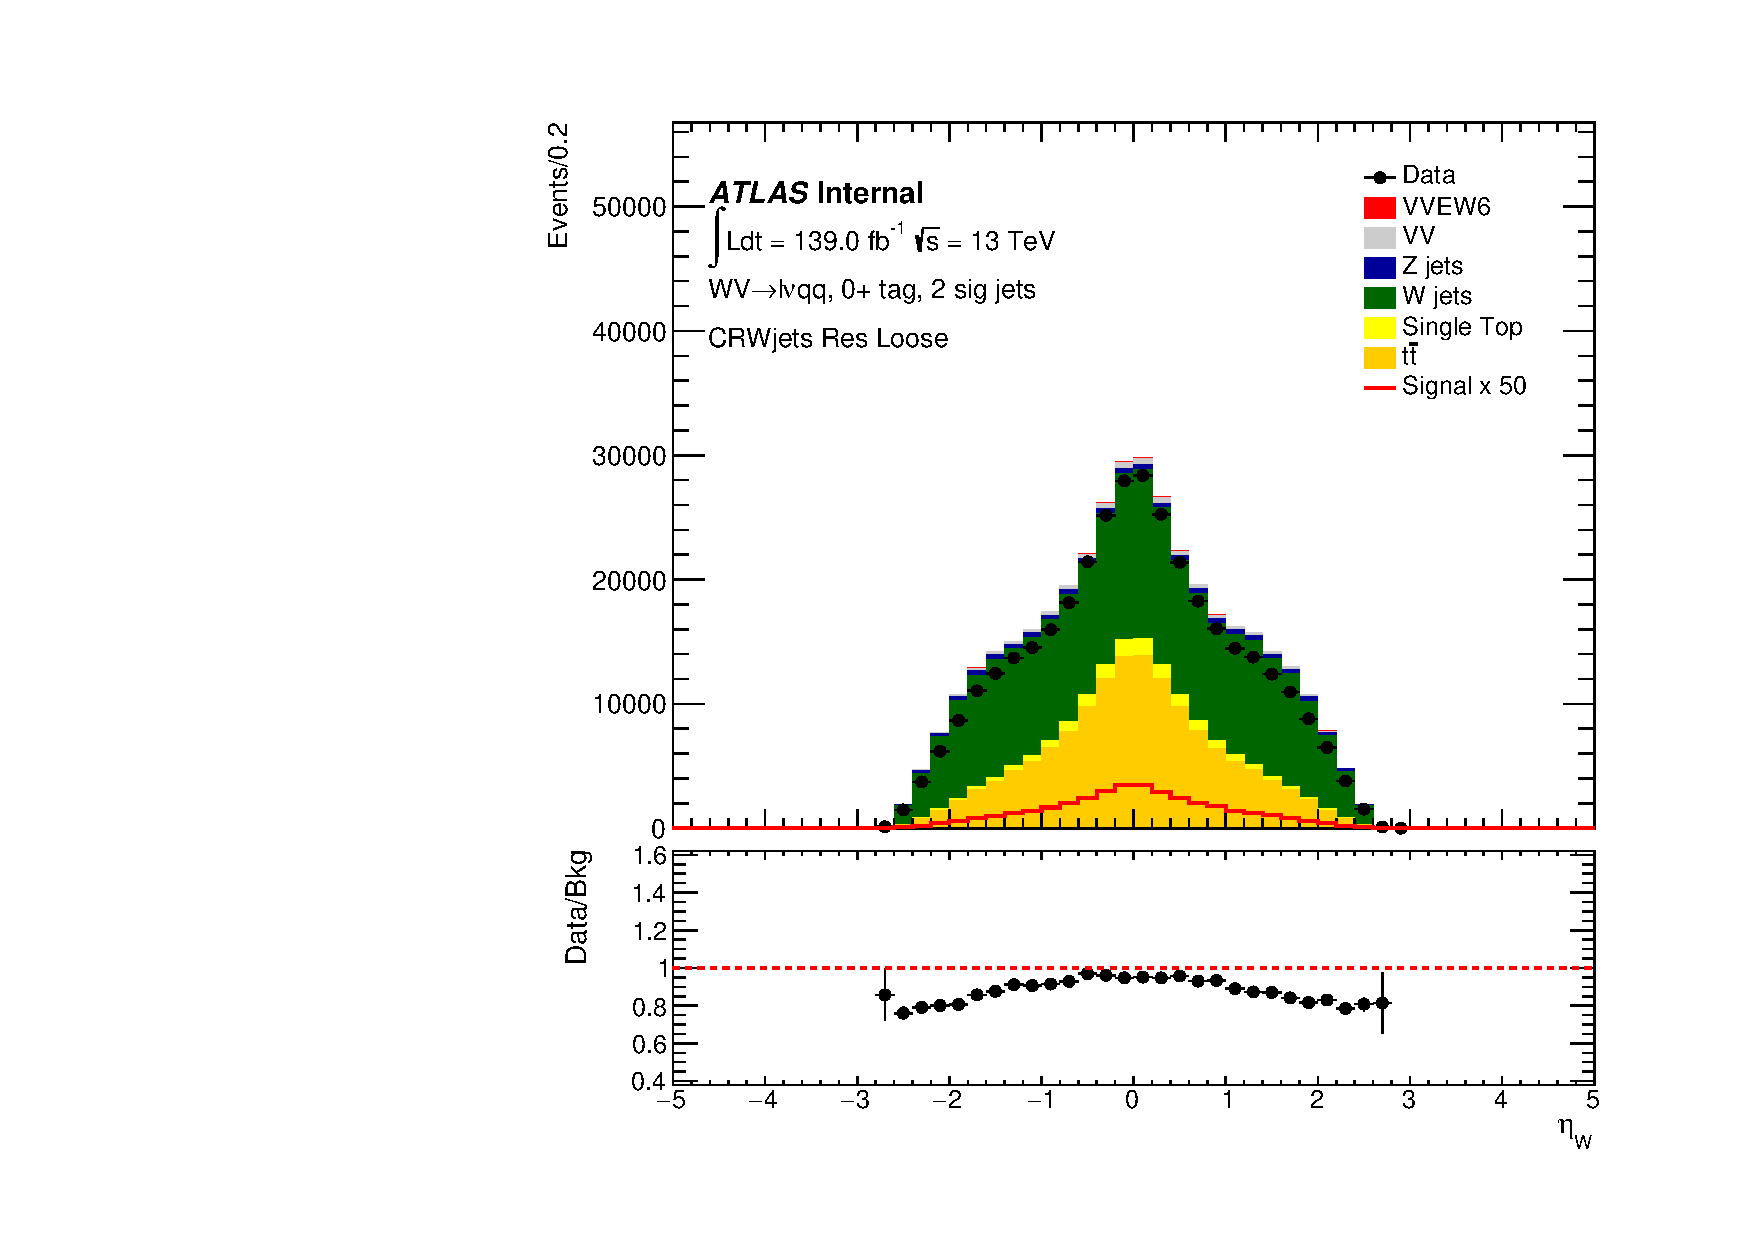
\includegraphics[width=0.3\textwidth]{figures/CRPlots/CRWjets_Res_Loose/stacked_plot_W_eta.pdf}} \\
    \subfloat[]{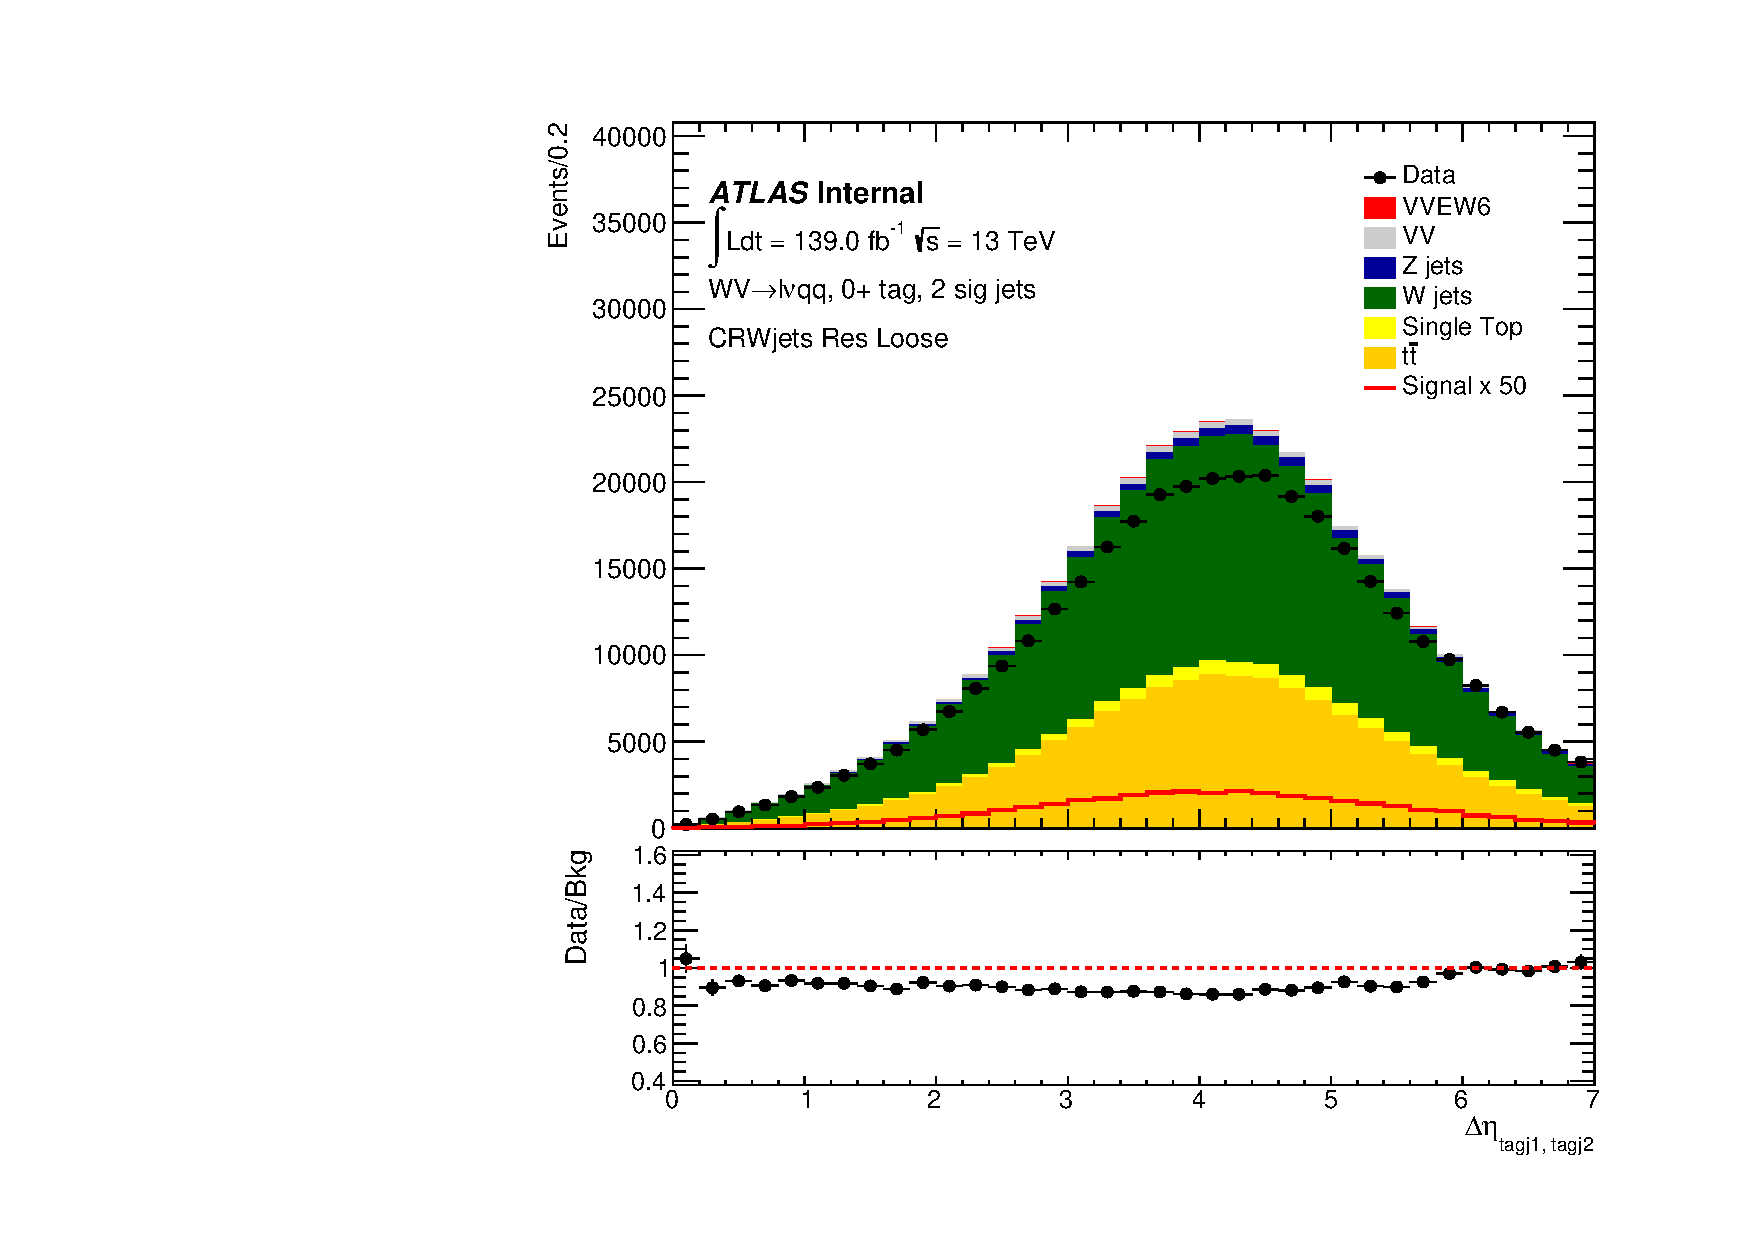
\includegraphics[width=0.3\textwidth]{figures/CRPlots/CRWjets_Res_Loose/stacked_plot_resolved_tagJdEta.pdf}}
    \subfloat[]{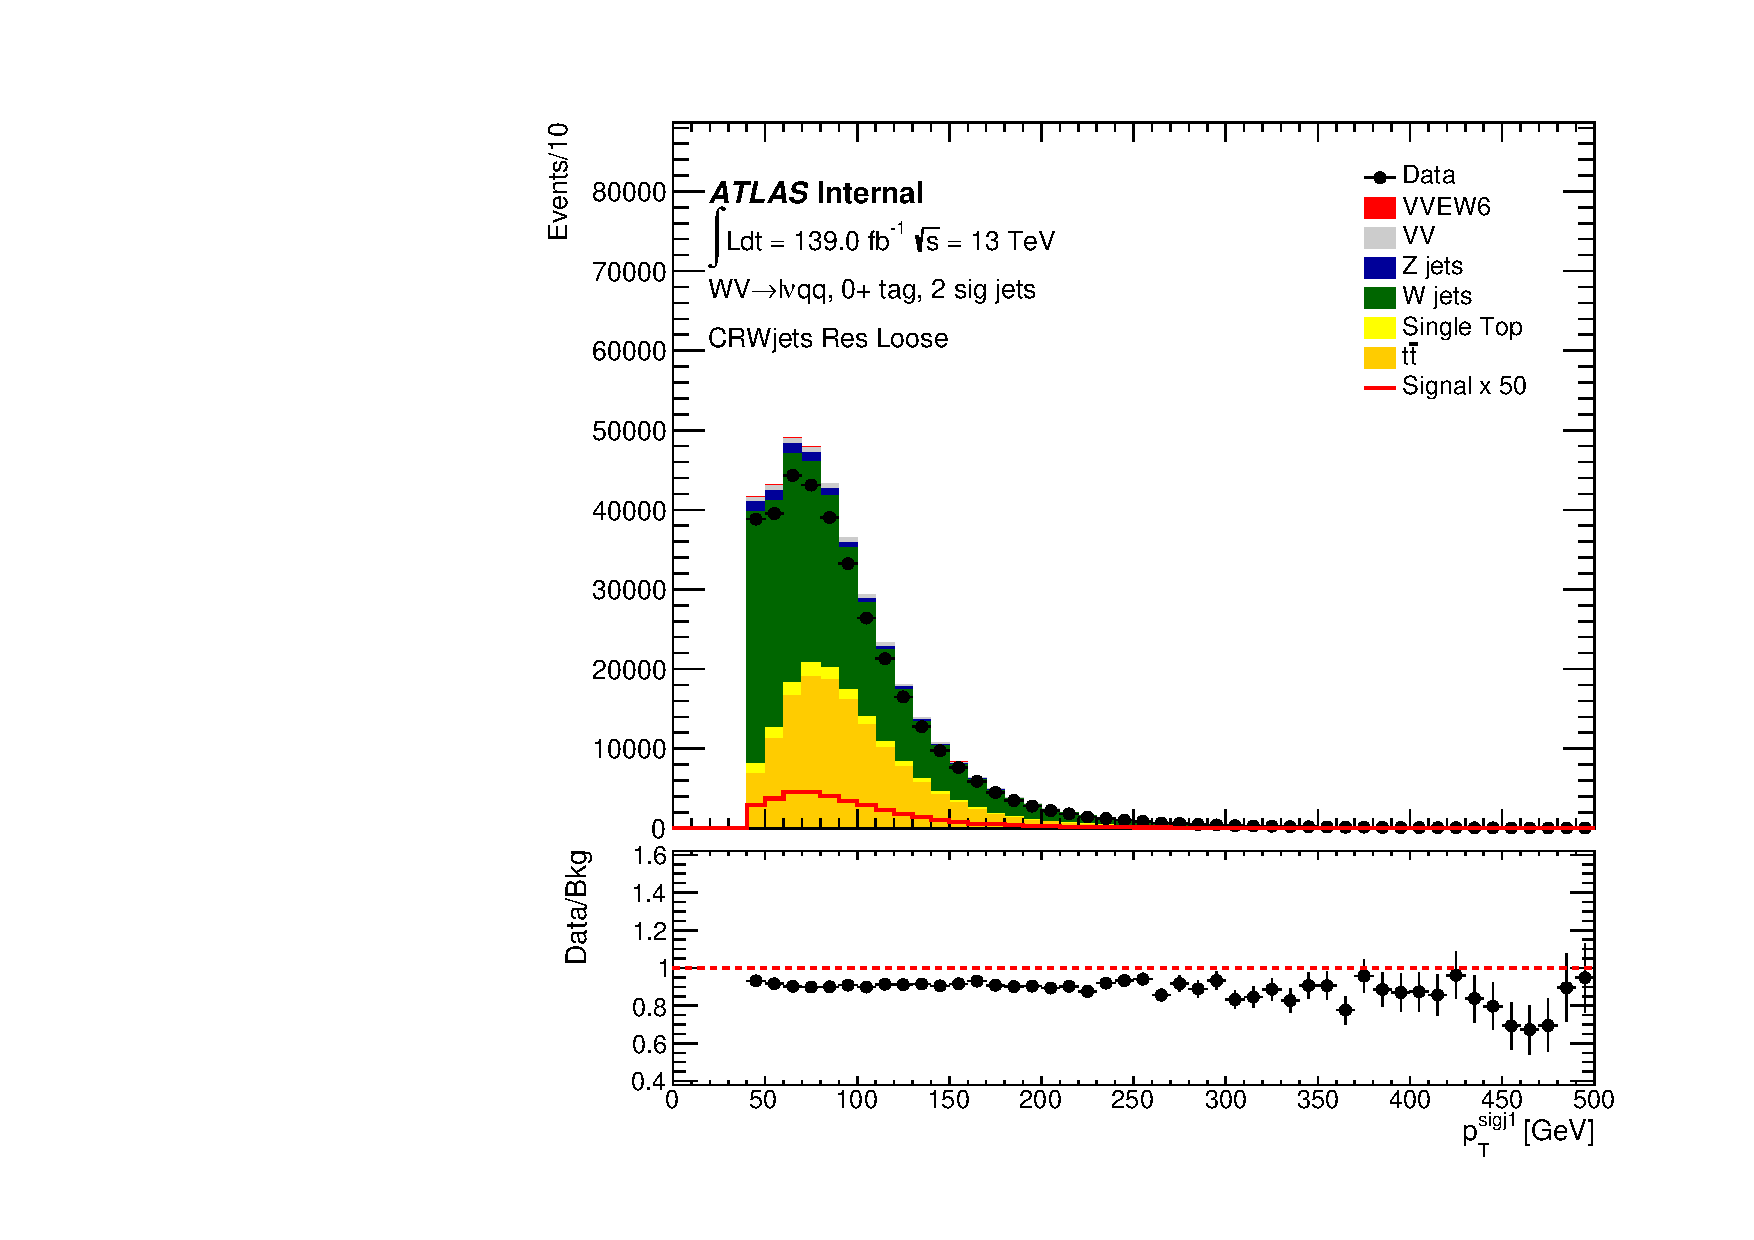
\includegraphics[width=0.3\textwidth]{figures/CRPlots/CRWjets_Res_Loose/stacked_plot_sigJ1_pt.pdf}}
    \subfloat[]{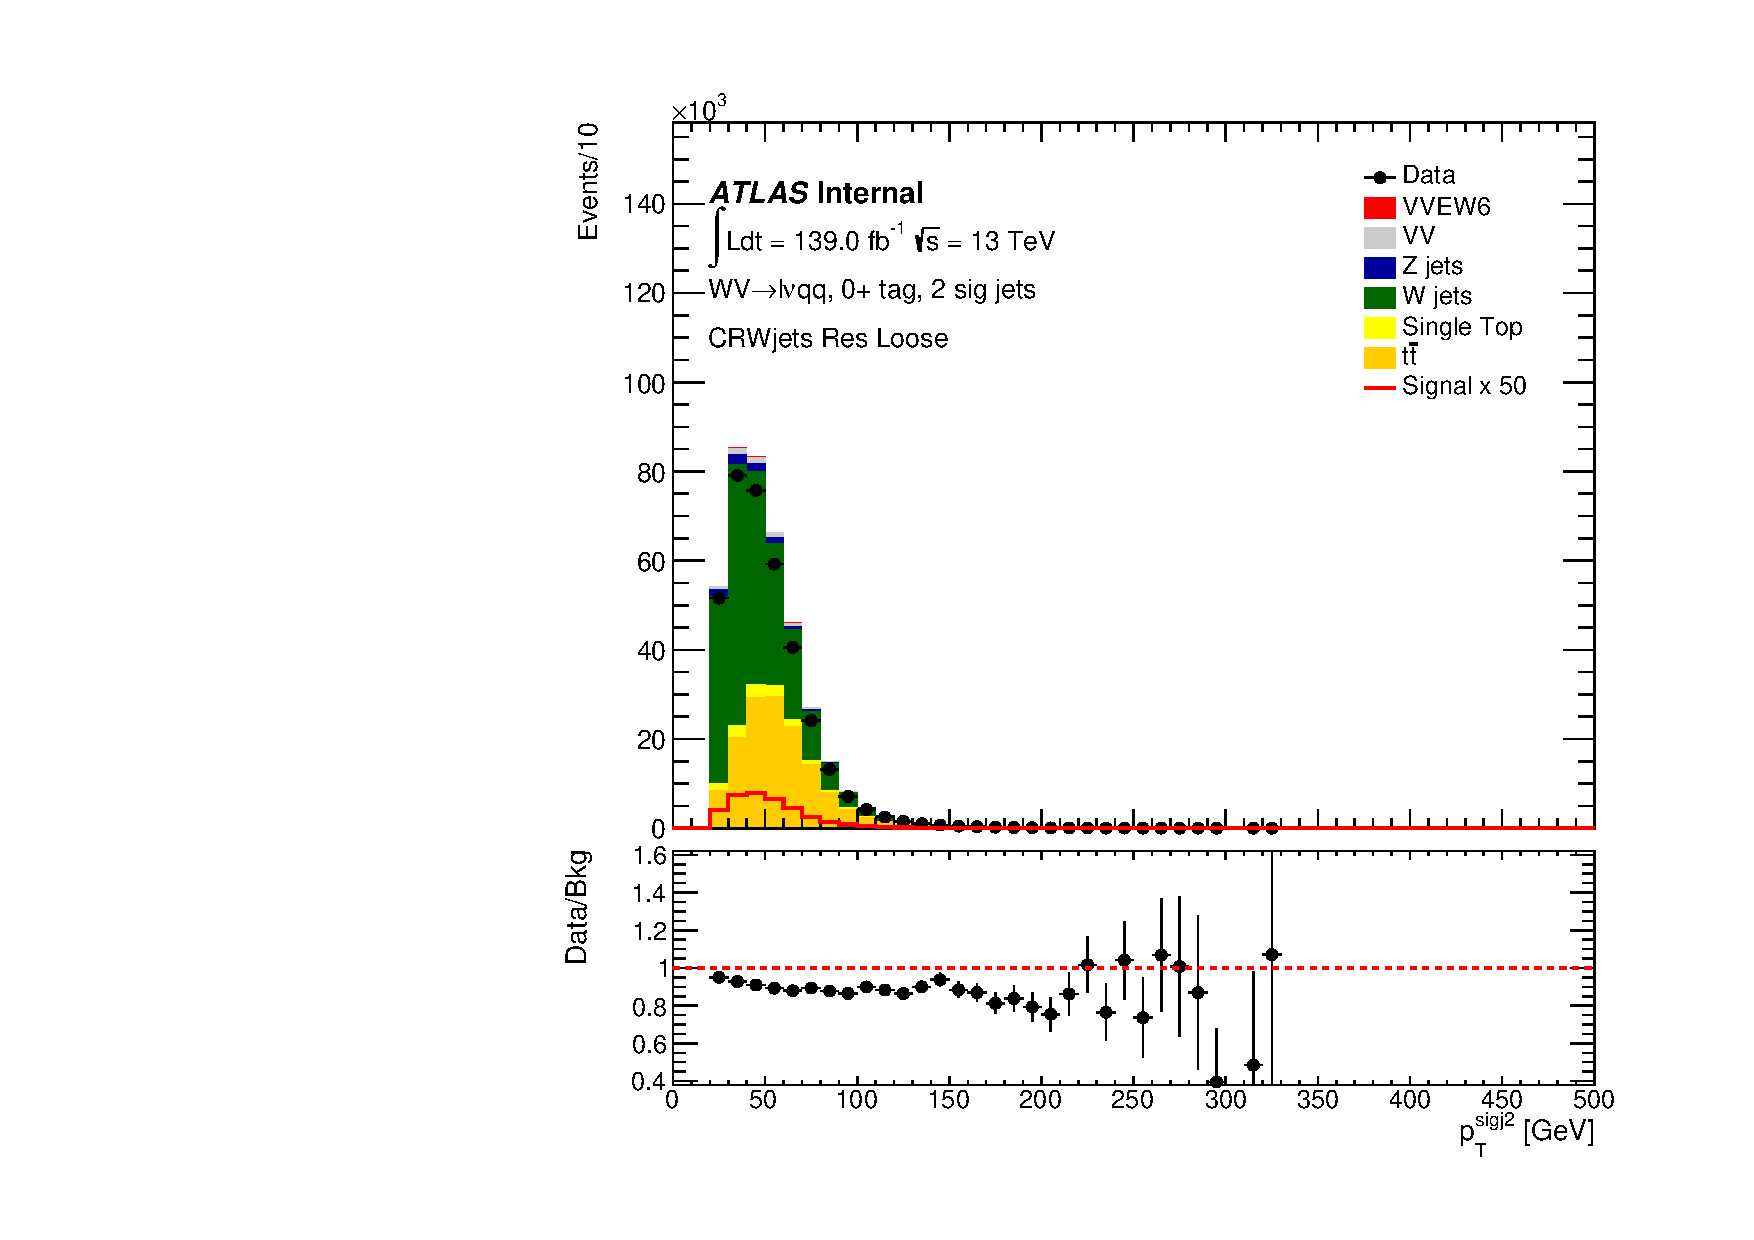
\includegraphics[width=0.3\textwidth]{figures/CRPlots/CRWjets_Res_Loose/stacked_plot_sigJ2_pt.pdf}} \\
    \subfloat[]{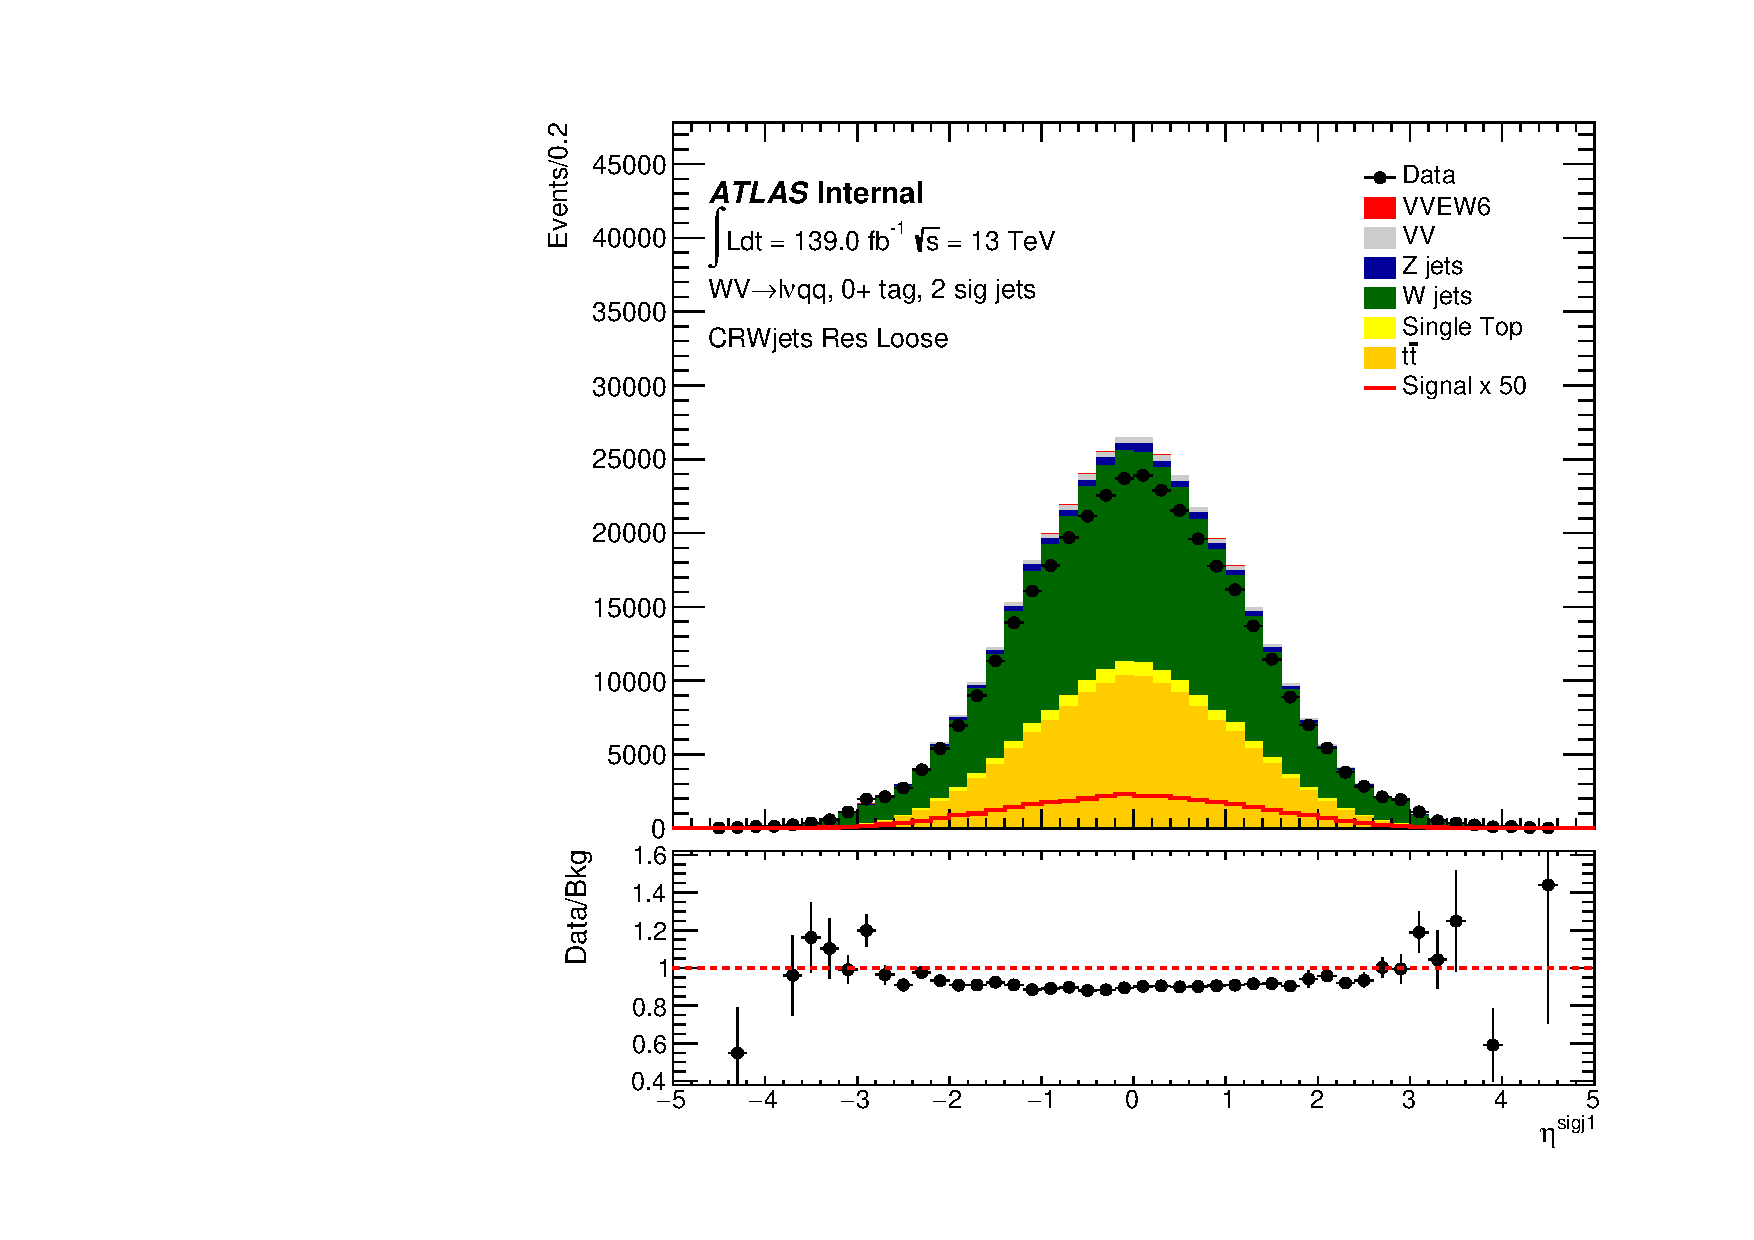
\includegraphics[width=0.3\textwidth]{figures/CRPlots/CRWjets_Res_Loose/stacked_plot_sigJ1_eta.pdf}}
    \subfloat[]{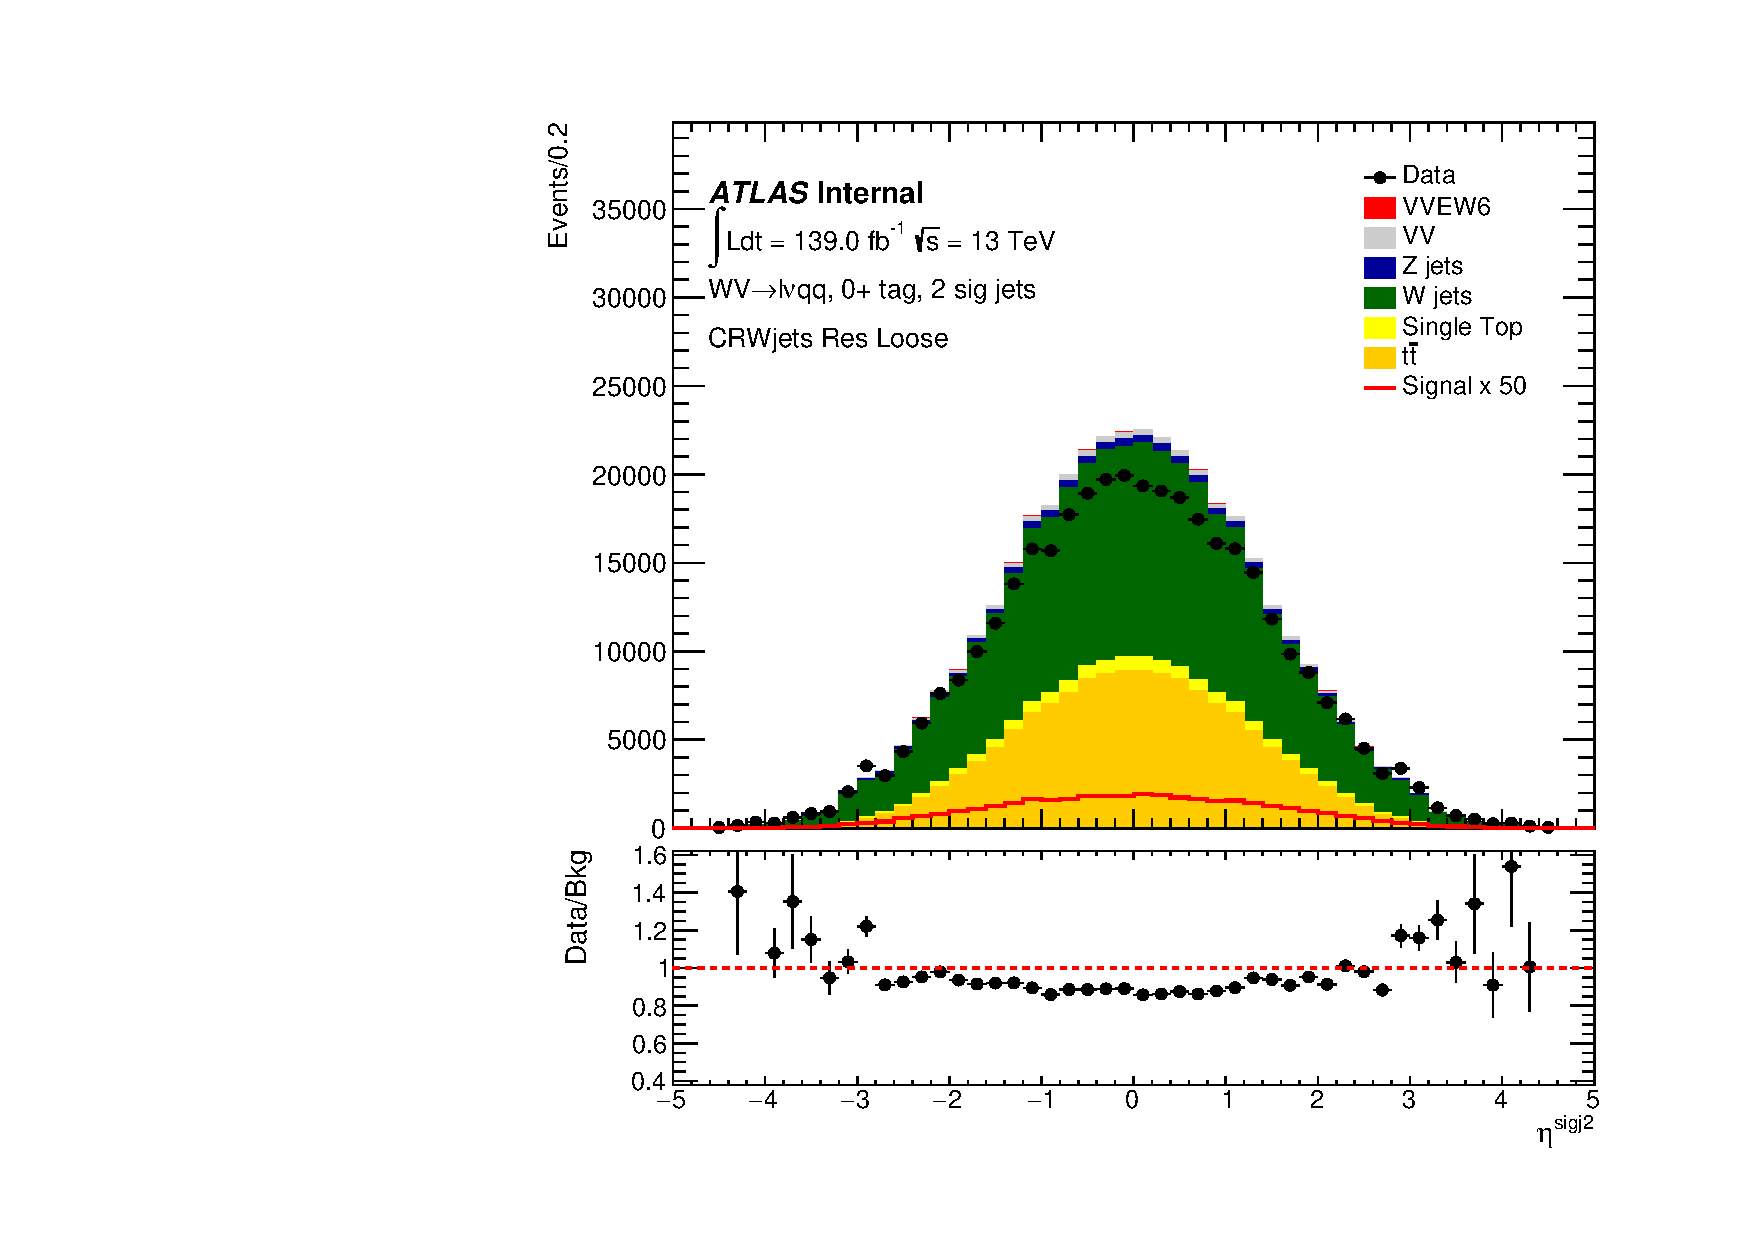
\includegraphics[width=0.3\textwidth]{figures/CRPlots/CRWjets_Res_Loose/stacked_plot_sigJ2_eta.pdf}} \\
    \subfloat[]{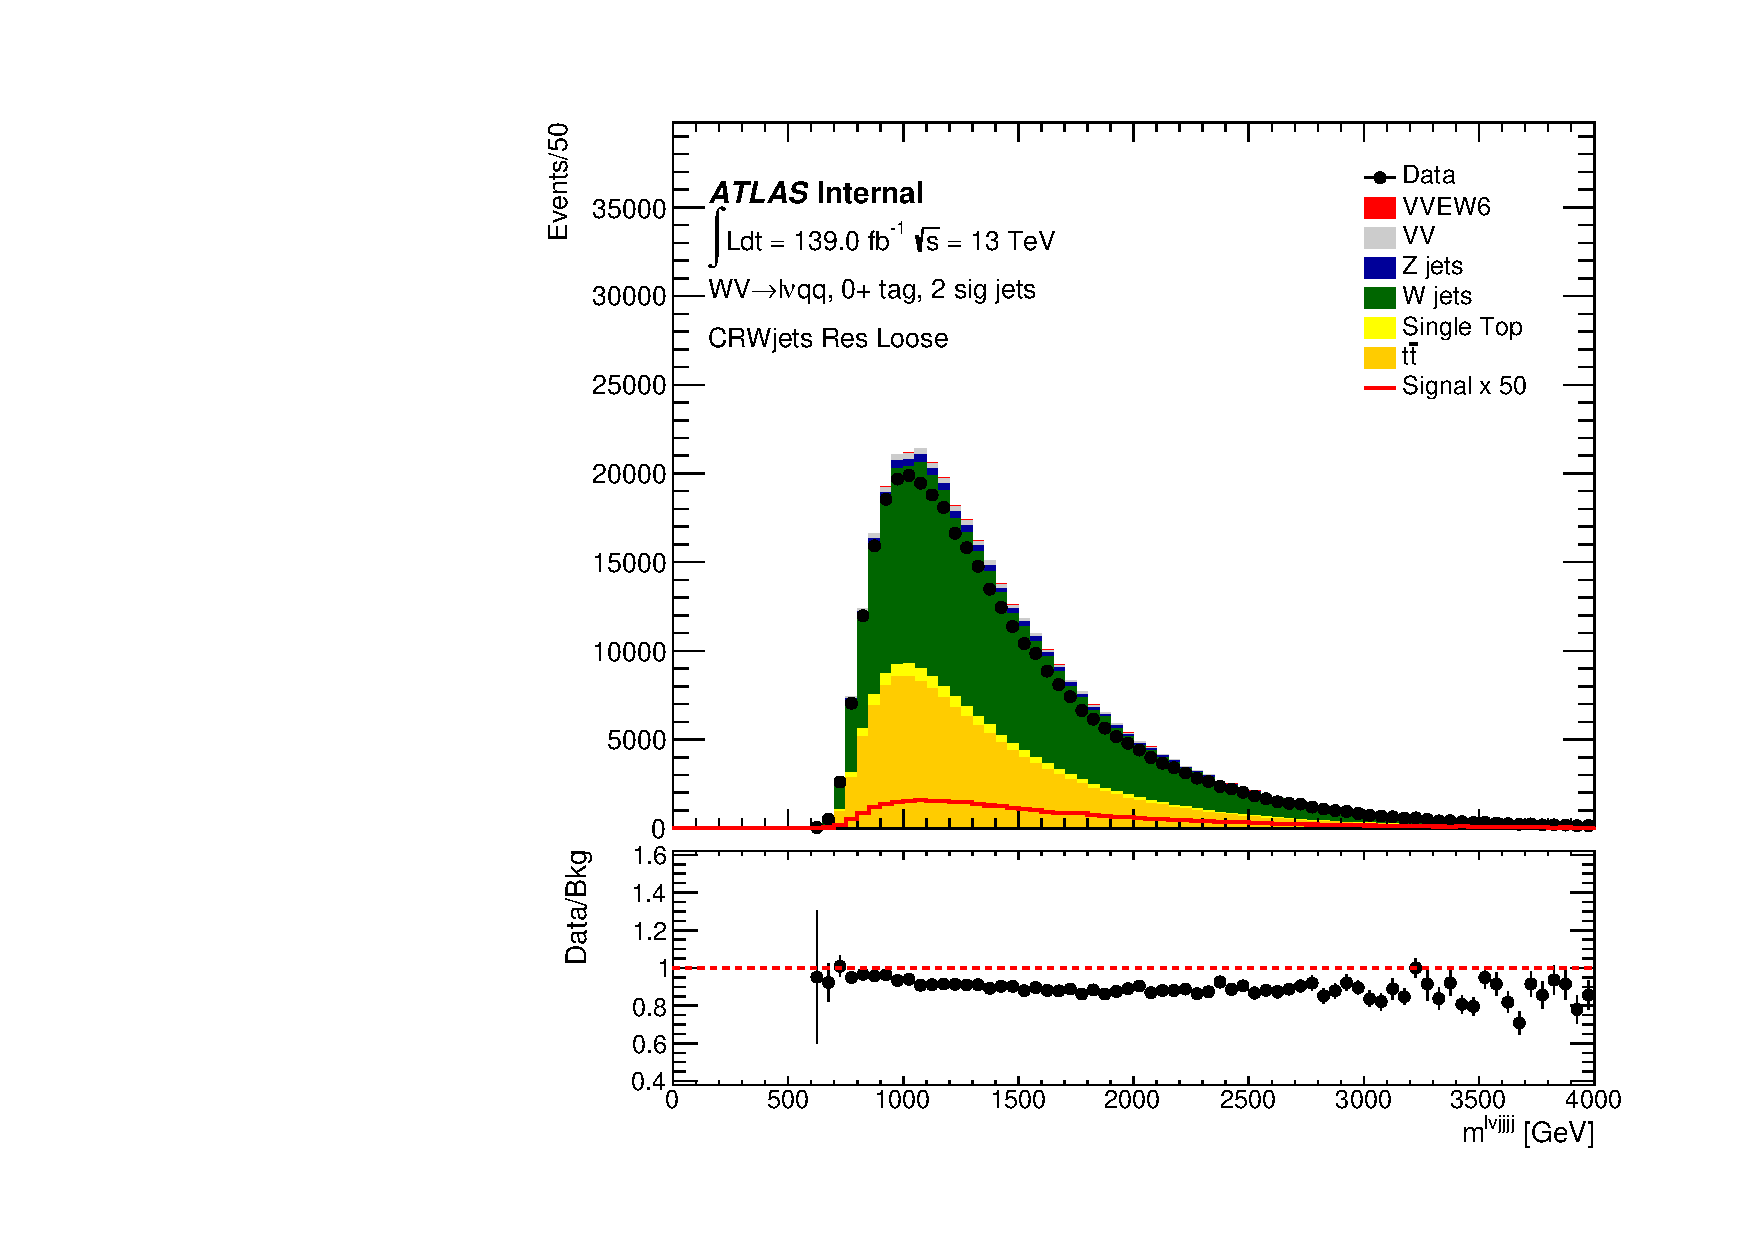
\includegraphics[width=0.3\textwidth]{figures/CRPlots/CRWjets_Res_Loose/stacked_plot_lvjjjjmass.pdf}}
    \subfloat[]{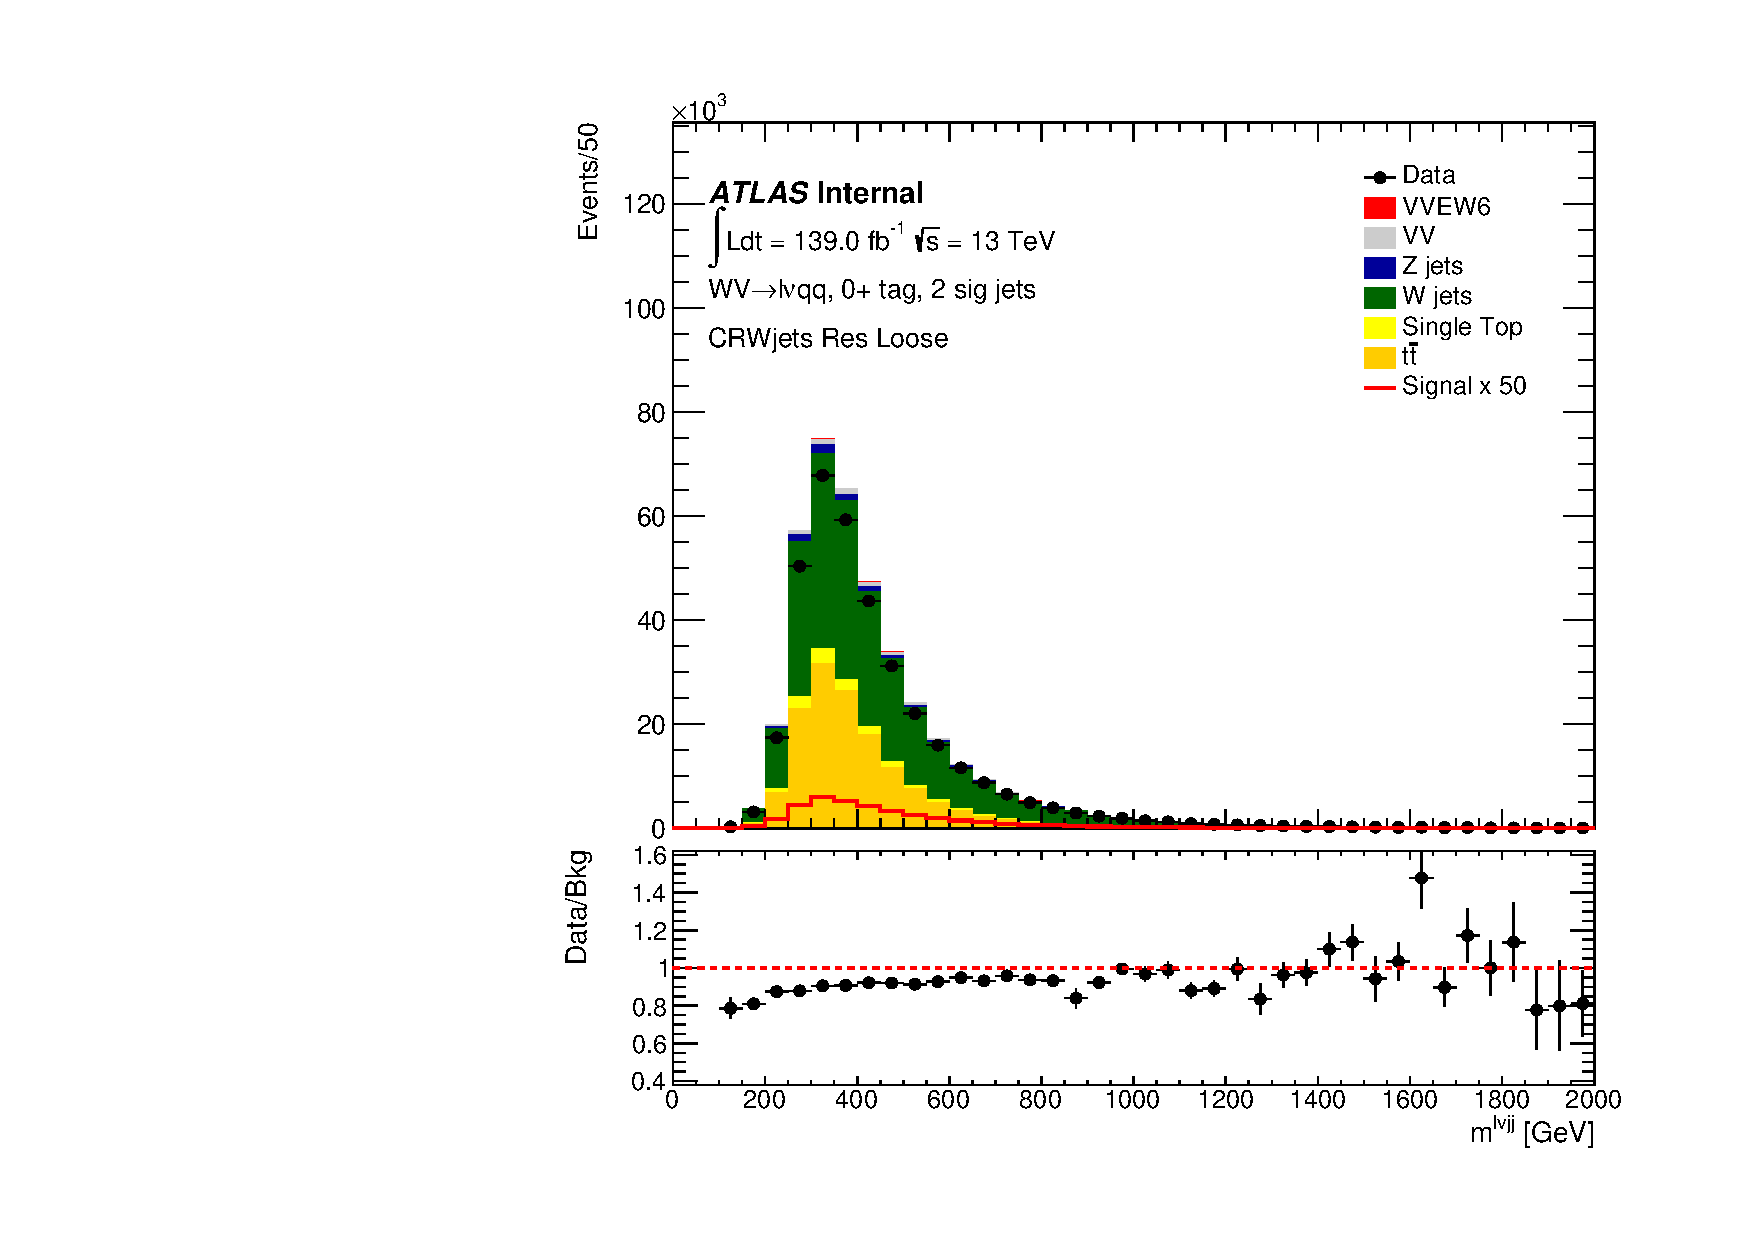
\includegraphics[width=0.3\textwidth]{figures/CRPlots/CRWjets_Res_Loose/stacked_plot_lvjjmass.pdf}}
    \subfloat[]{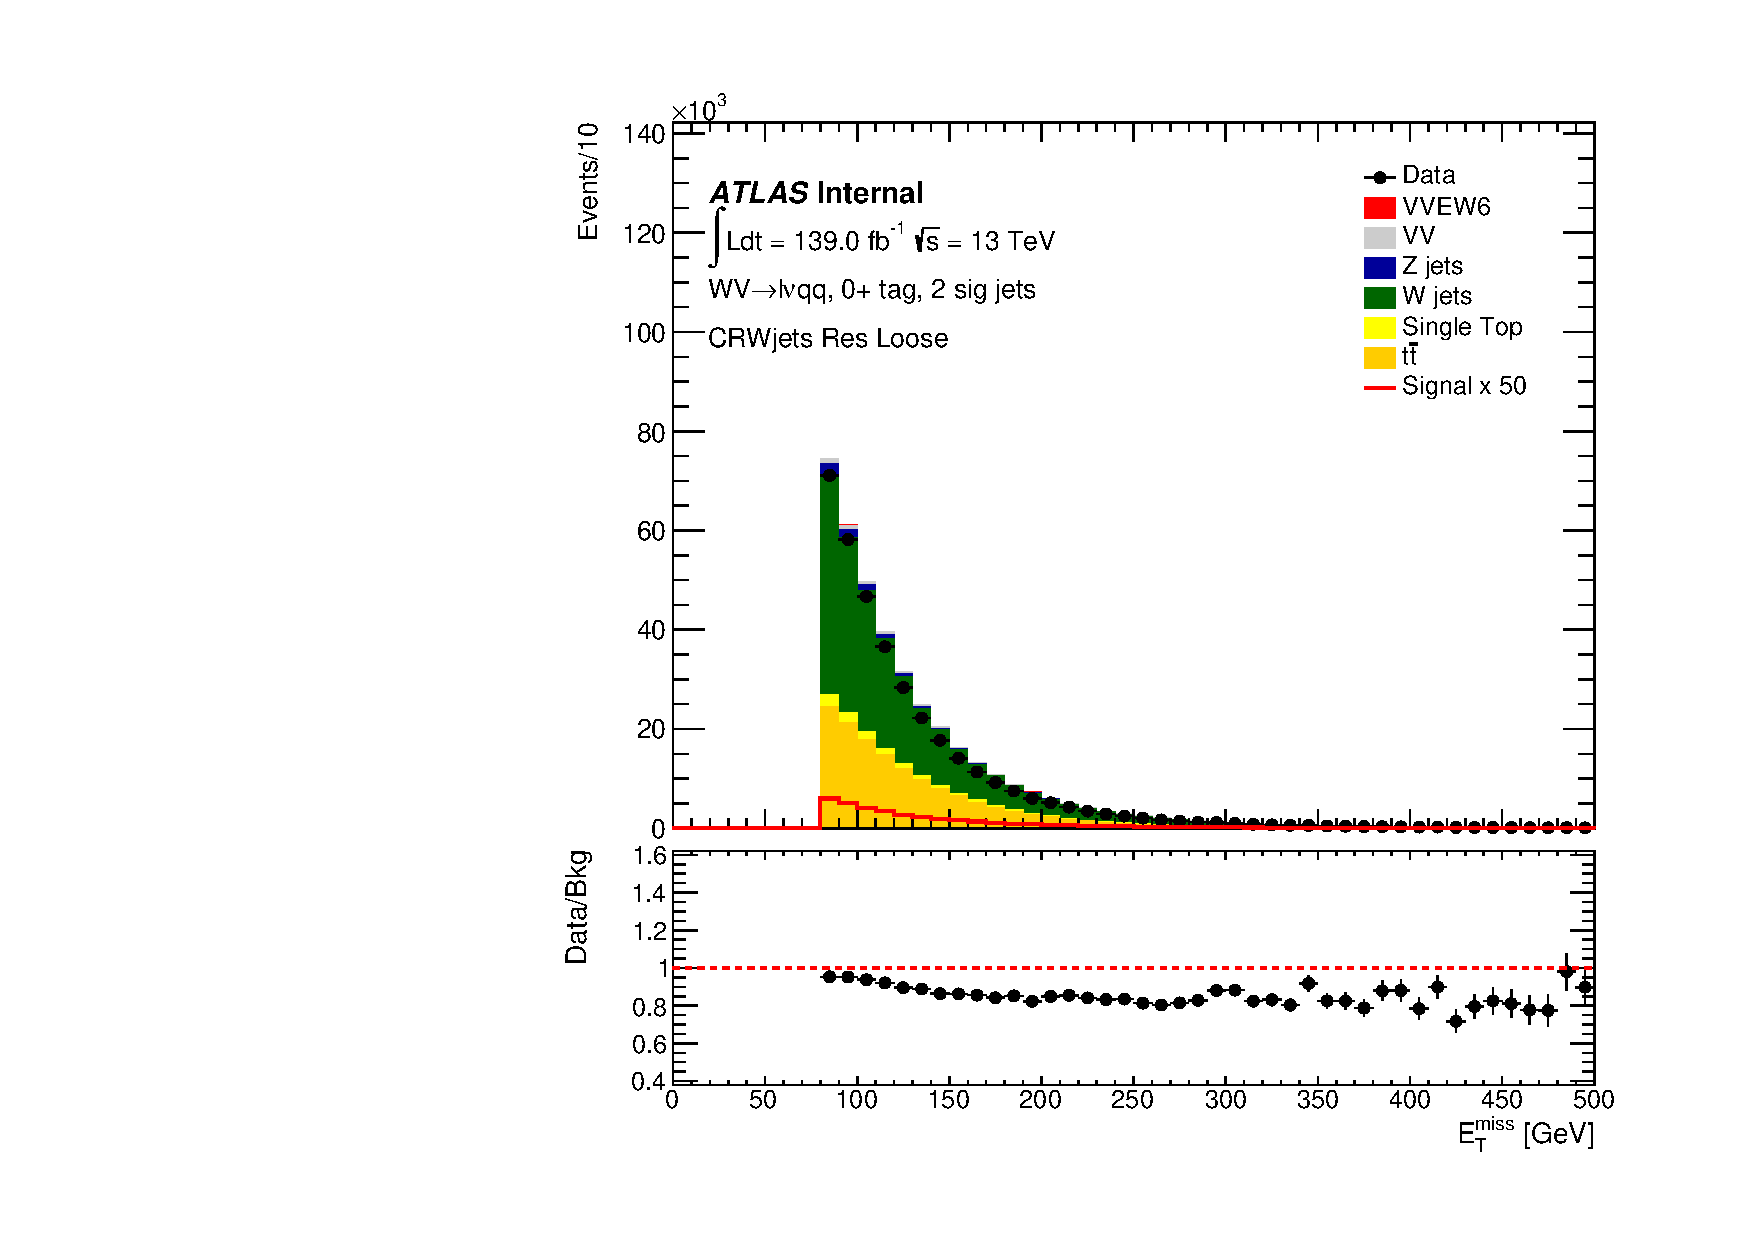
\includegraphics[width=0.3\textwidth]{figures/CRPlots/CRWjets_Res_Loose/stacked_plot_met.pdf}}  %%\\
%%    \subfloat[]{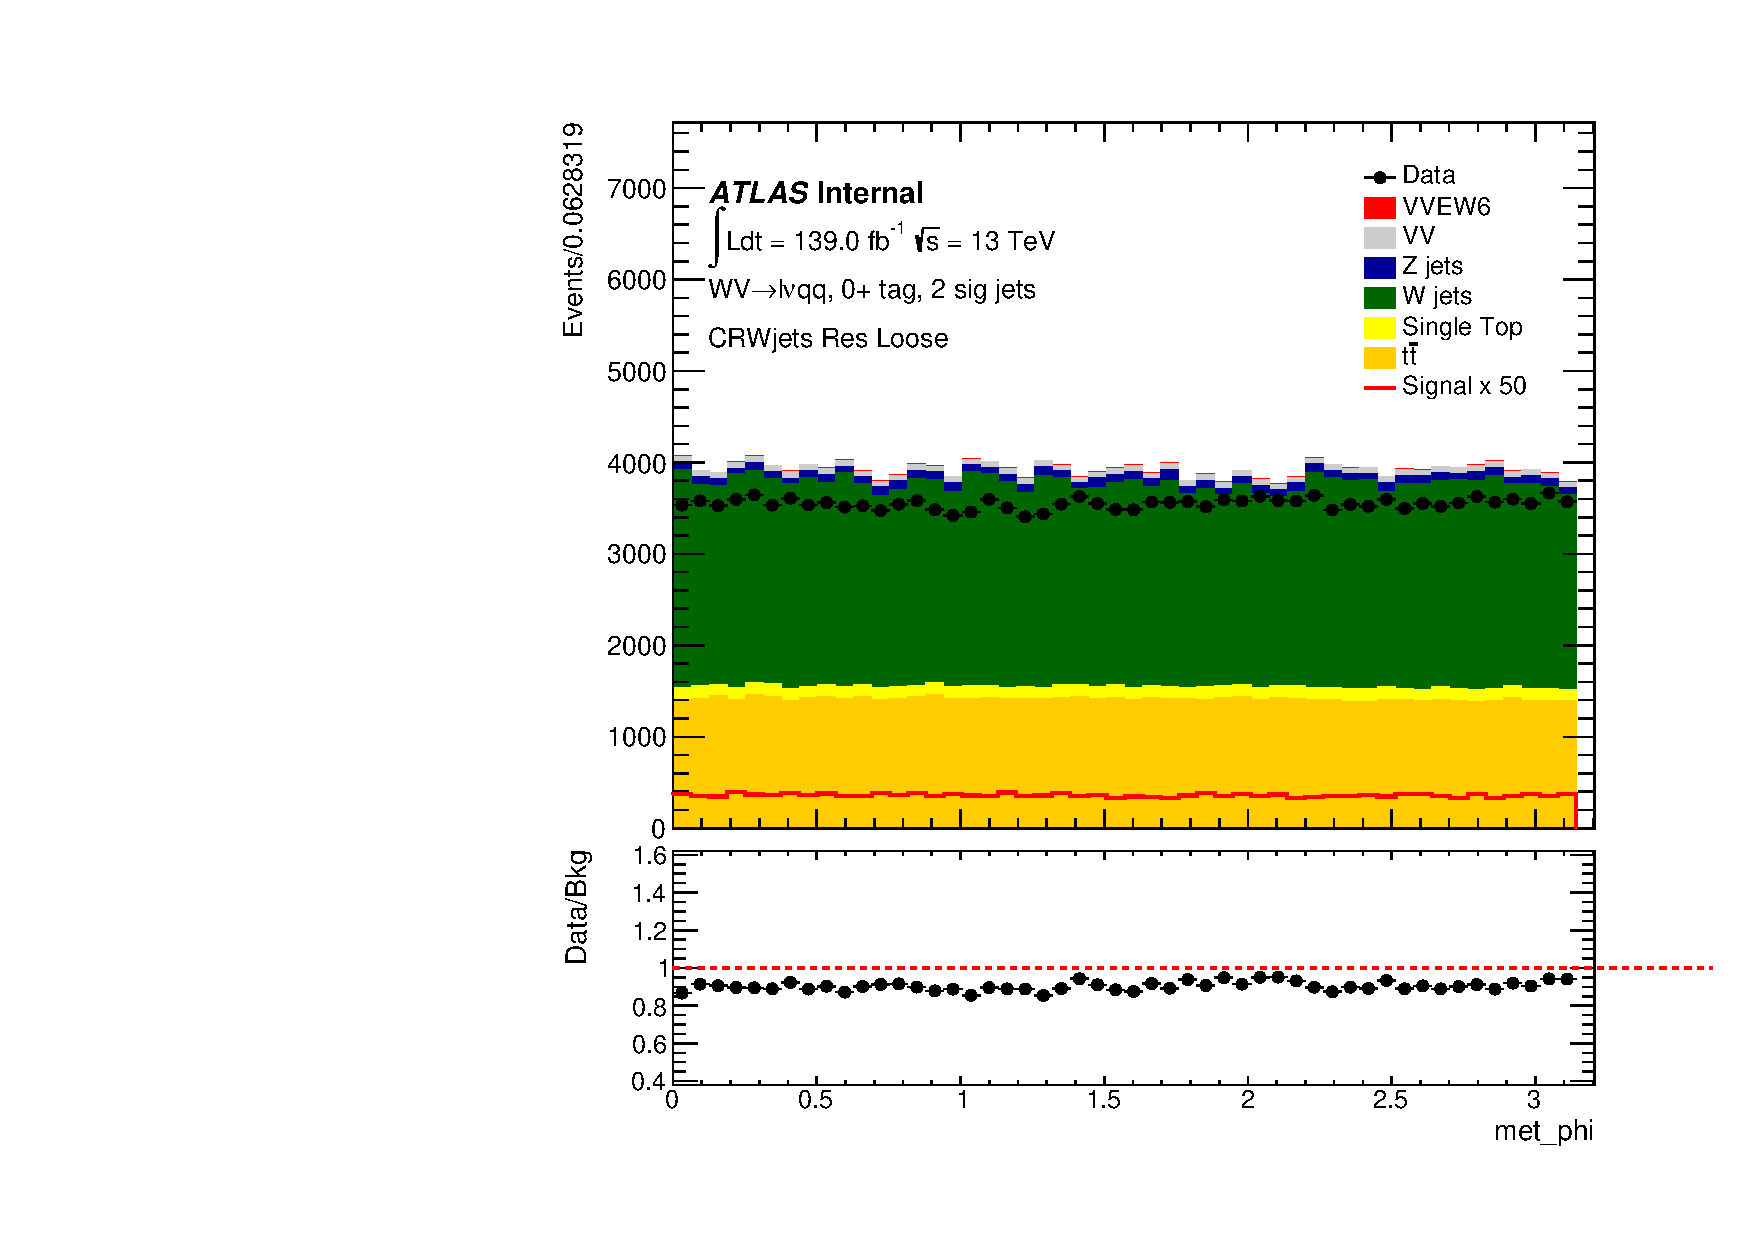
\includegraphics[width=0.3\textwidth]{figures/CRPlots/CRWjets_Res_Loose/stacked_plot_met_phi.pdf}}
%%    \subfloat[]{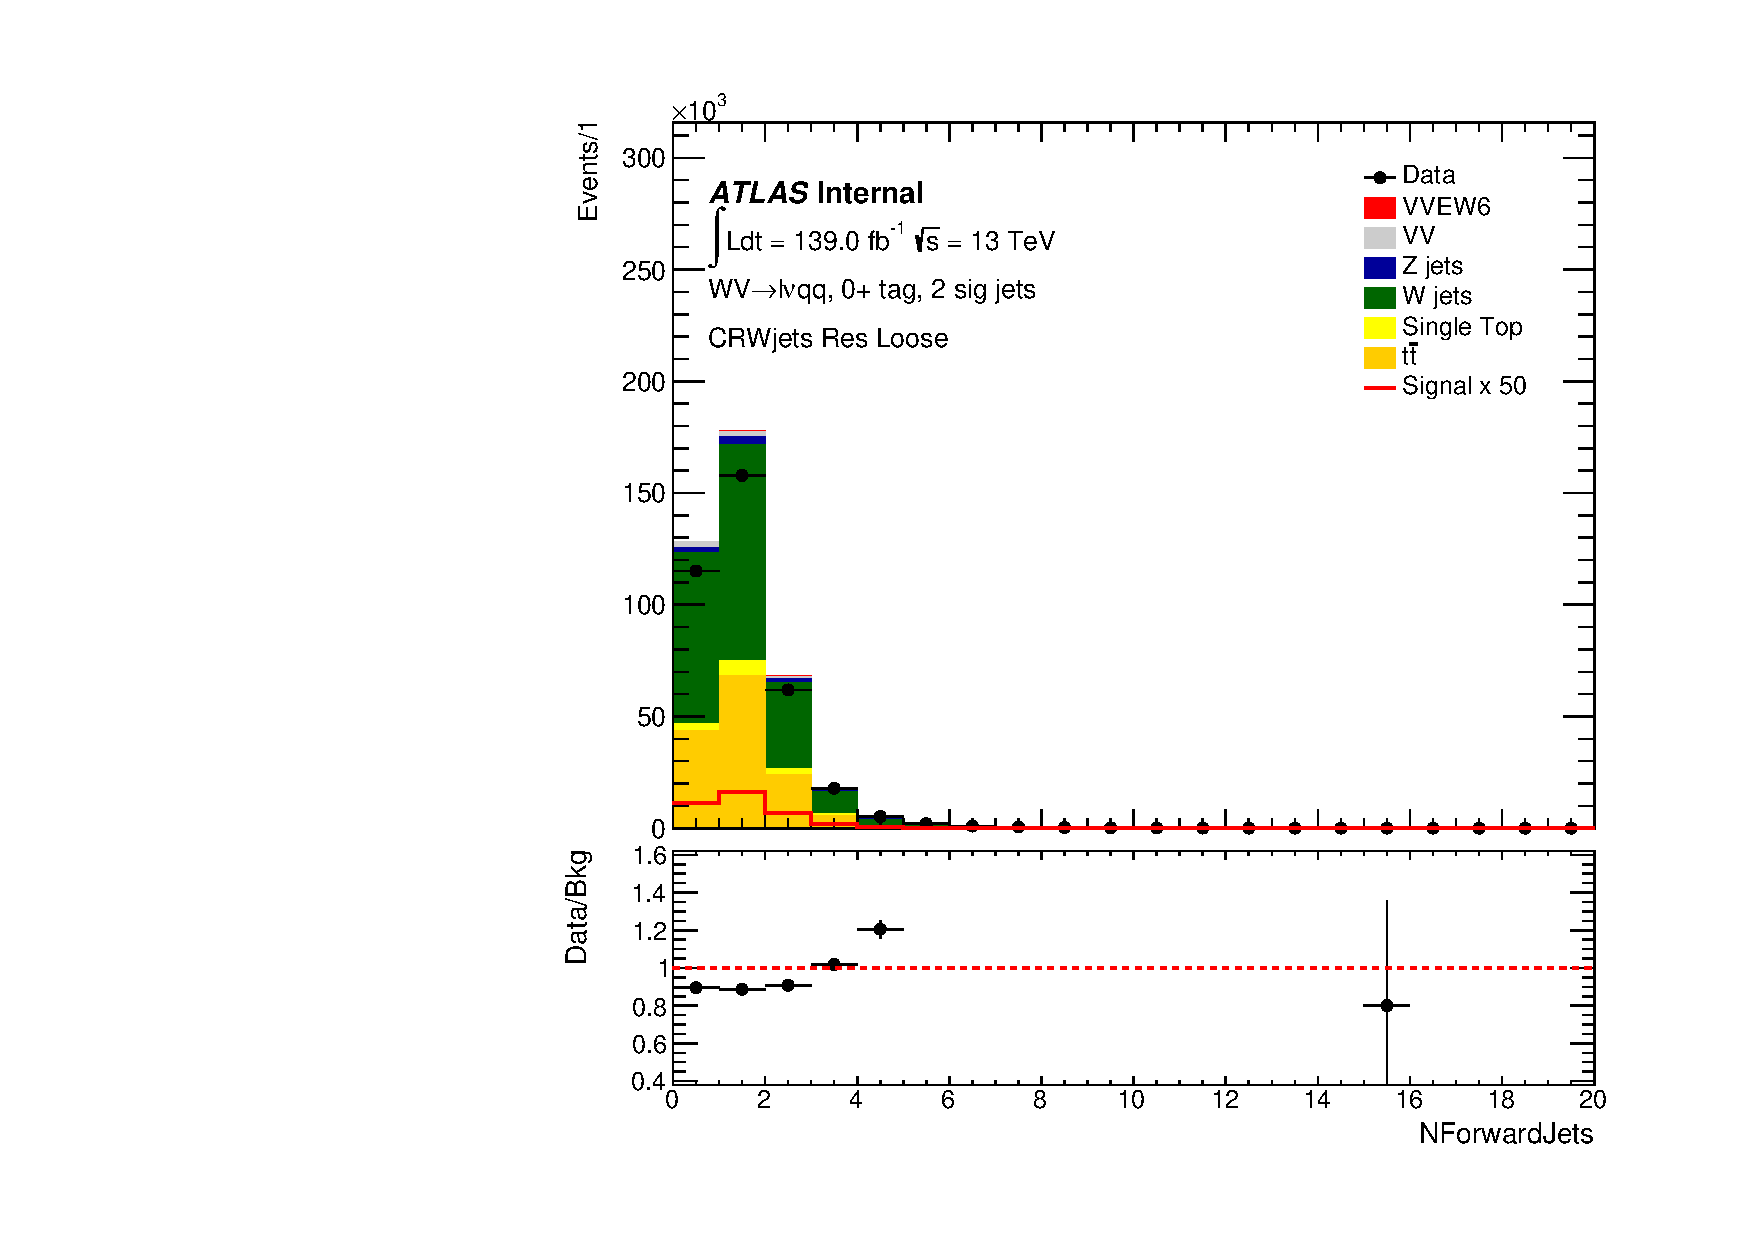
\includegraphics[width=0.3\textwidth]{figures/CRPlots/CRWjets_Res_Loose/stacked_plot_NForwardJets.pdf}}
    \caption{Data-MC checks for the resolved loose \Wjets control region in the \olep channel.}
    \label{fig:CRWjetResLoosePlots1Lep2}
\end{figure}

\begin{figure}[ht]
    \centering
    \subfloat[]{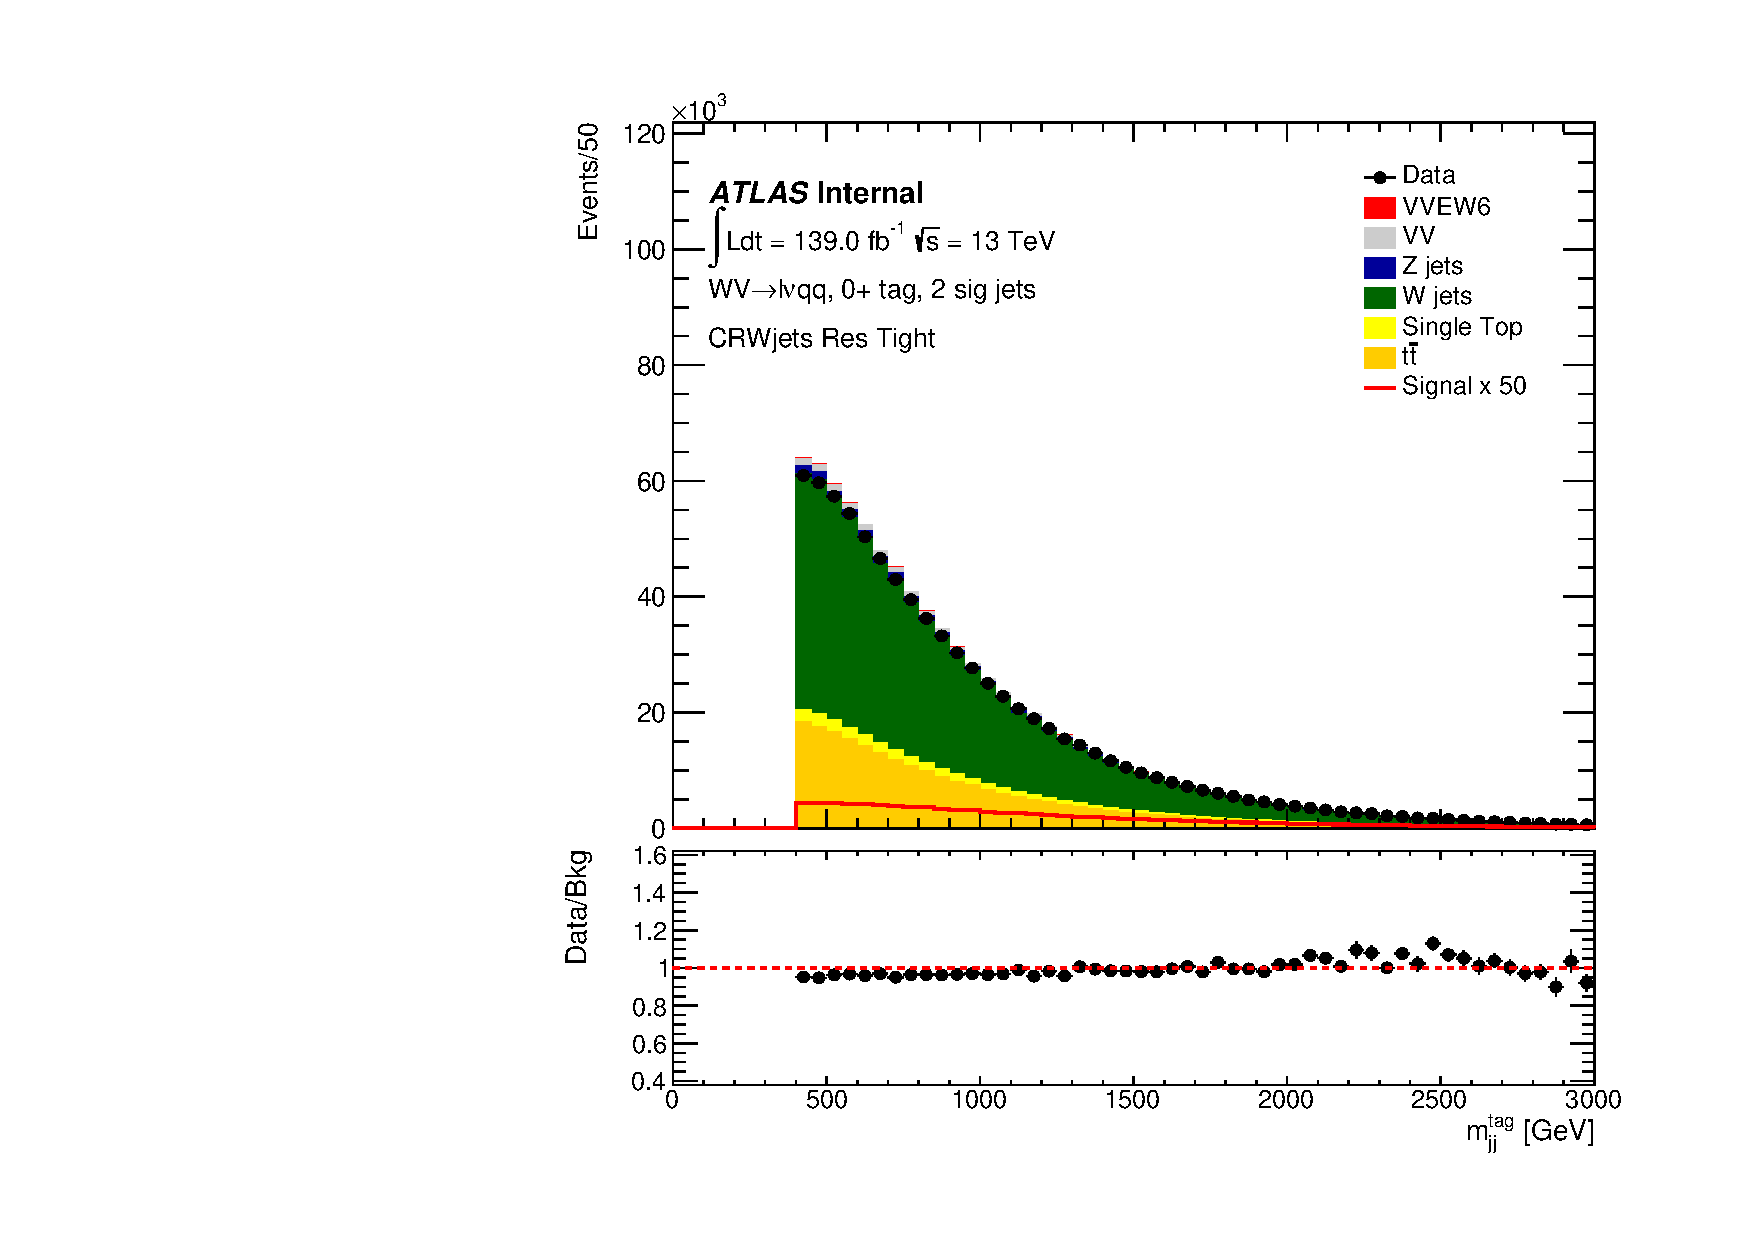
\includegraphics[width=0.3\textwidth]{figures/CRPlots/CRWjets_Res_Tight/stacked_plot_resolved_tagMjj.pdf}}
    \subfloat[]{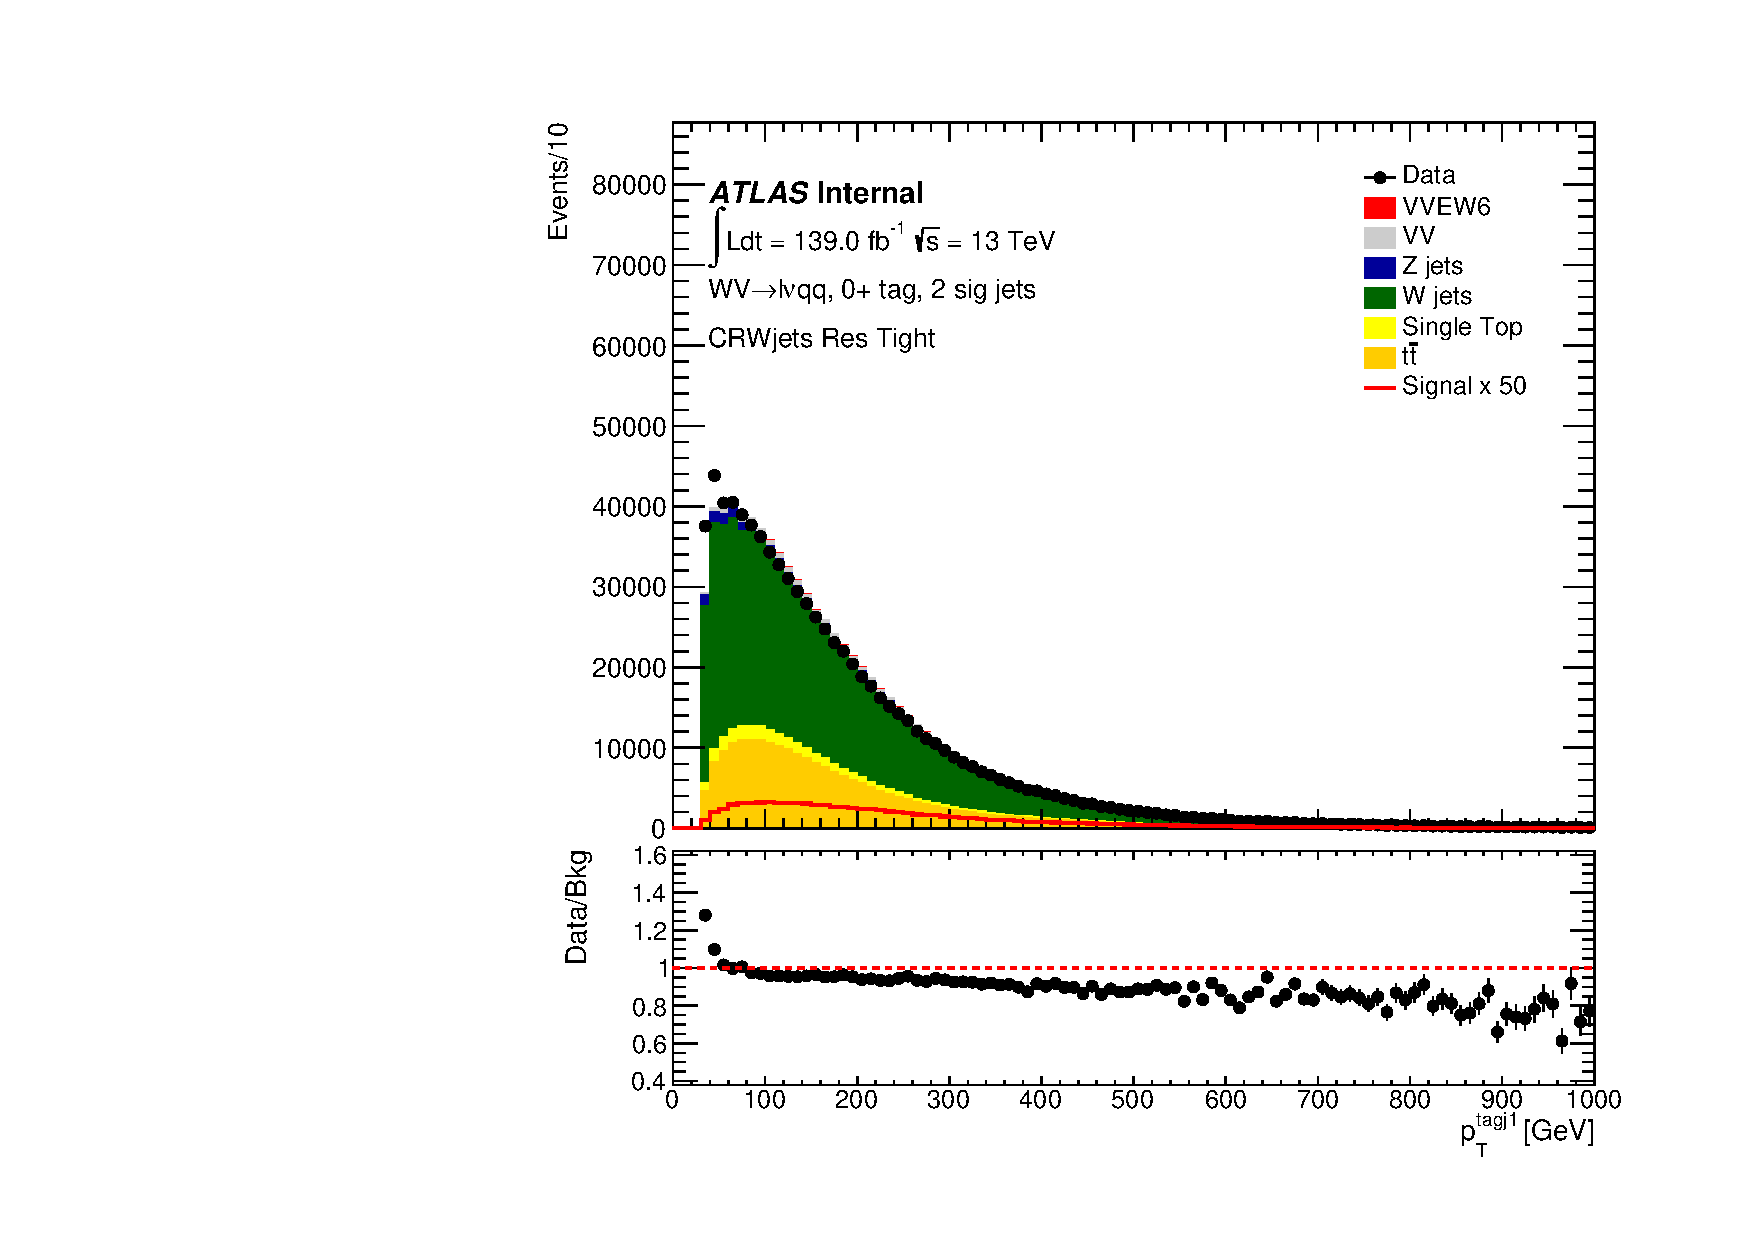
\includegraphics[width=0.3\textwidth]{figures/CRPlots/CRWjets_Res_Tight/stacked_plot_resolved_tagJ1_pt.pdf}}
    \subfloat[]{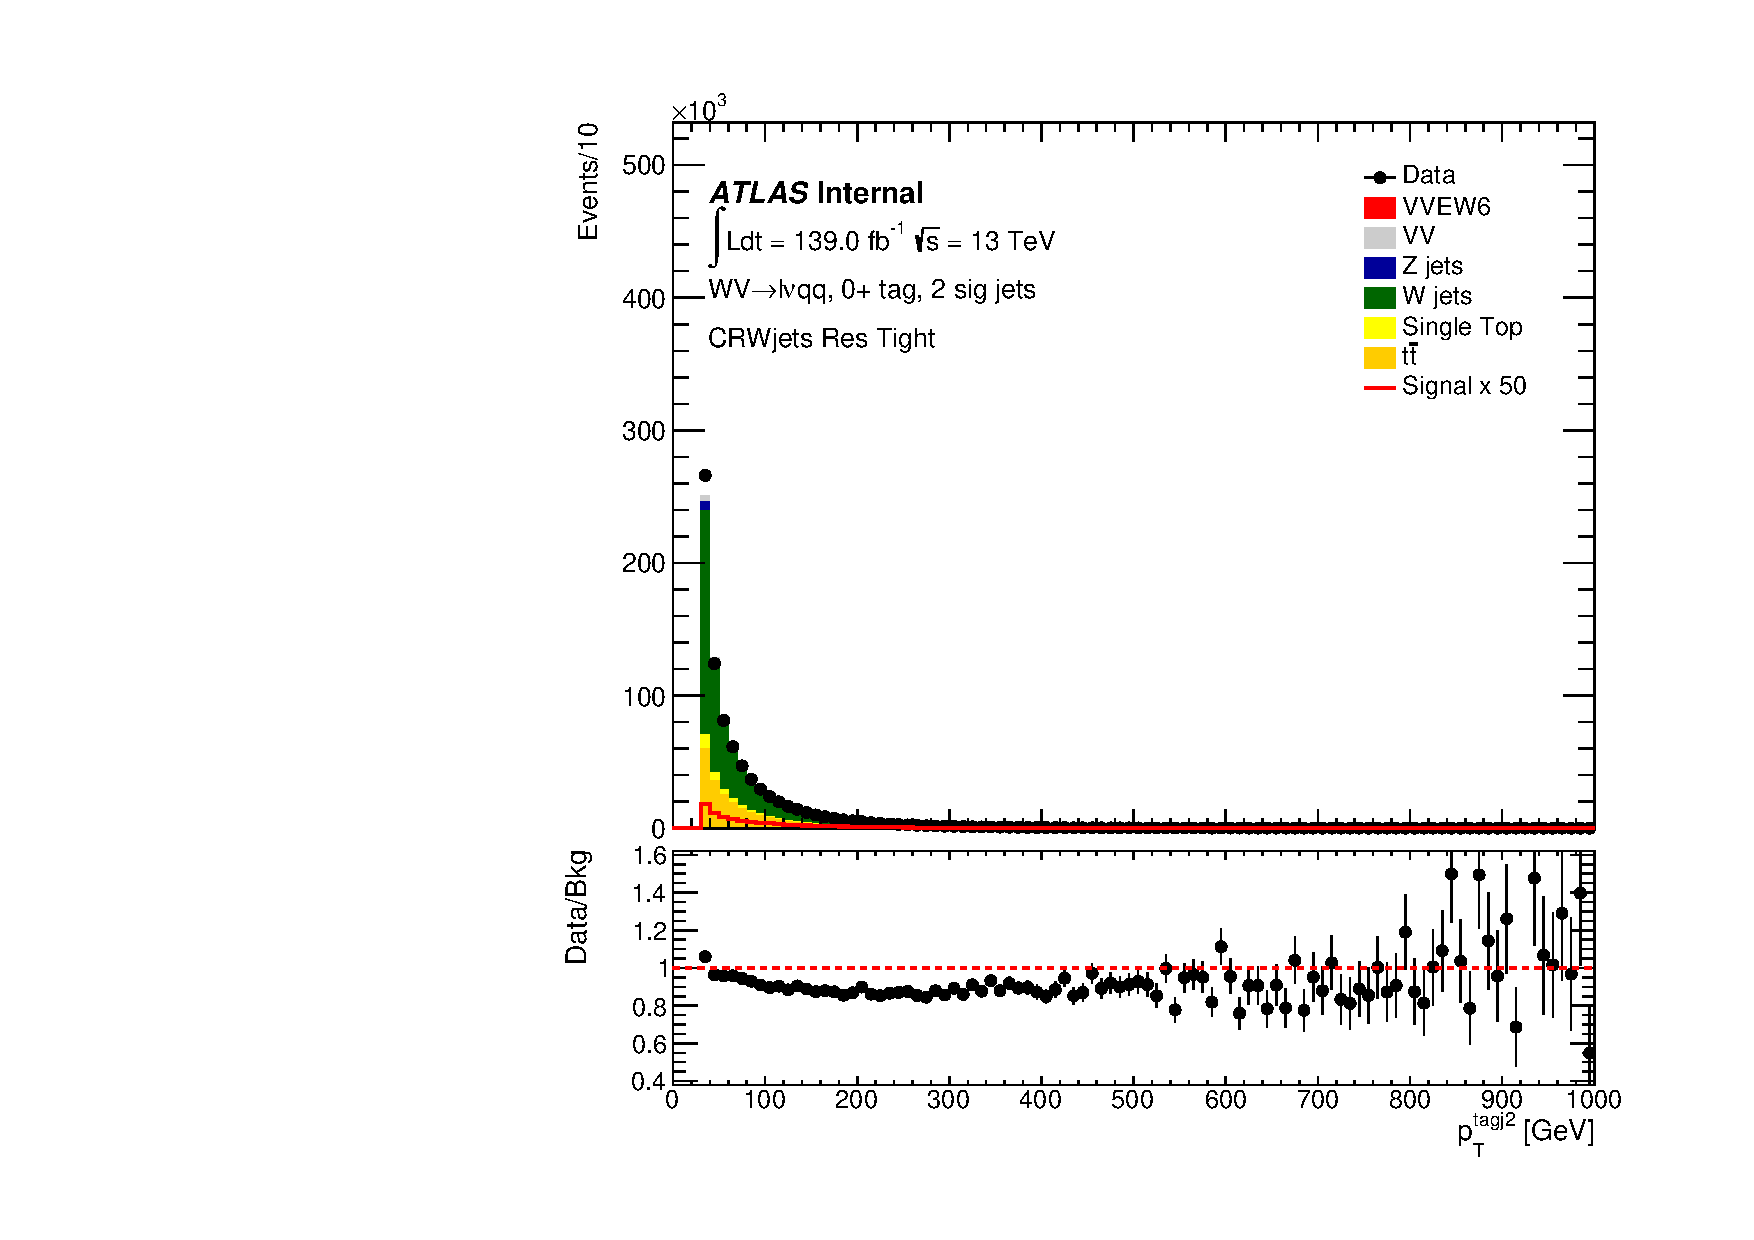
\includegraphics[width=0.3\textwidth]{figures/CRPlots/CRWjets_Res_Tight/stacked_plot_resolved_tagJ2_pt.pdf}} \\
    \subfloat[]{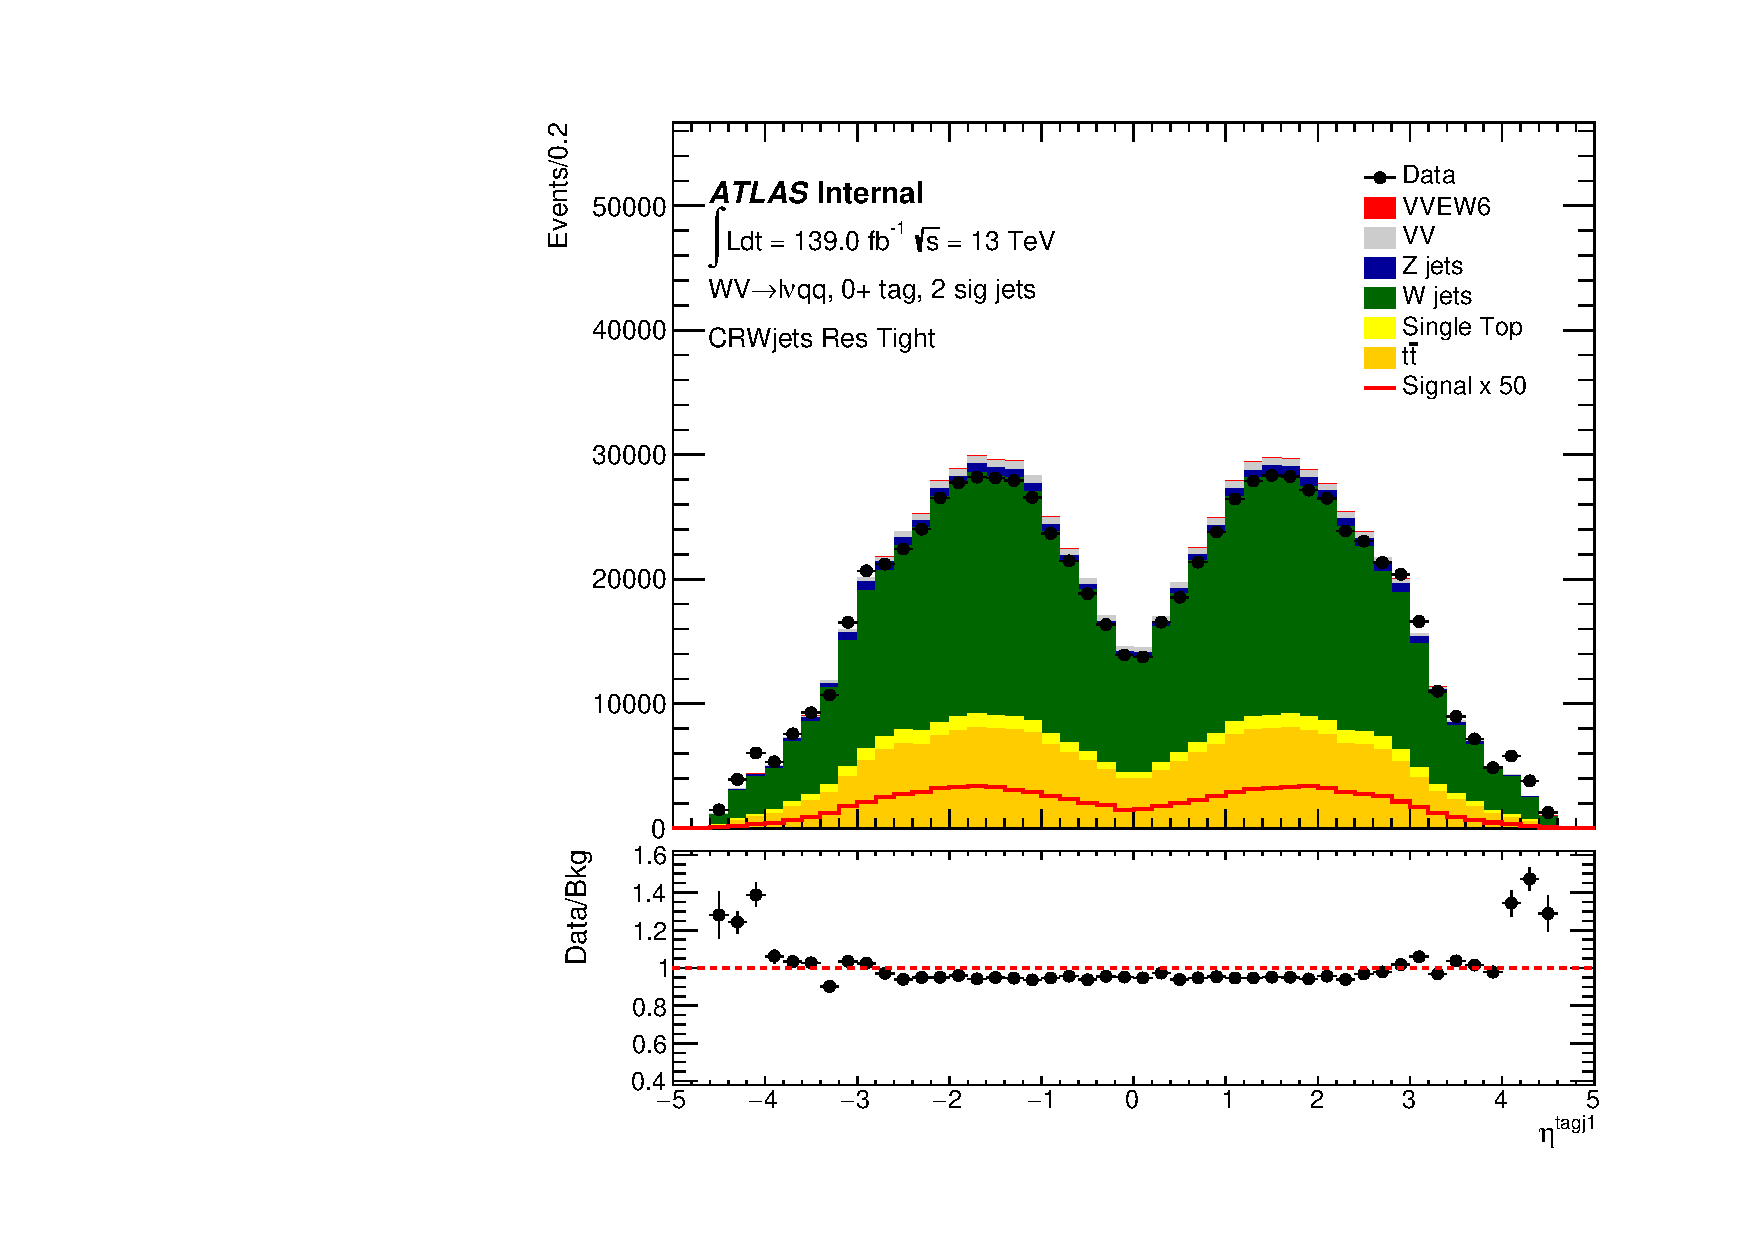
\includegraphics[width=0.3\textwidth]{figures/CRPlots/CRWjets_Res_Tight/stacked_plot_resolved_tagJ1_eta.pdf}}
    \subfloat[]{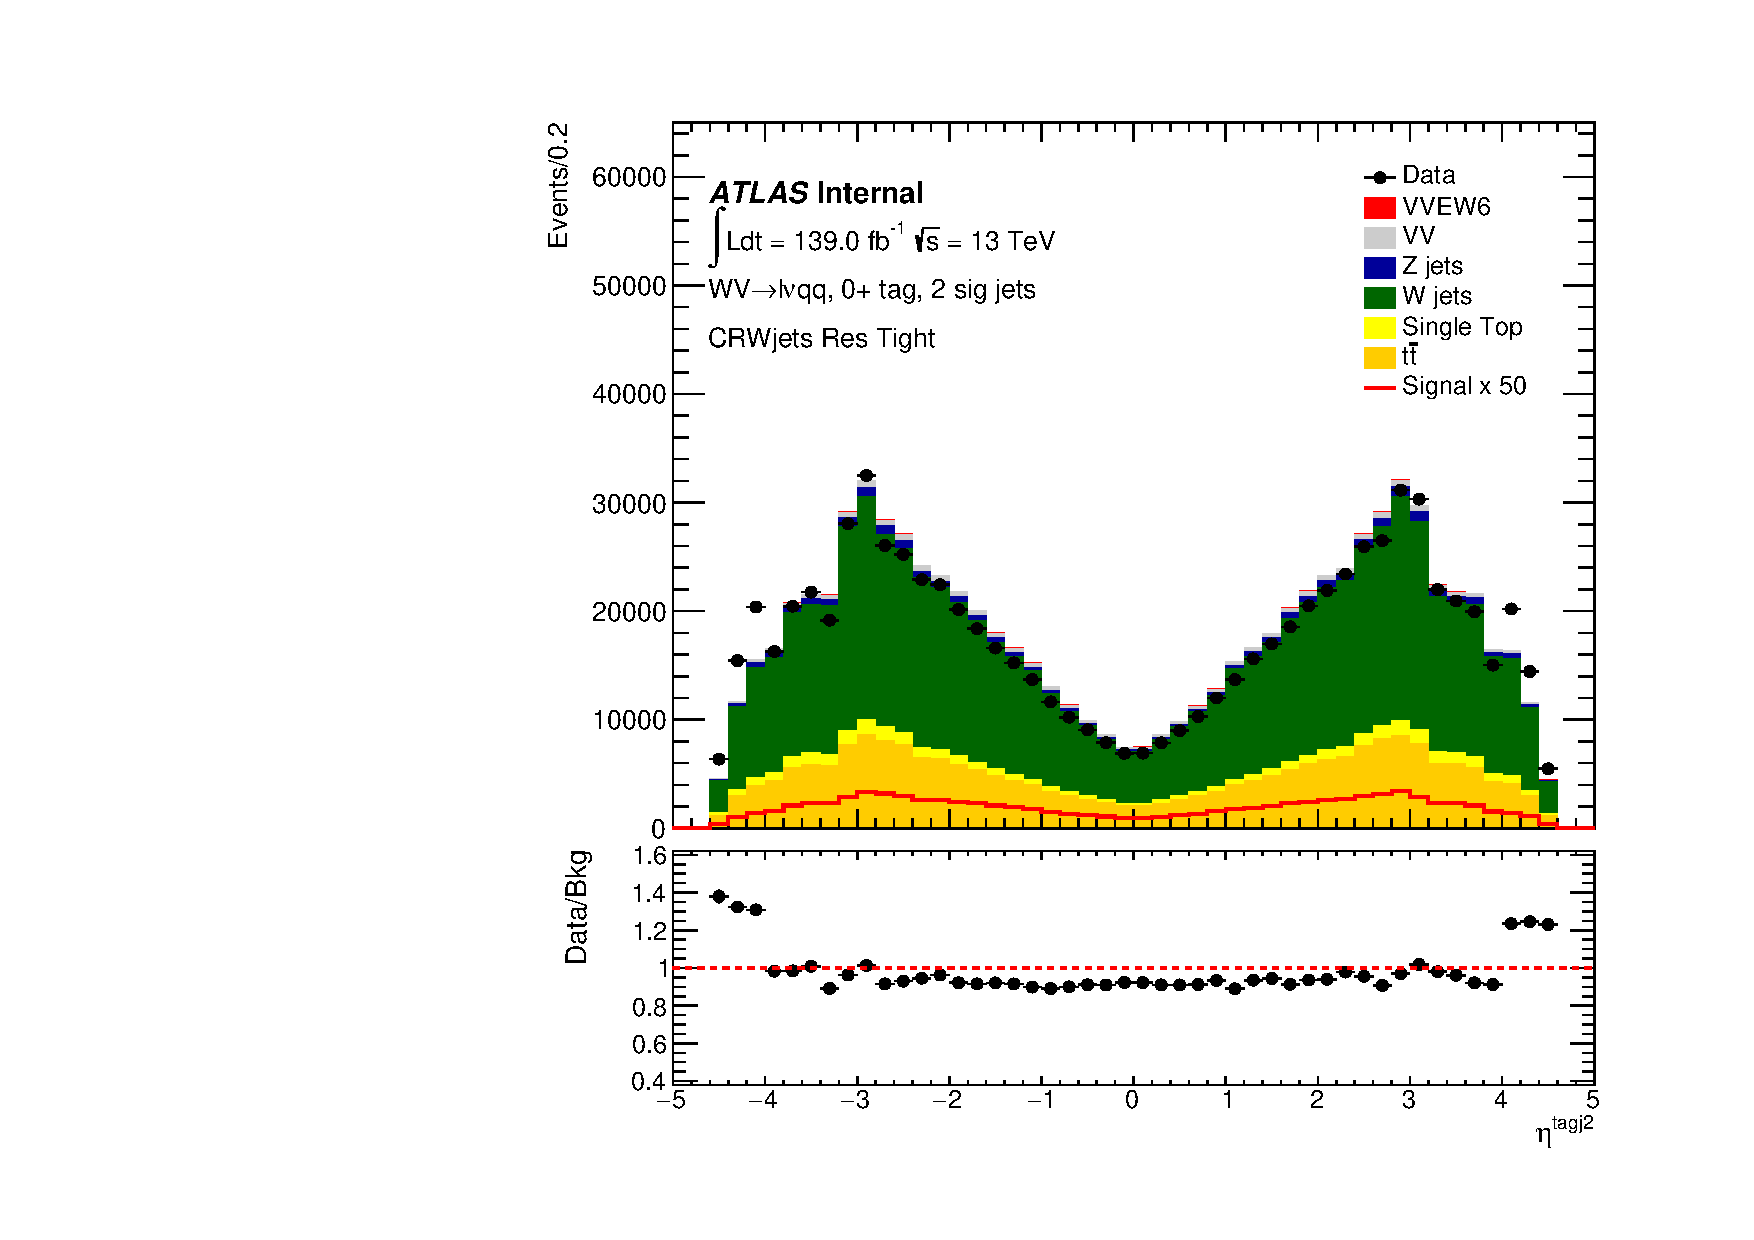
\includegraphics[width=0.3\textwidth]{figures/CRPlots/CRWjets_Res_Tight/stacked_plot_resolved_tagJ2_eta.pdf}} \\
    \subfloat[]{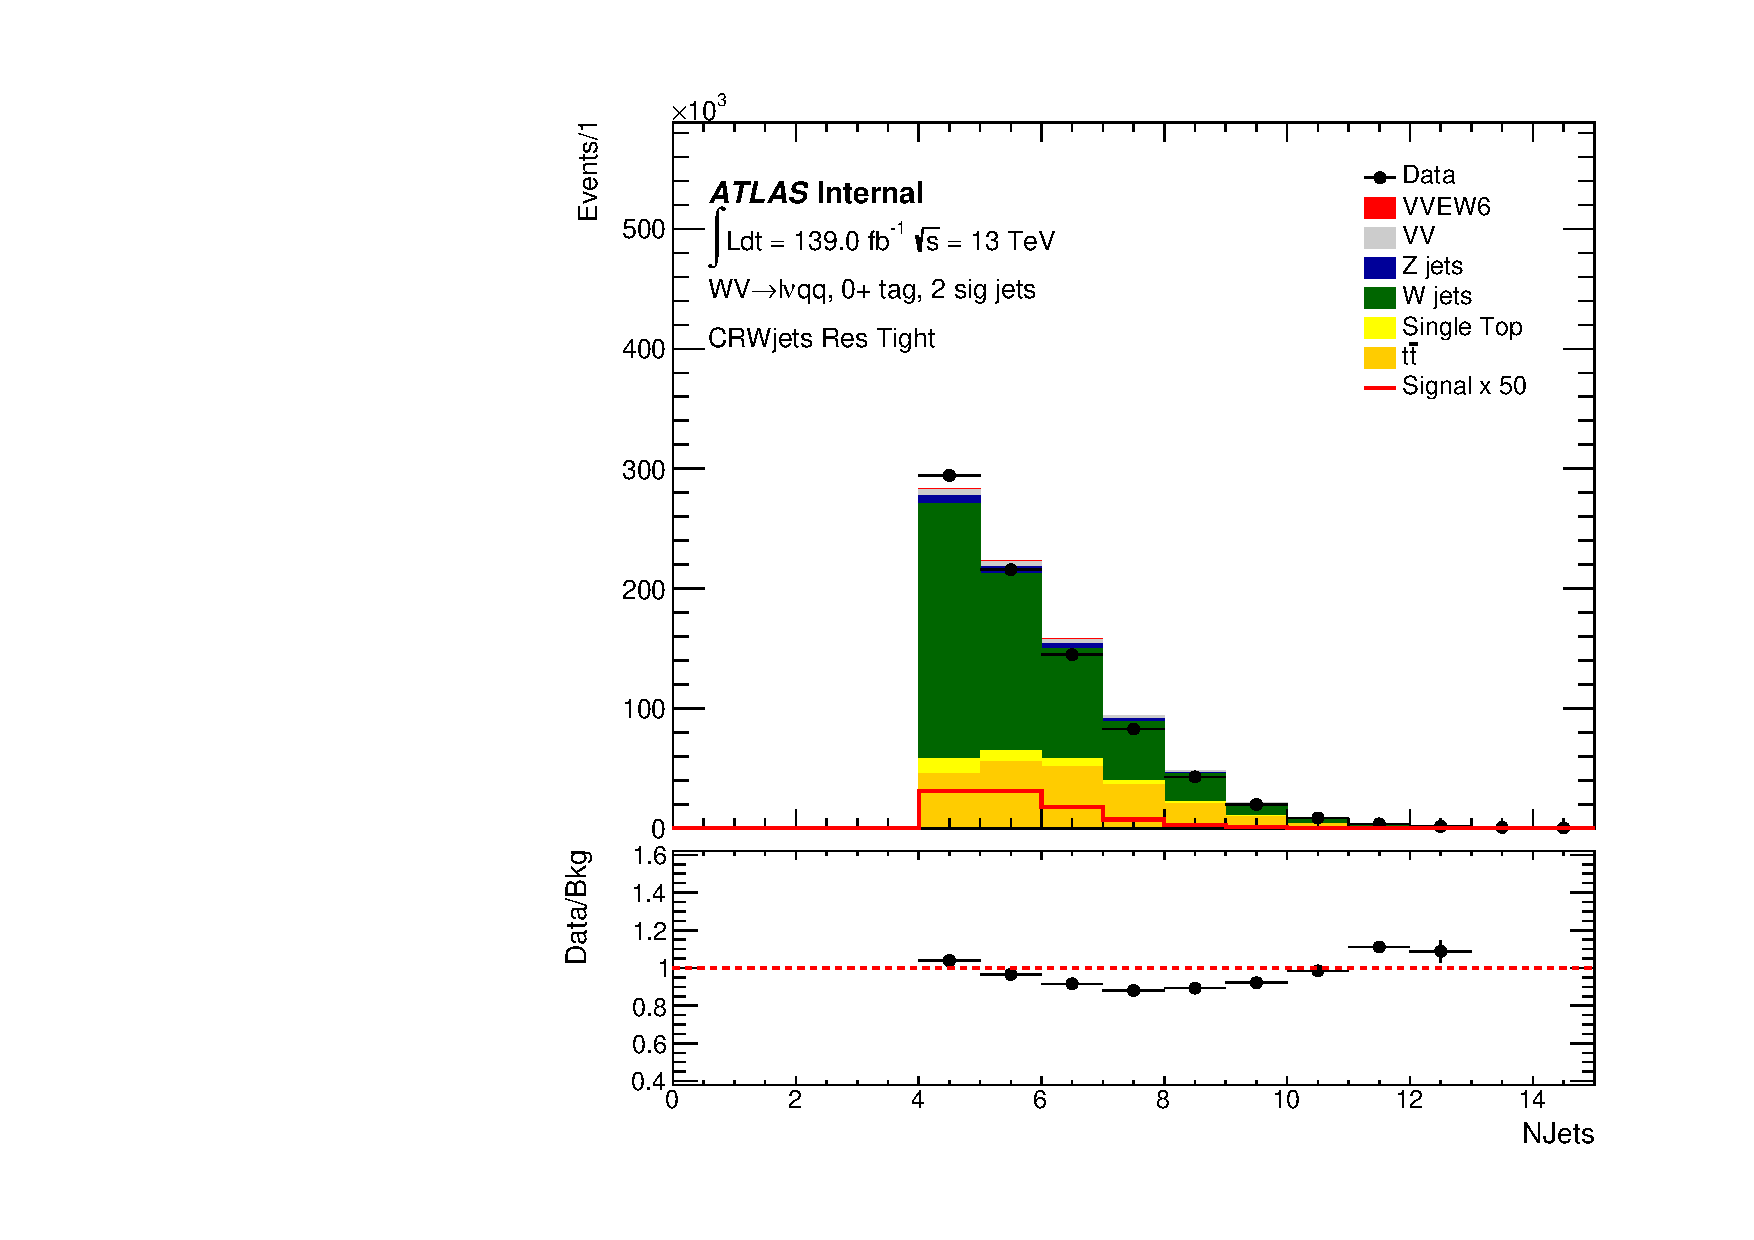
\includegraphics[width=0.3\textwidth]{figures/CRPlots/CRWjets_Res_Tight/stacked_plot_NJets.pdf}}
    \subfloat[]{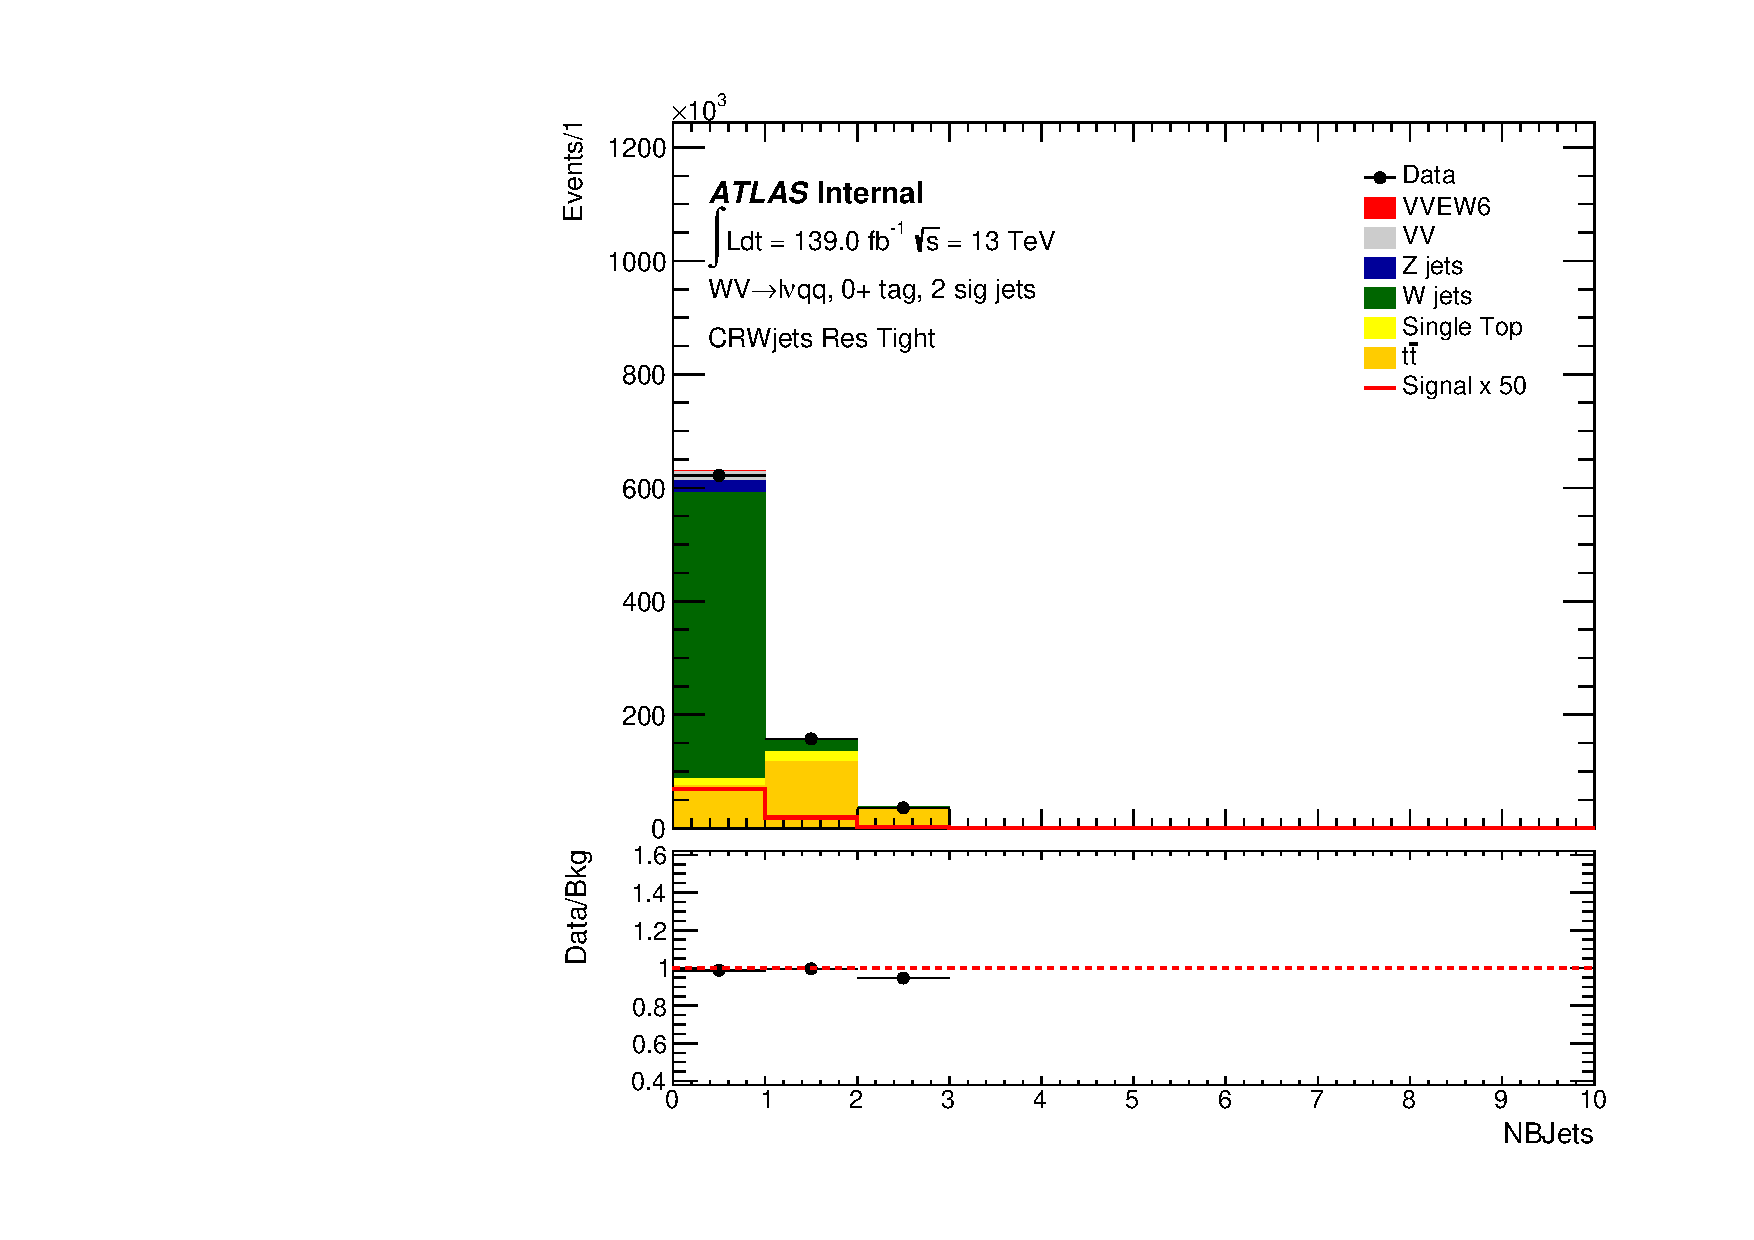
\includegraphics[width=0.3\textwidth]{figures/CRPlots/CRWjets_Res_Tight/stacked_plot_NBJets.pdf}}
    \subfloat[]{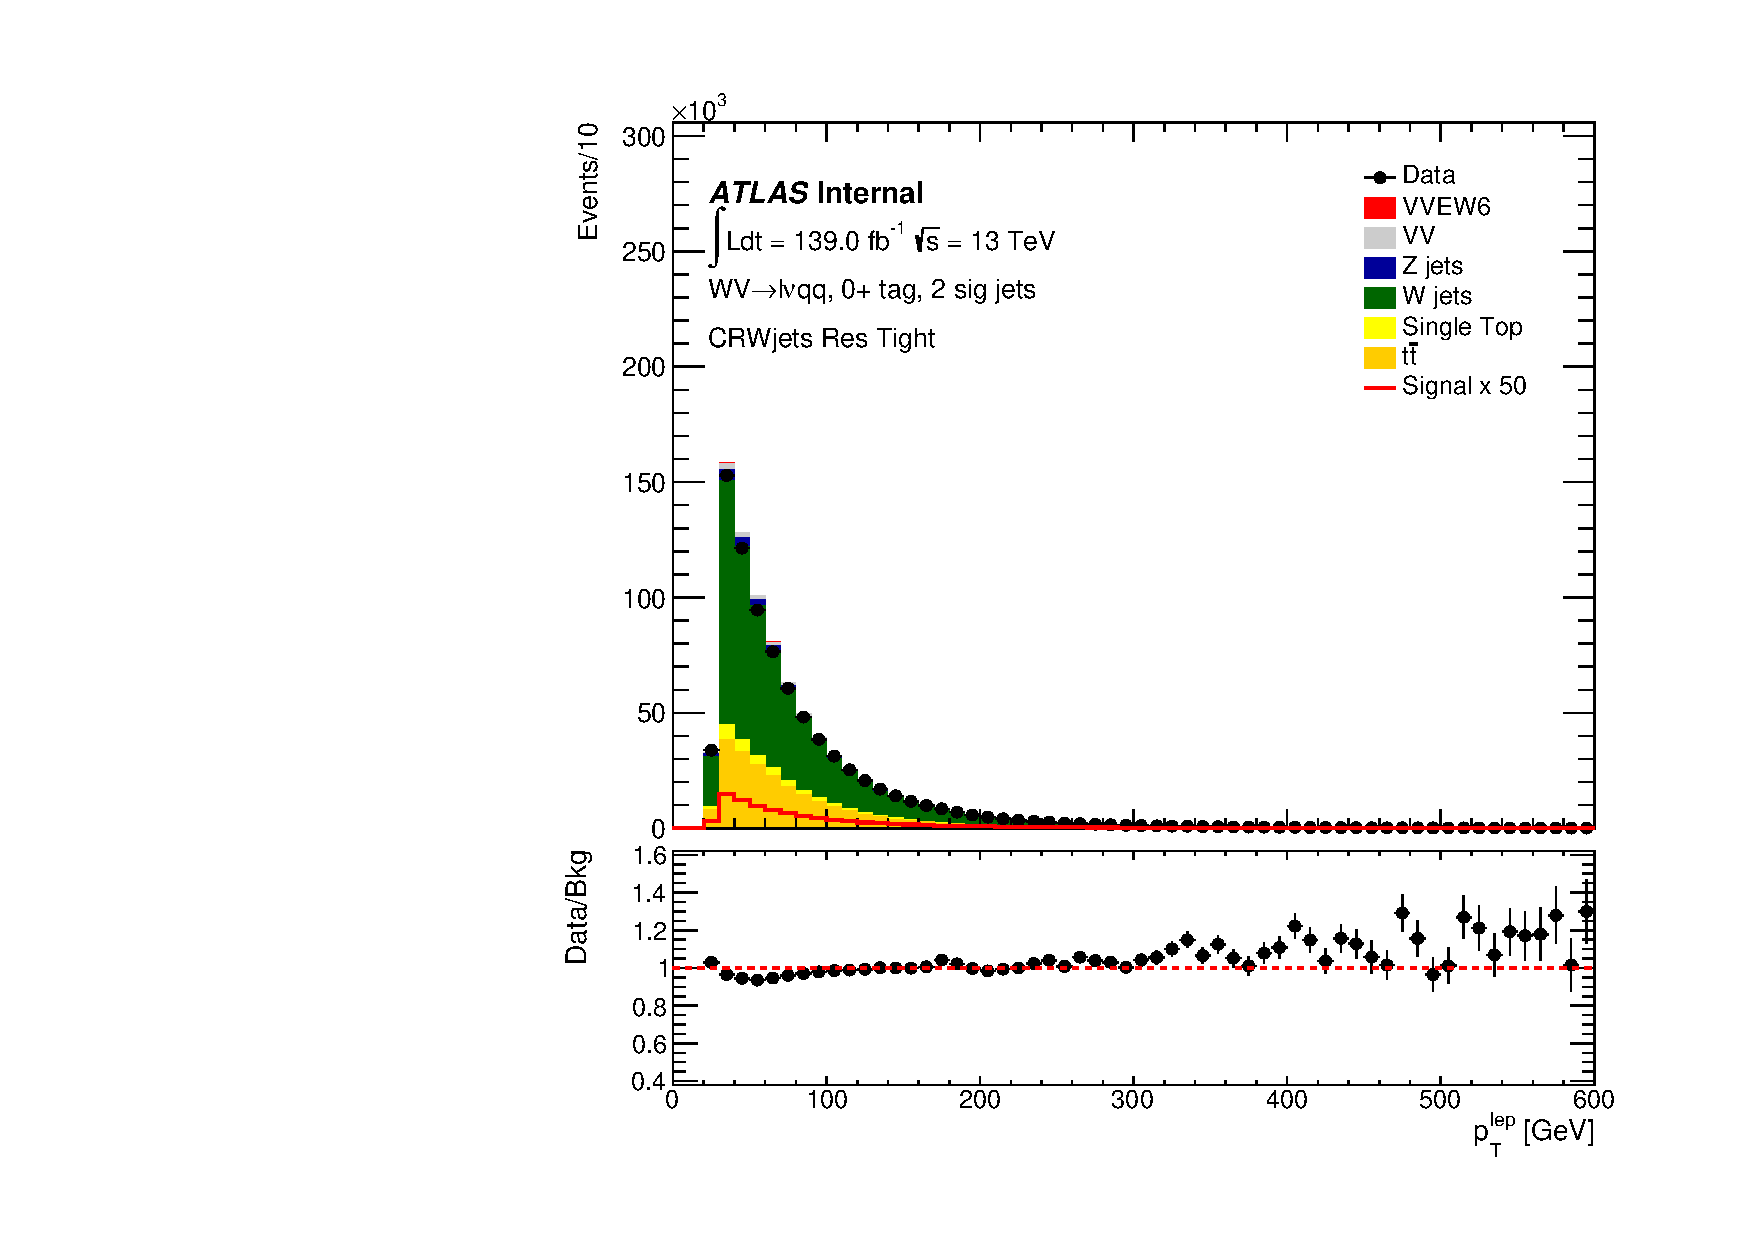
\includegraphics[width=0.3\textwidth]{figures/CRPlots/CRWjets_Res_Tight/stacked_plot_lep_pt.pdf}}  %%\\
    \caption{Data-MC checks for the resolved tight \Wjets control region in the \olep channel.}
    \label{fig:CRWjetResTightPlots1Lep}
\end{figure}


\begin{figure}[ht]
    \centering
    \subfloat[]{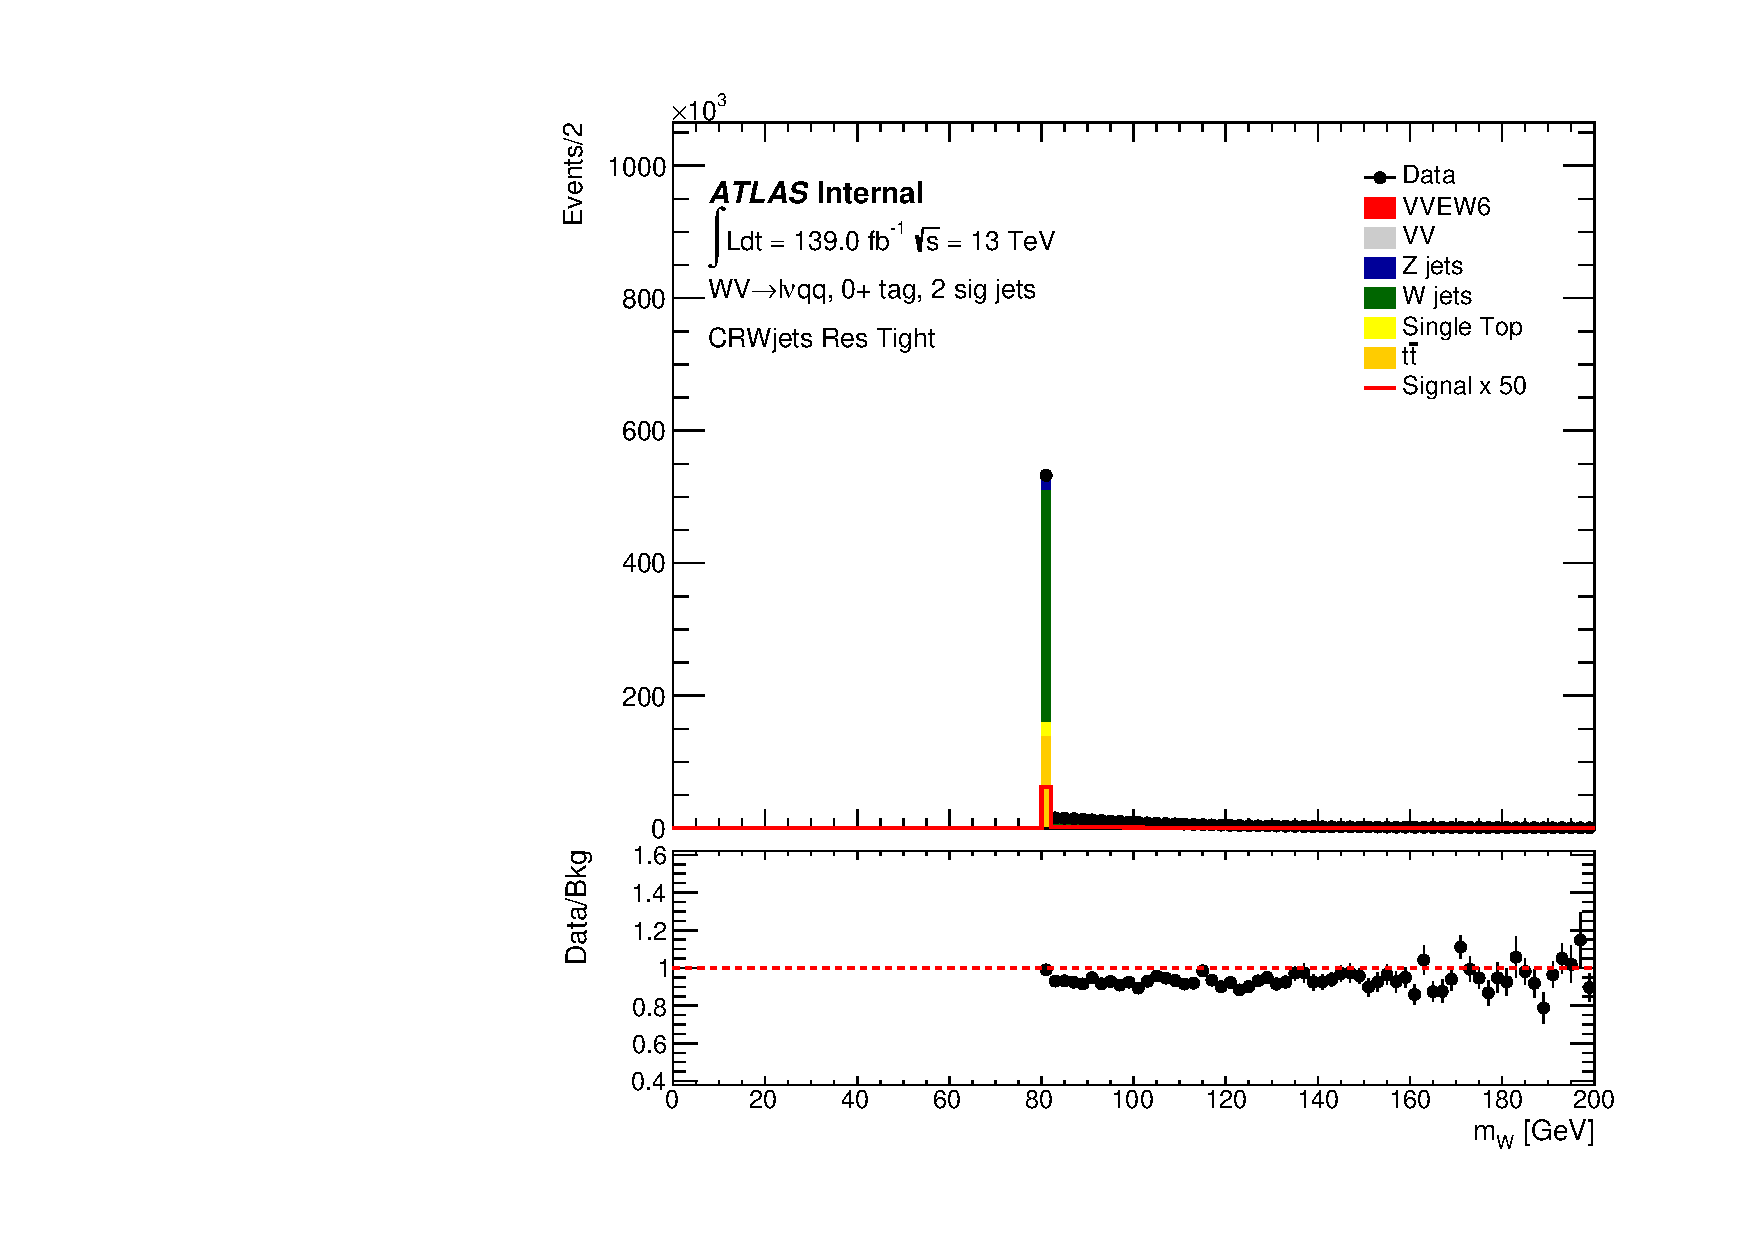
\includegraphics[width=0.3\textwidth]{figures/CRPlots/CRWjets_Res_Tight/stacked_plot_W_m.pdf}}
    \subfloat[]{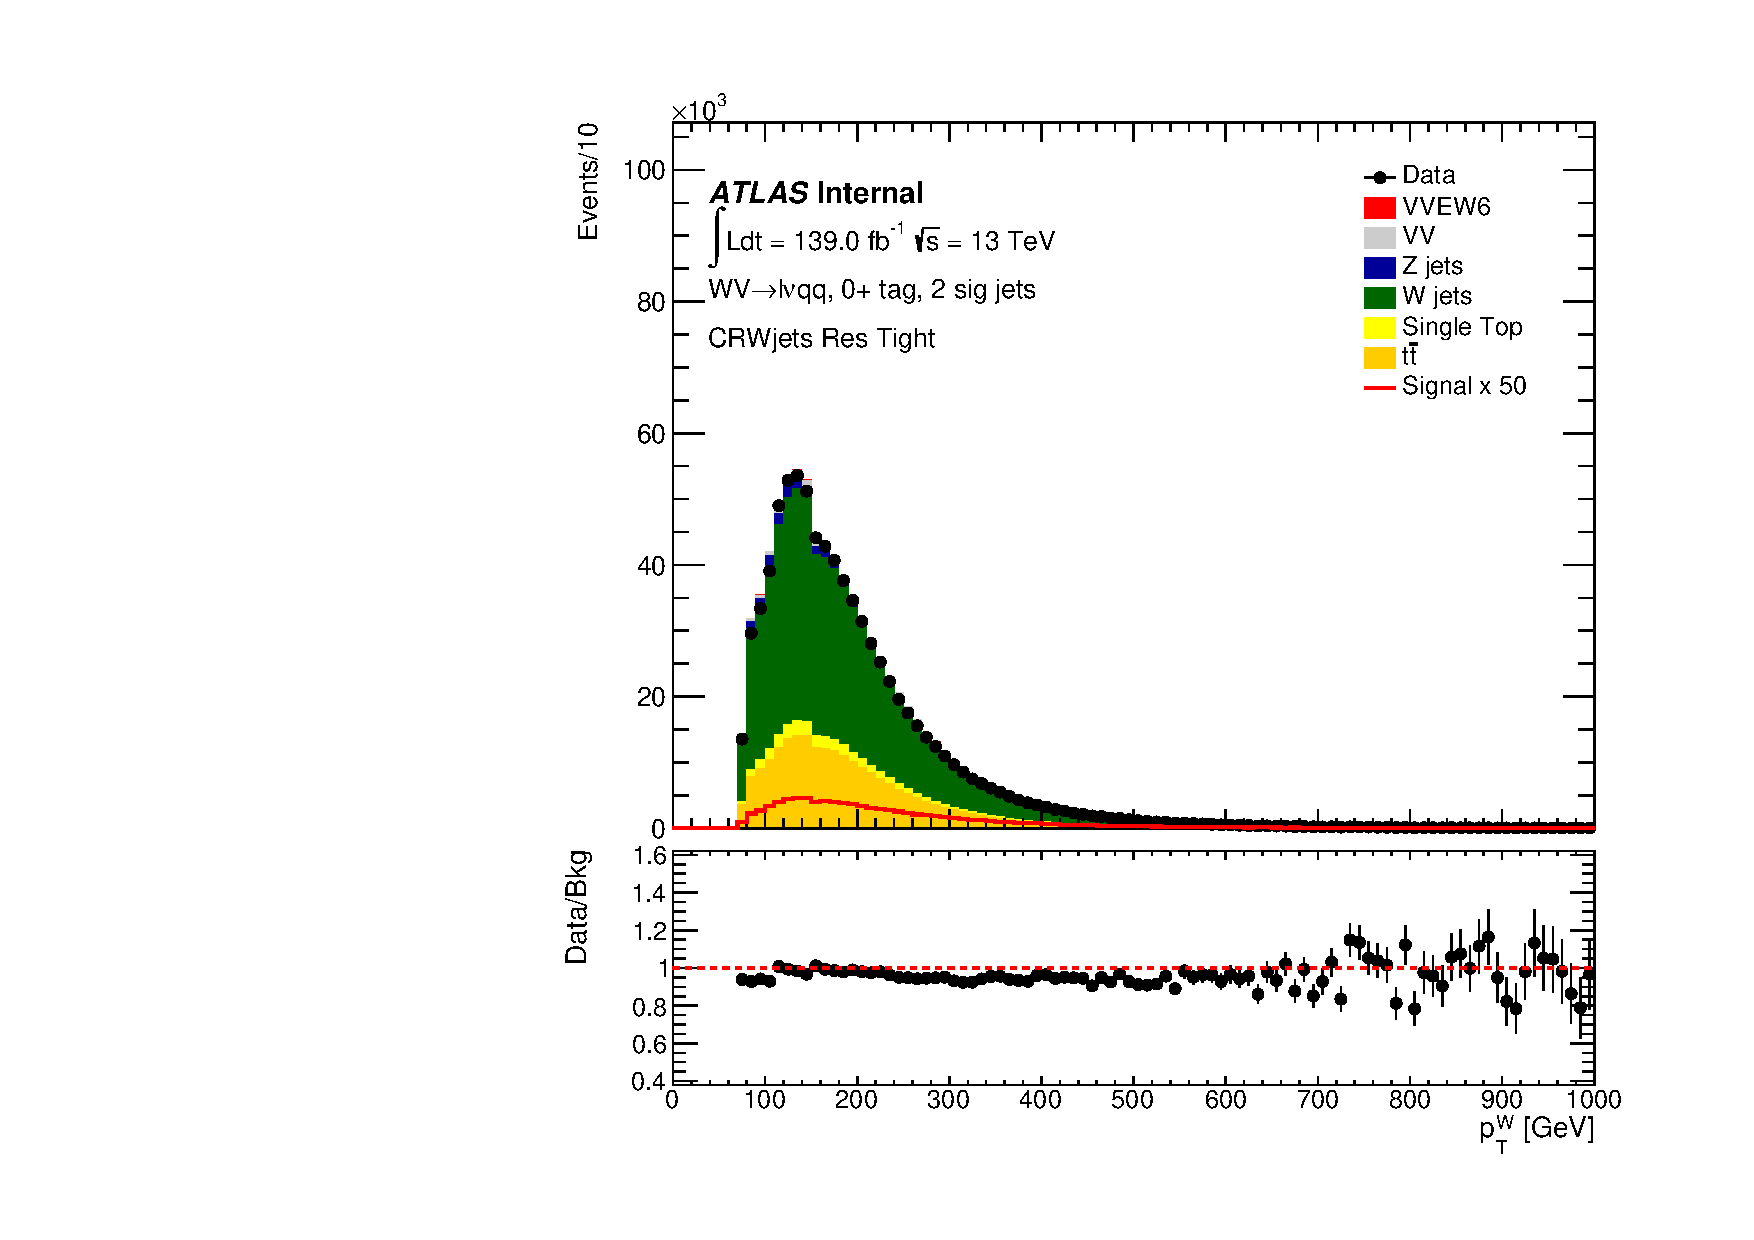
\includegraphics[width=0.3\textwidth]{figures/CRPlots/CRWjets_Res_Tight/stacked_plot_W_pt.pdf}}
    \subfloat[]{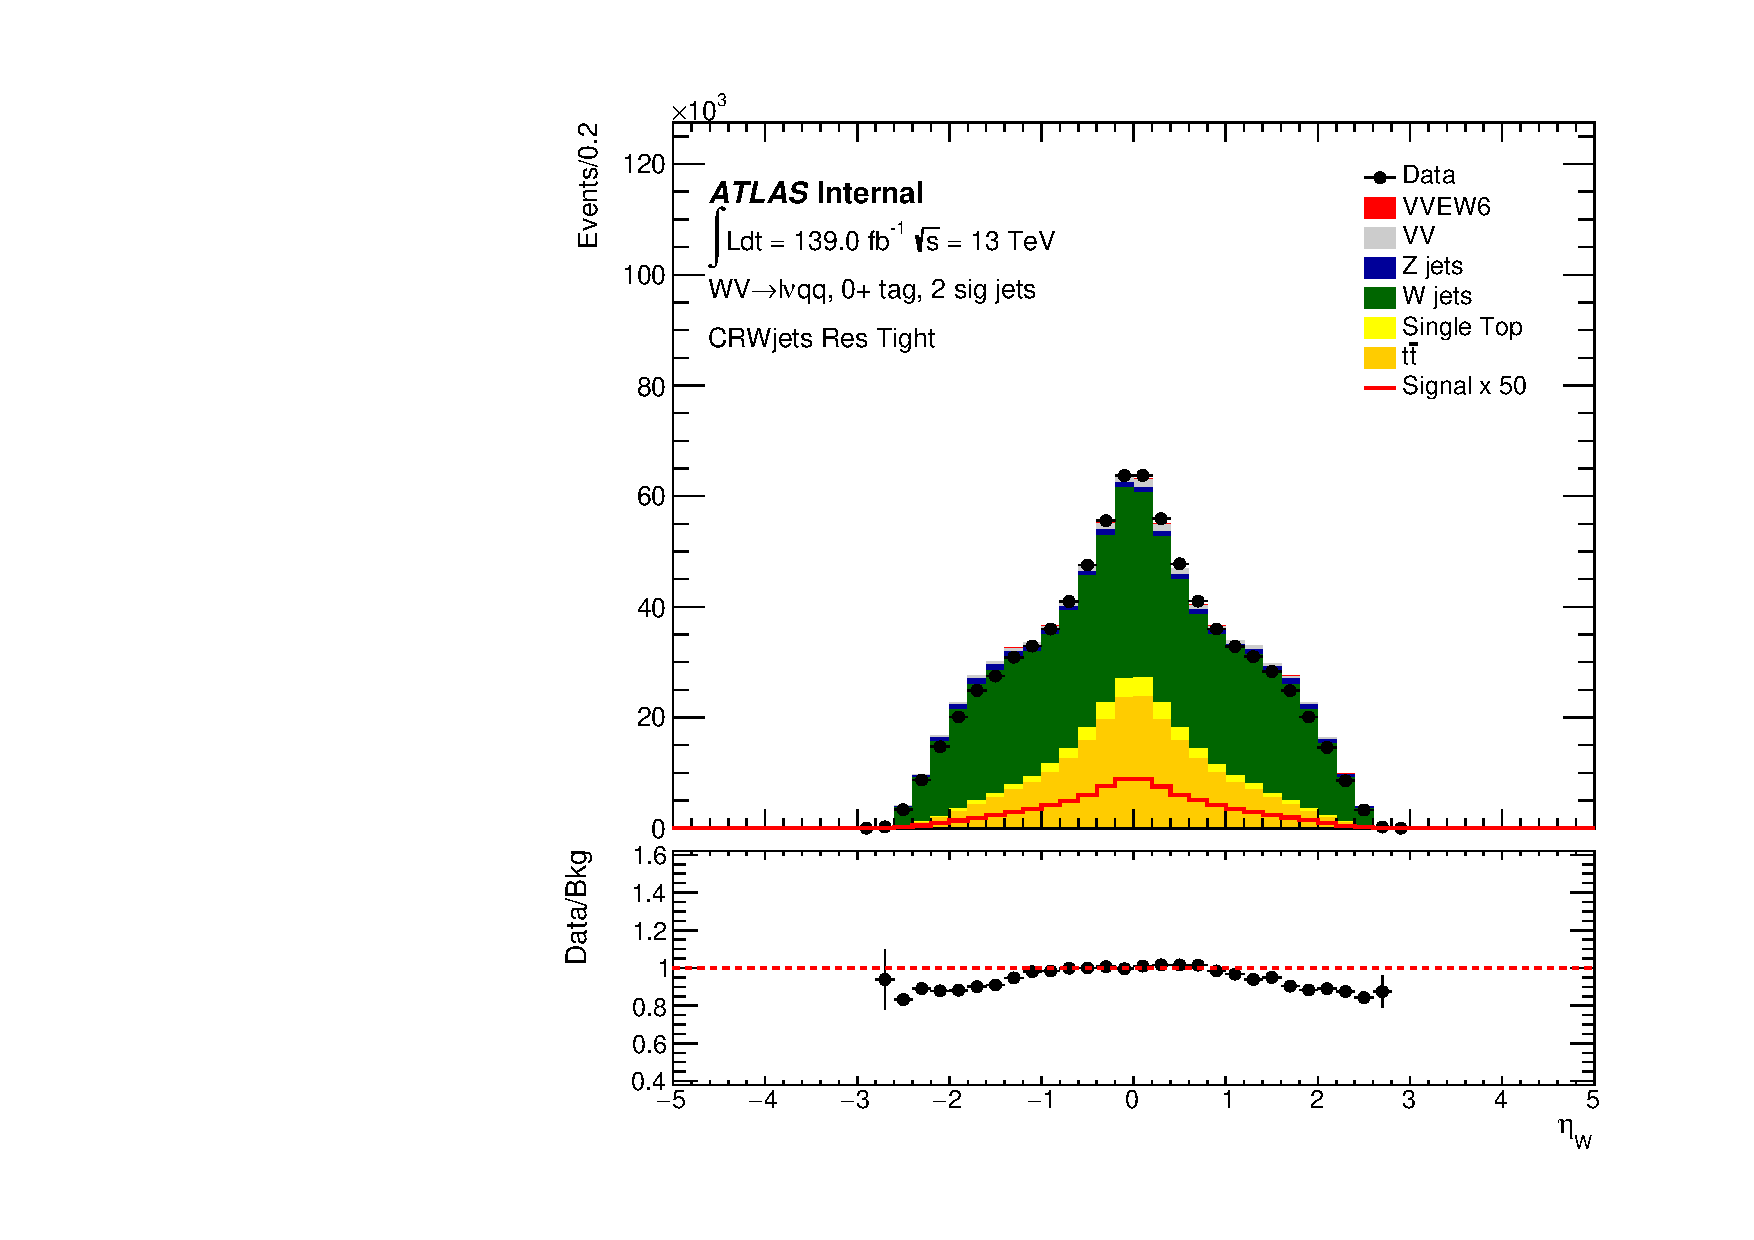
\includegraphics[width=0.3\textwidth]{figures/CRPlots/CRWjets_Res_Tight/stacked_plot_W_eta.pdf}} \\
    \subfloat[]{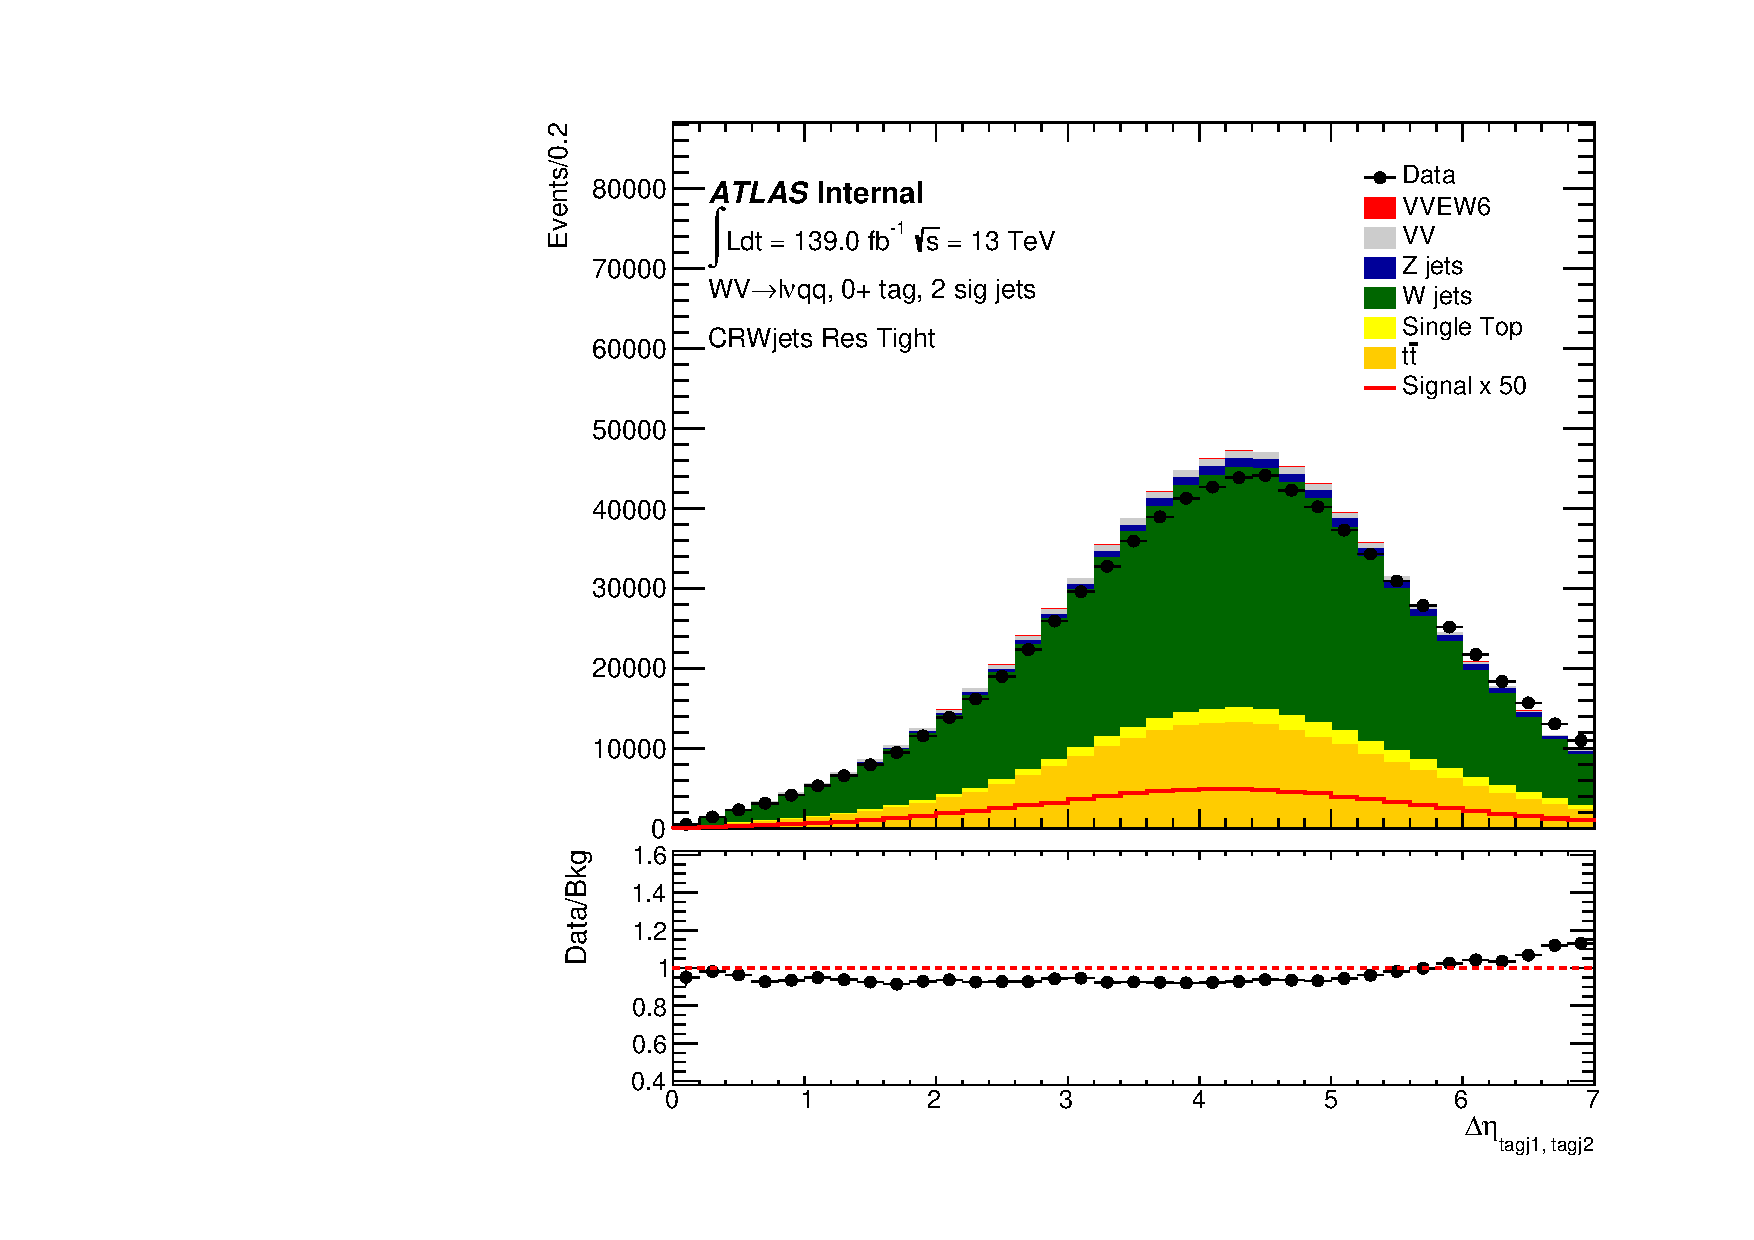
\includegraphics[width=0.3\textwidth]{figures/CRPlots/CRWjets_Res_Tight/stacked_plot_resolved_tagJdEta.pdf}}
    \subfloat[]{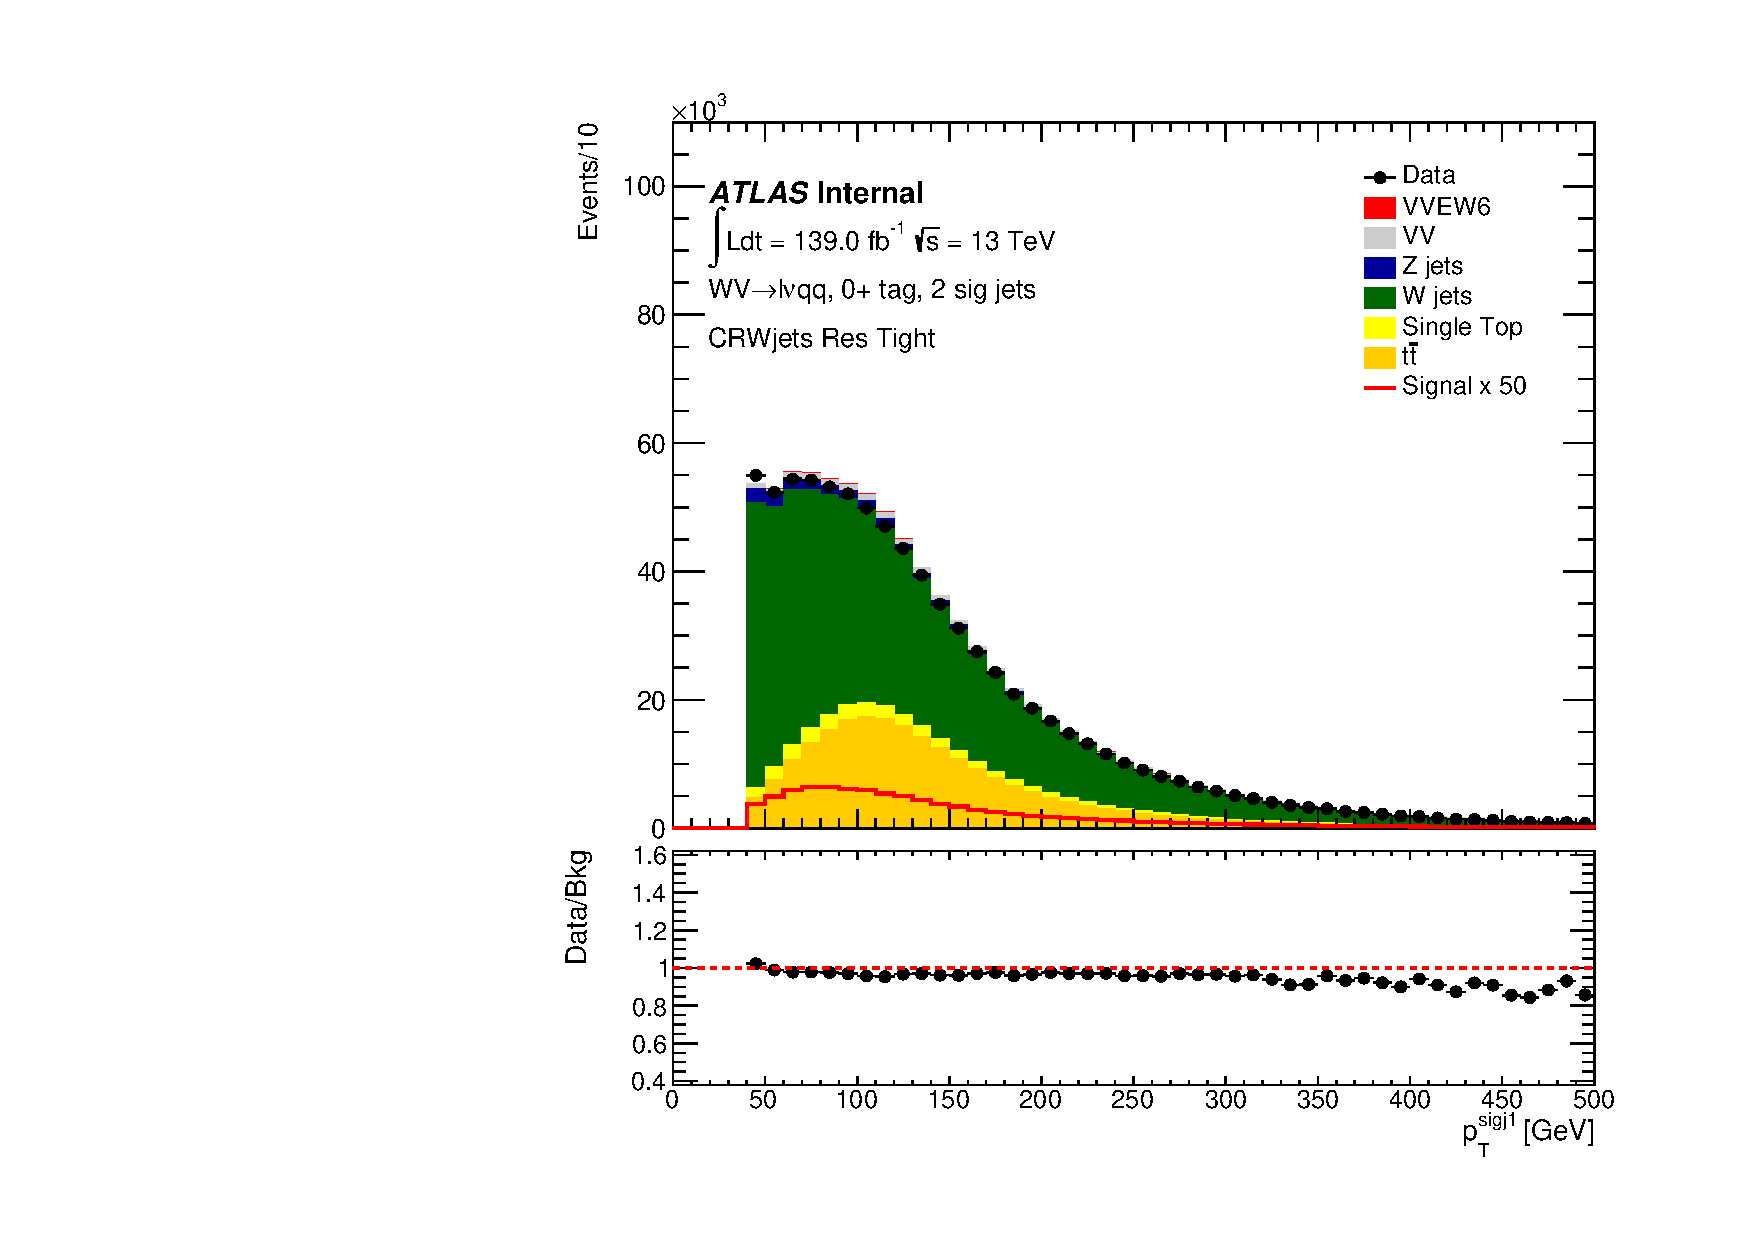
\includegraphics[width=0.3\textwidth]{figures/CRPlots/CRWjets_Res_Tight/stacked_plot_sigJ1_pt.pdf}}
    \subfloat[]{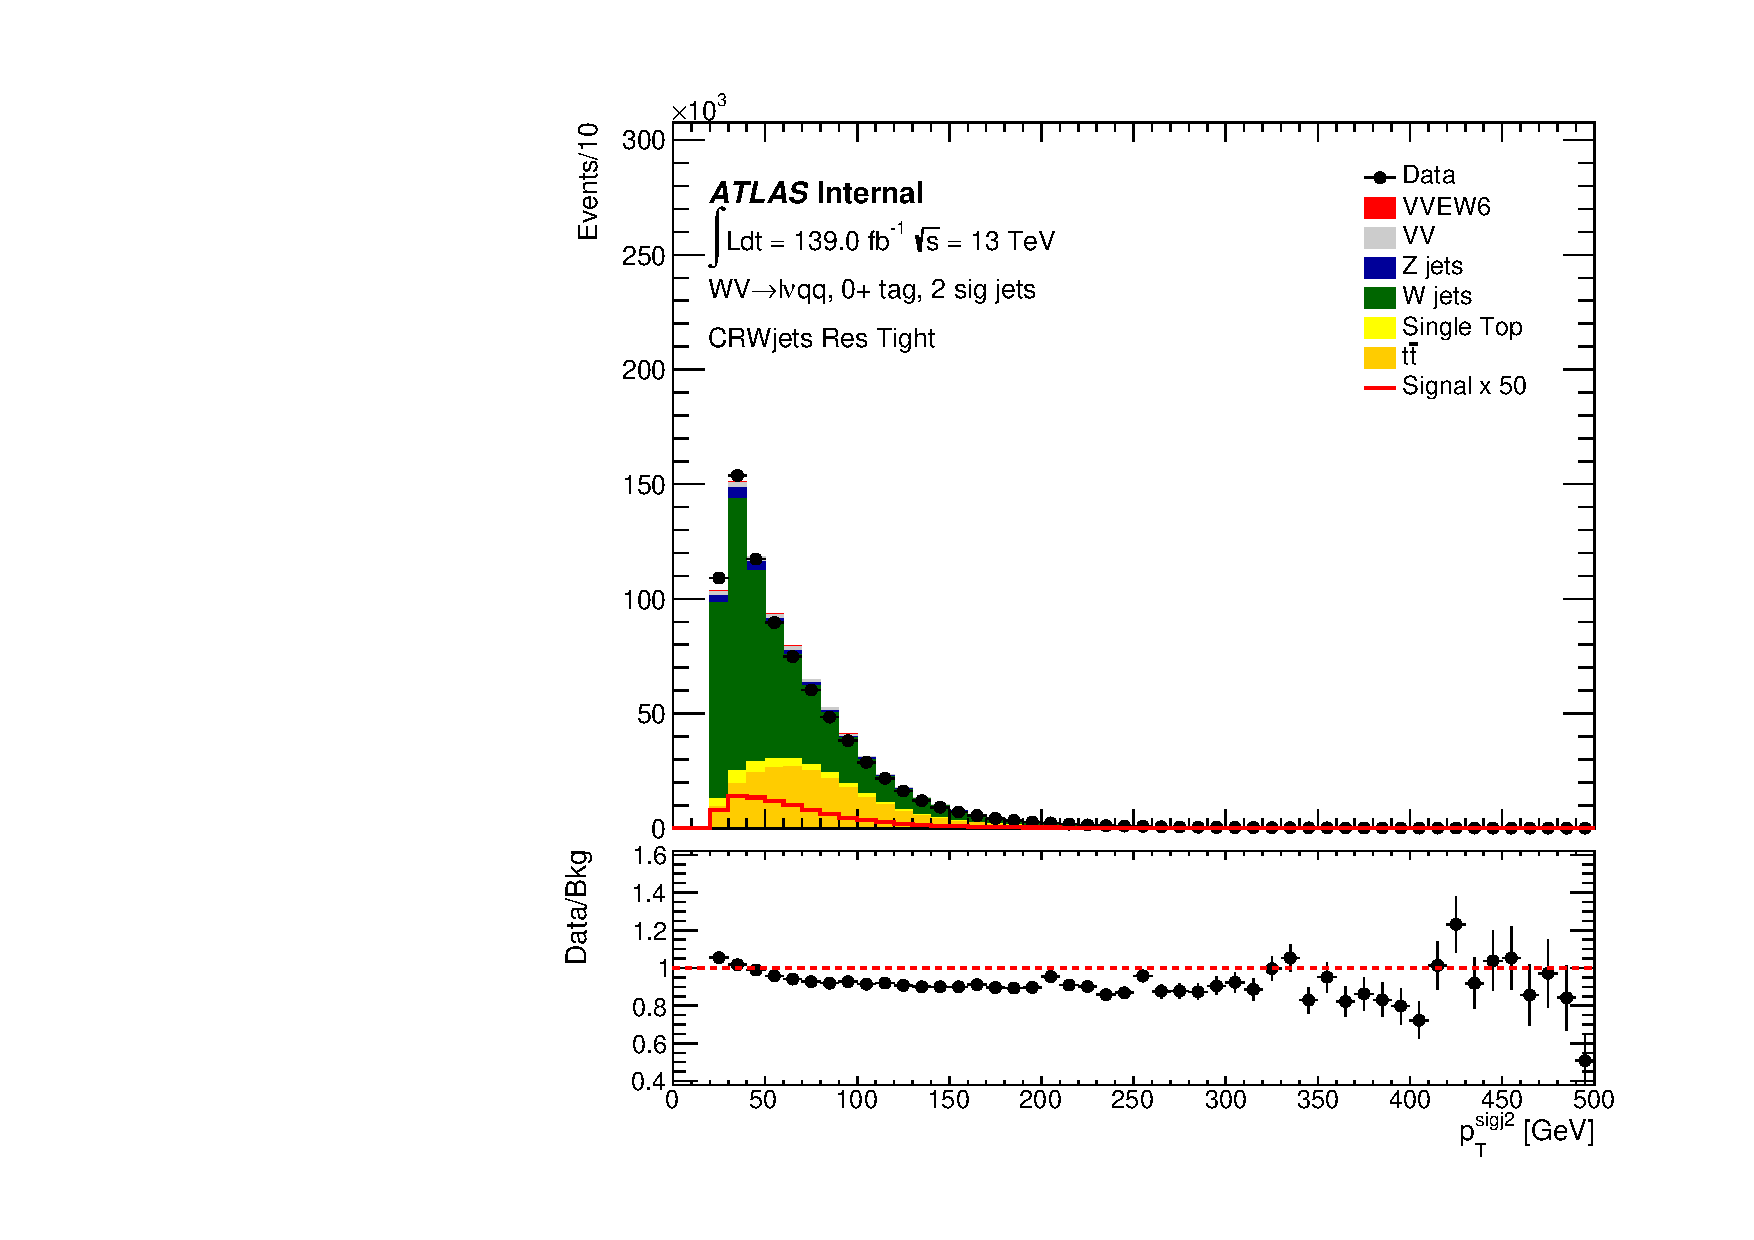
\includegraphics[width=0.3\textwidth]{figures/CRPlots/CRWjets_Res_Tight/stacked_plot_sigJ2_pt.pdf}} \\
    \subfloat[]{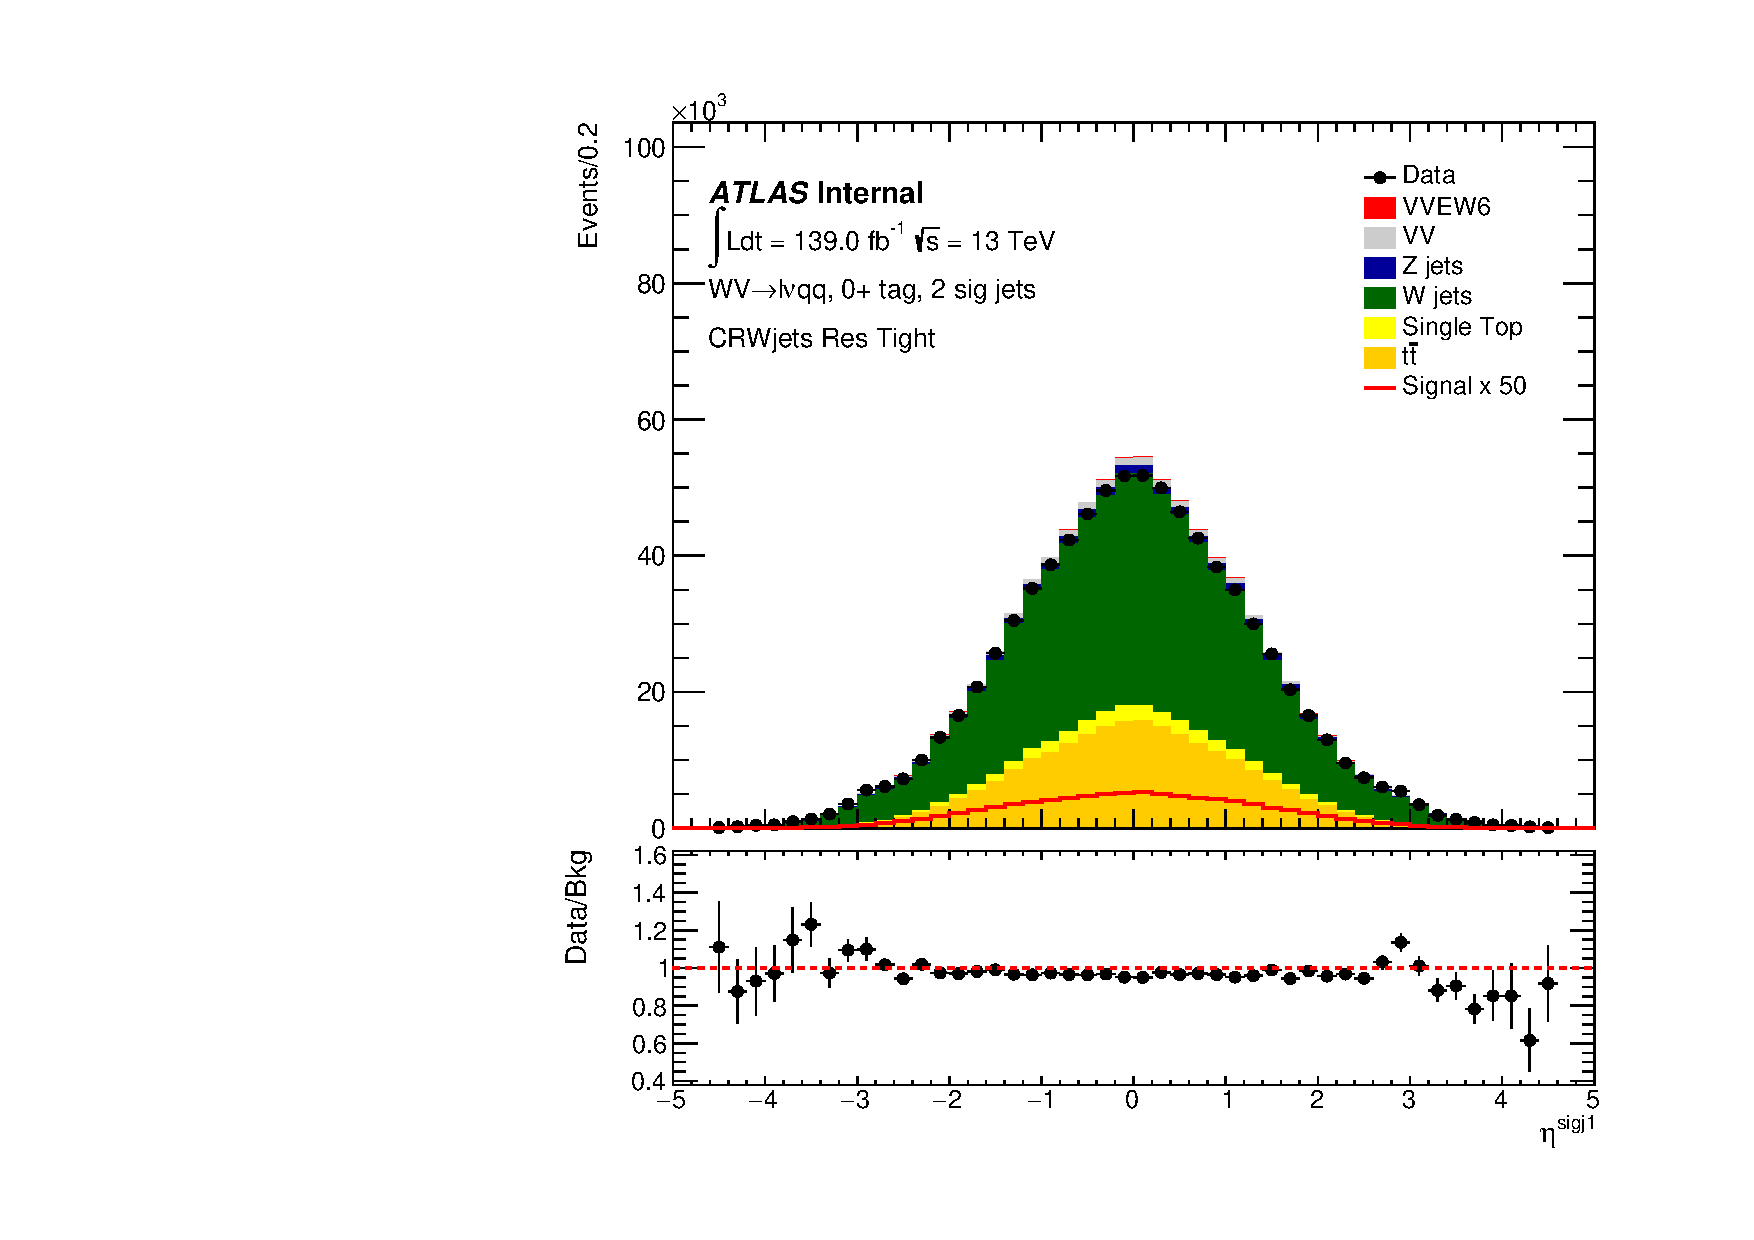
\includegraphics[width=0.3\textwidth]{figures/CRPlots/CRWjets_Res_Tight/stacked_plot_sigJ1_eta.pdf}}
    \subfloat[]{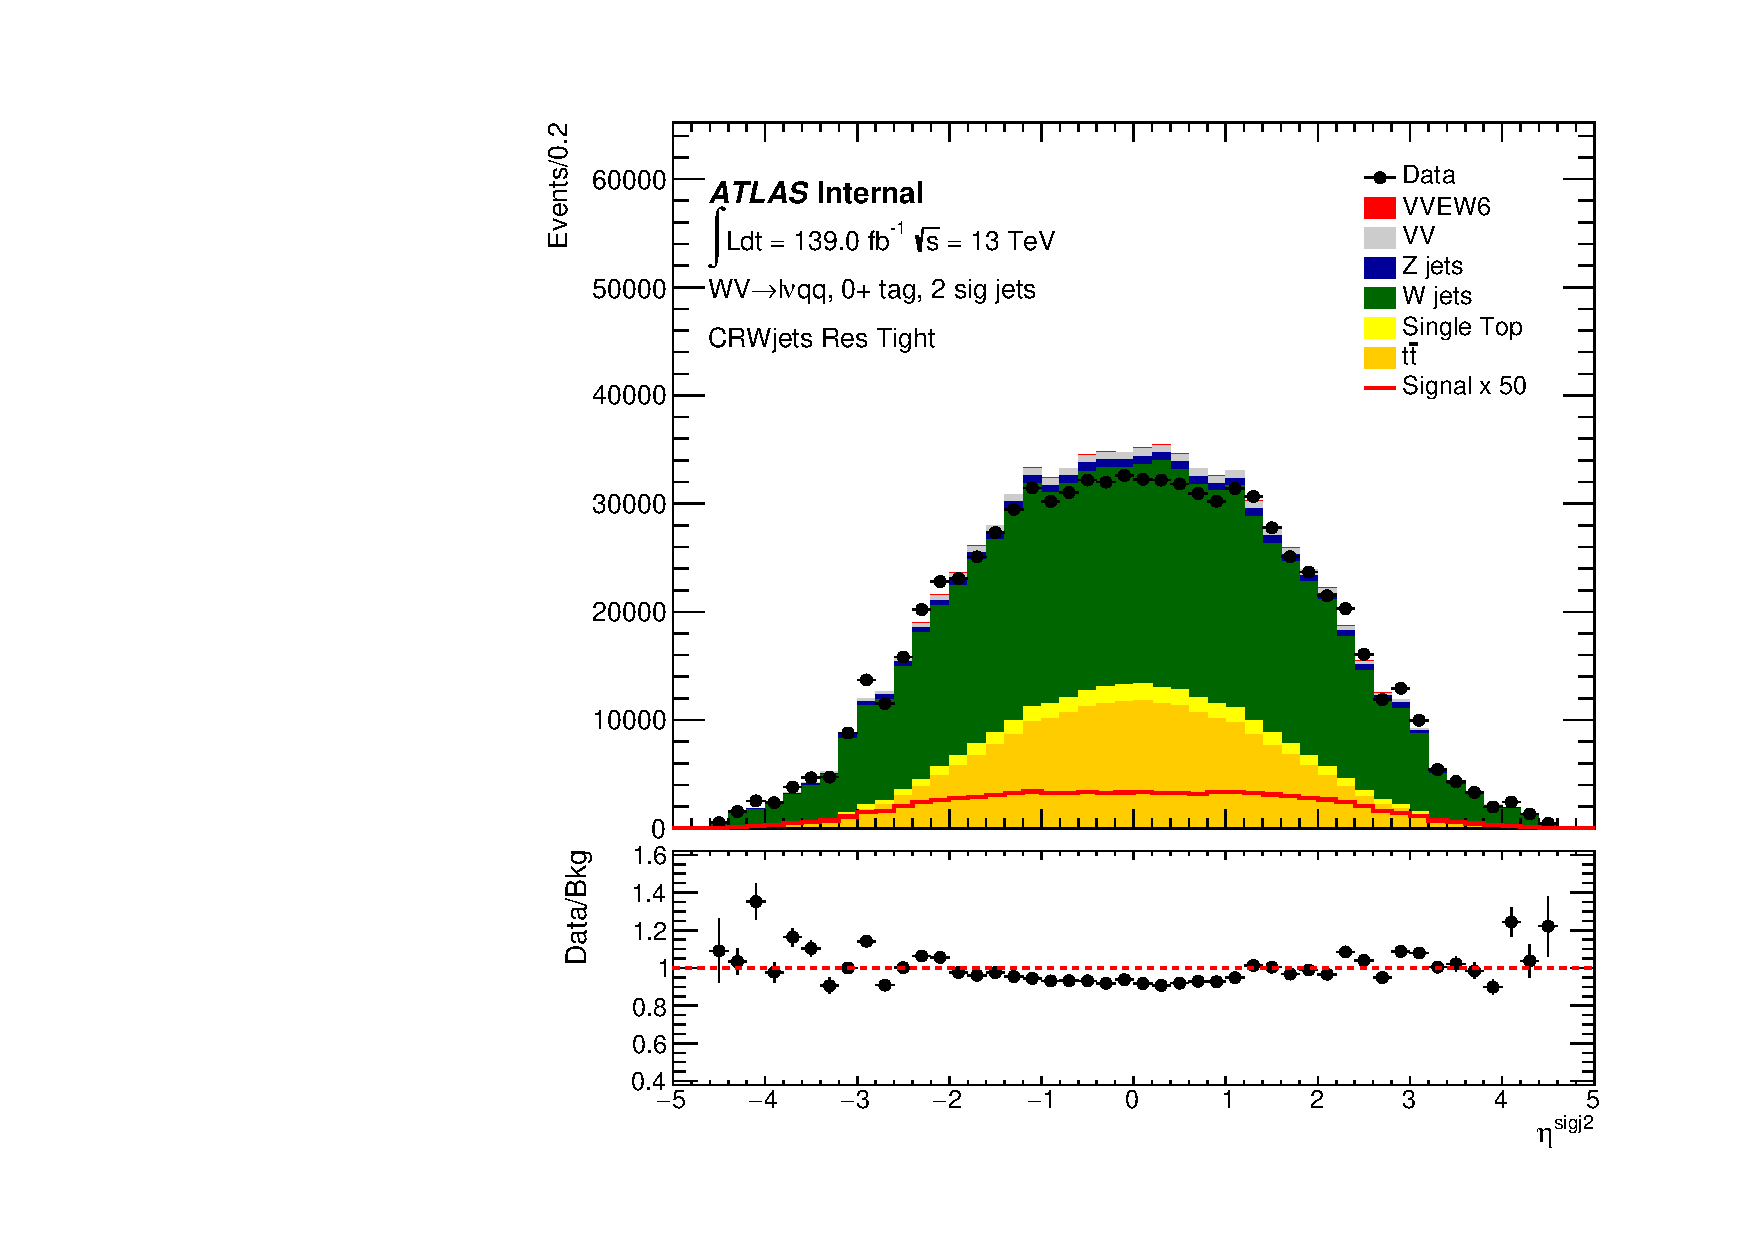
\includegraphics[width=0.3\textwidth]{figures/CRPlots/CRWjets_Res_Tight/stacked_plot_sigJ2_eta.pdf}} \\
    \subfloat[]{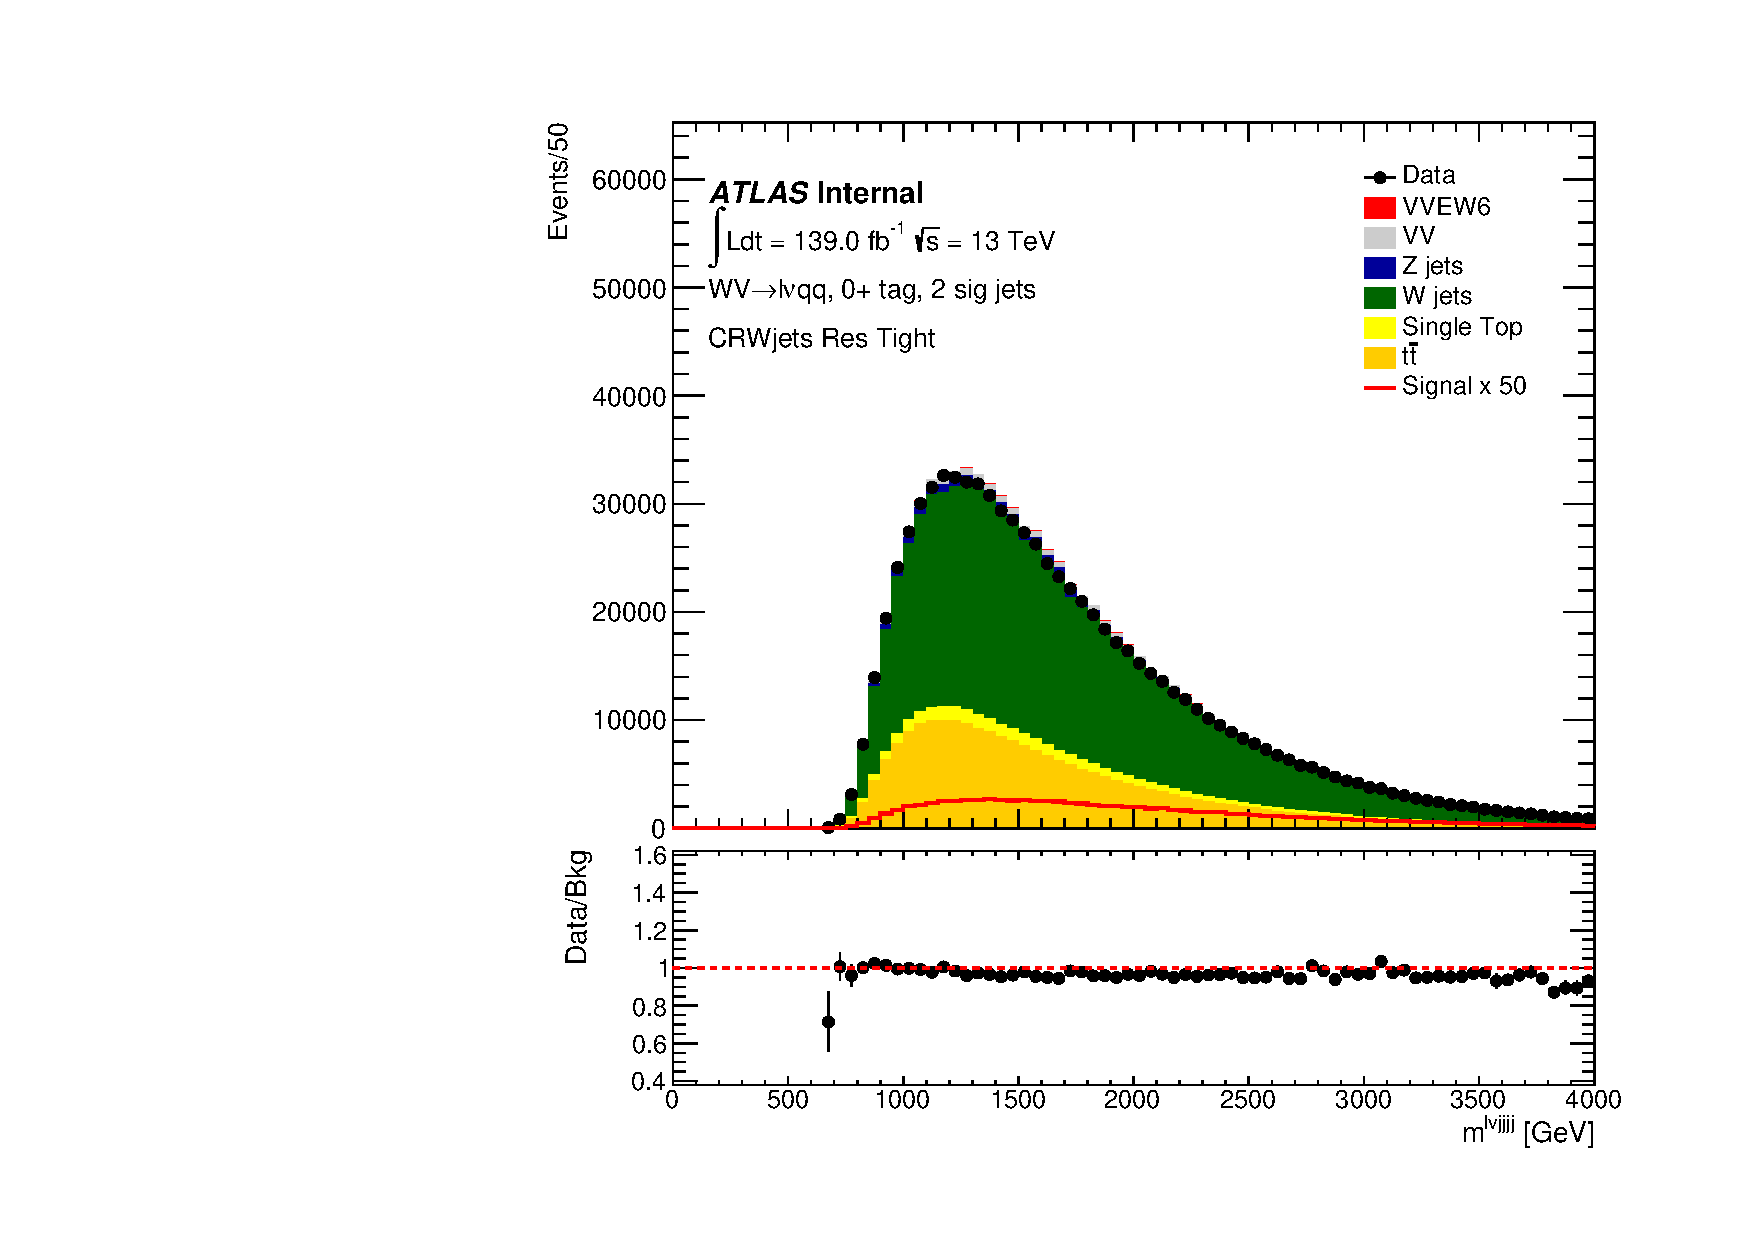
\includegraphics[width=0.3\textwidth]{figures/CRPlots/CRWjets_Res_Tight/stacked_plot_lvjjjjmass.pdf}}
    \subfloat[]{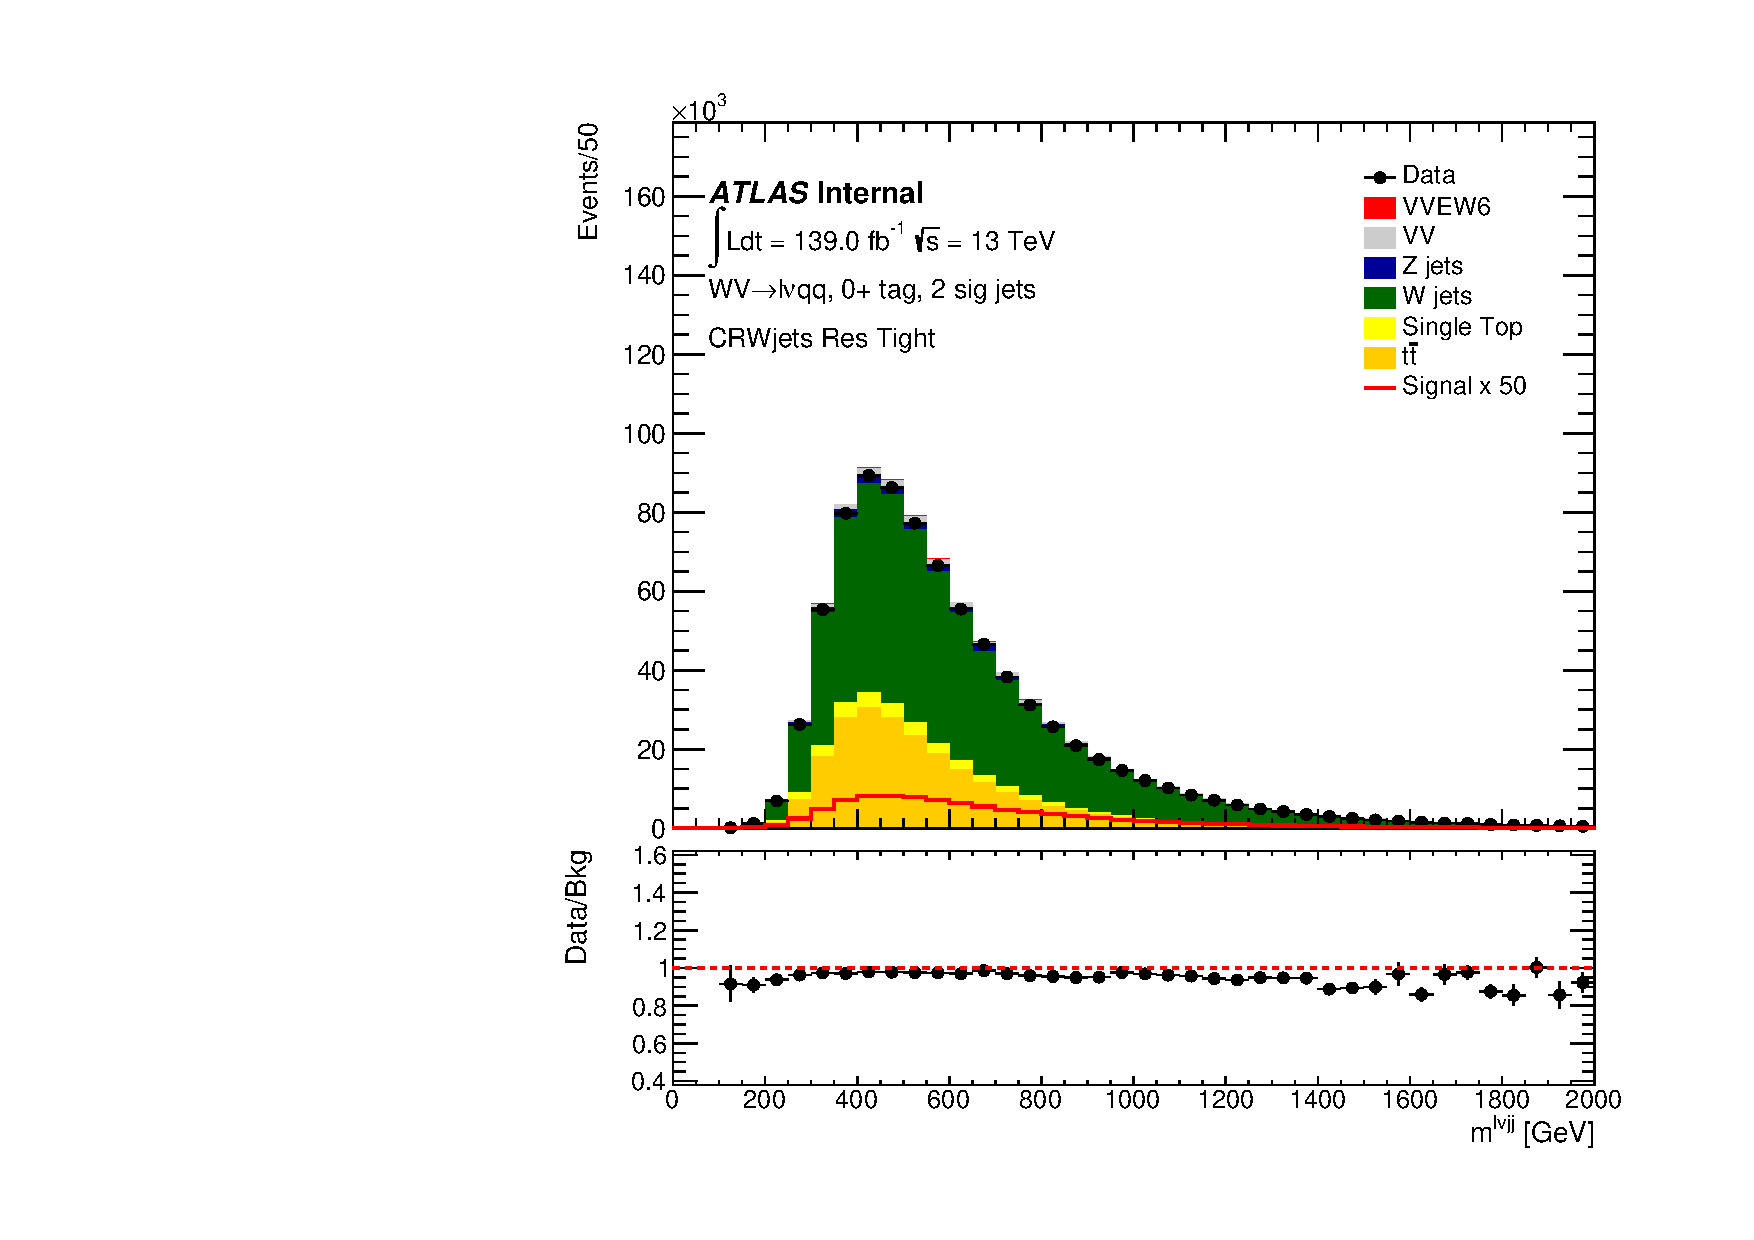
\includegraphics[width=0.3\textwidth]{figures/CRPlots/CRWjets_Res_Tight/stacked_plot_lvjjmass.pdf}}
    \subfloat[]{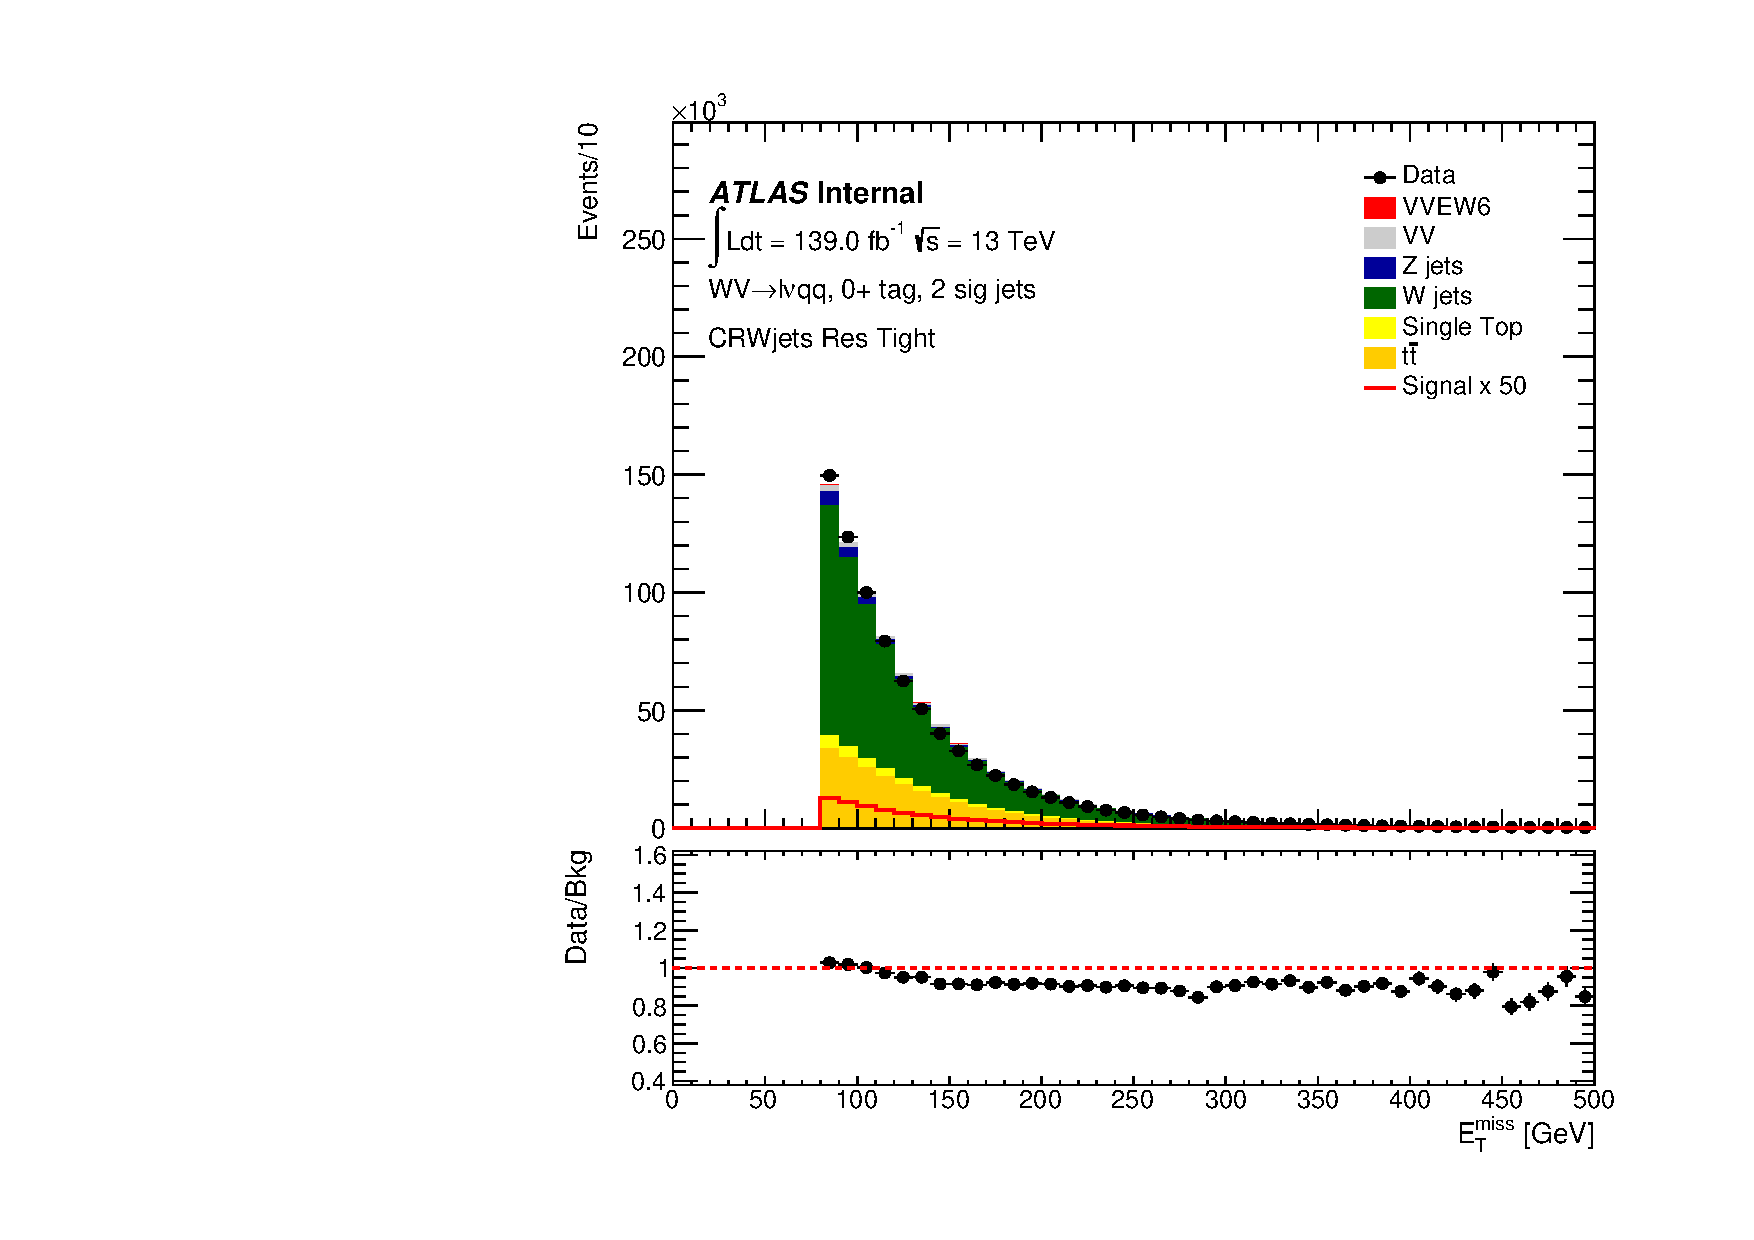
\includegraphics[width=0.3\textwidth]{figures/CRPlots/CRWjets_Res_Tight/stacked_plot_met.pdf}}  %%\\
%%    \subfloat[]{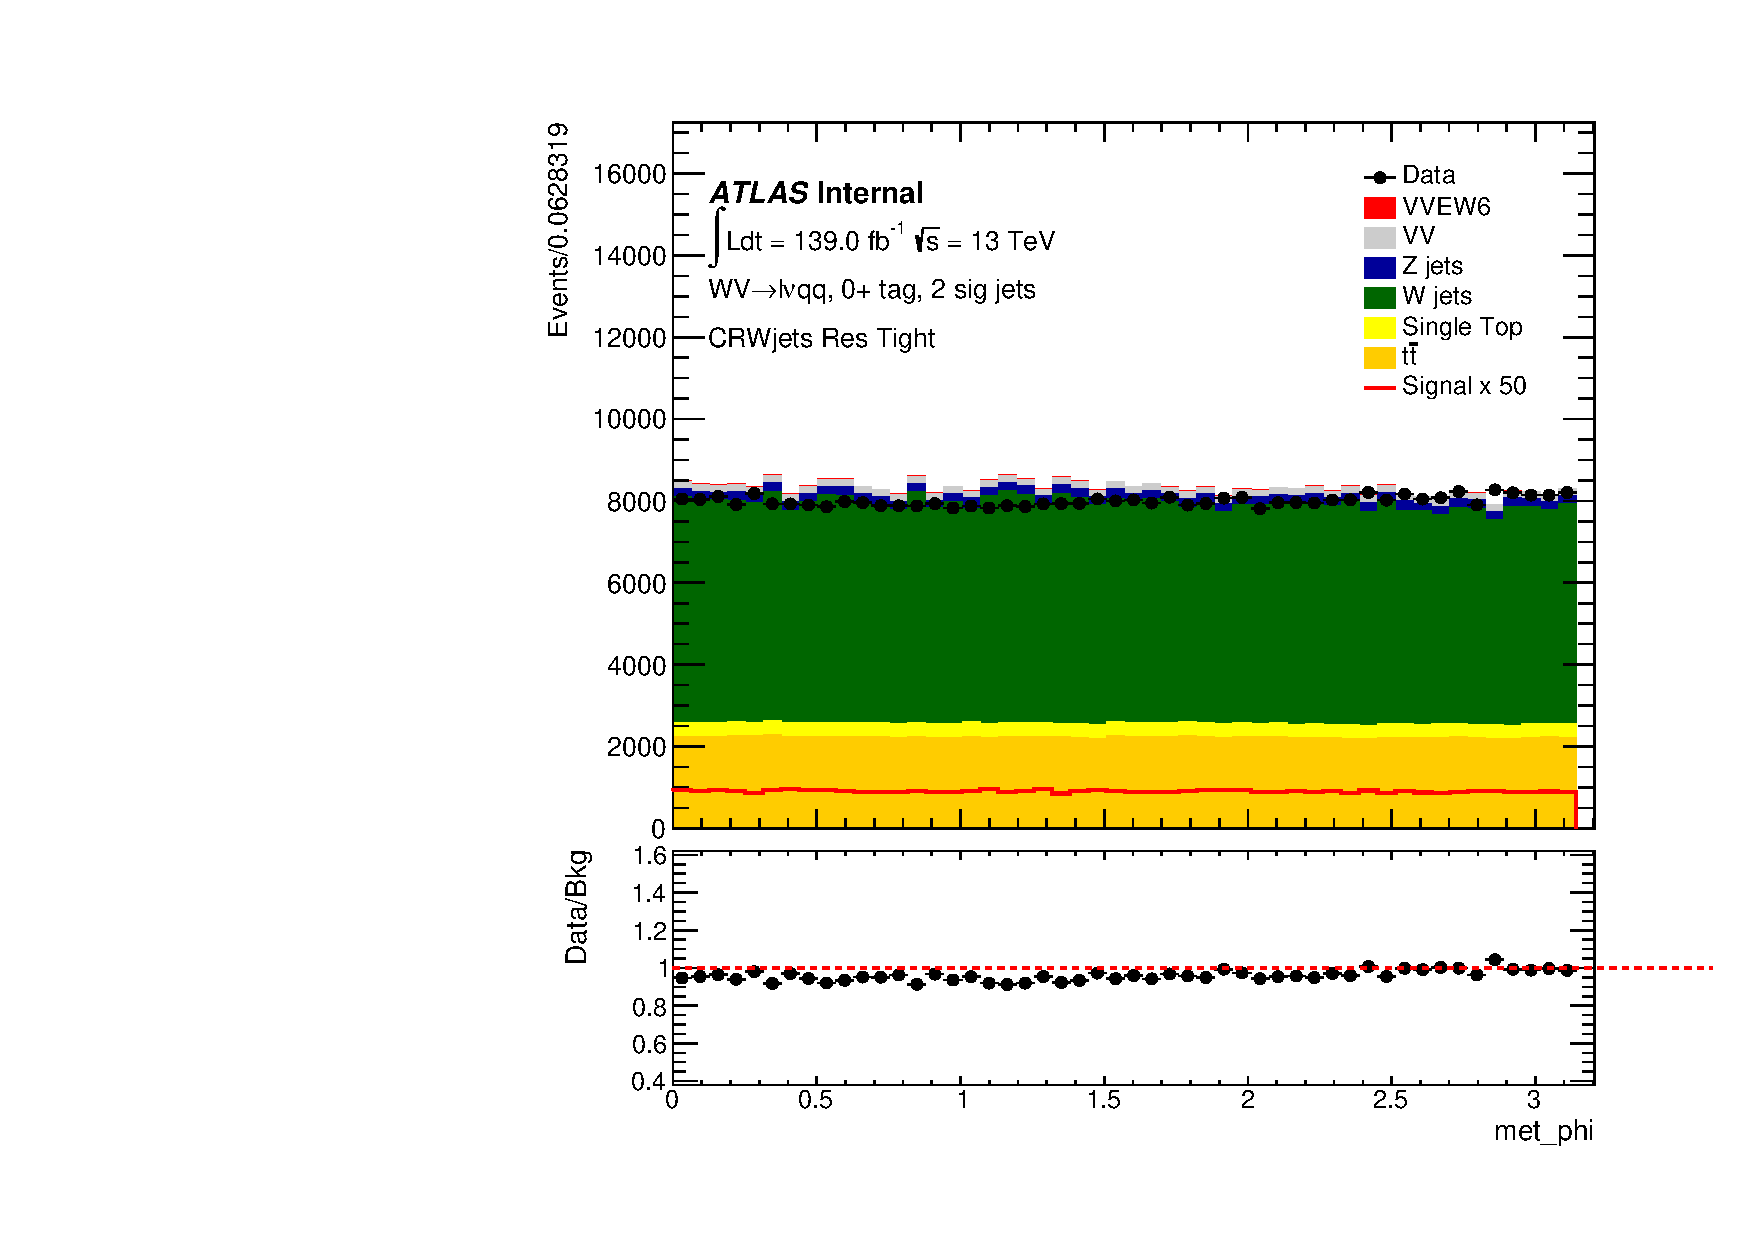
\includegraphics[width=0.3\textwidth]{figures/CRPlots/CRWjets_Res_Tight/stacked_plot_met_phi.pdf}}
%%    \subfloat[]{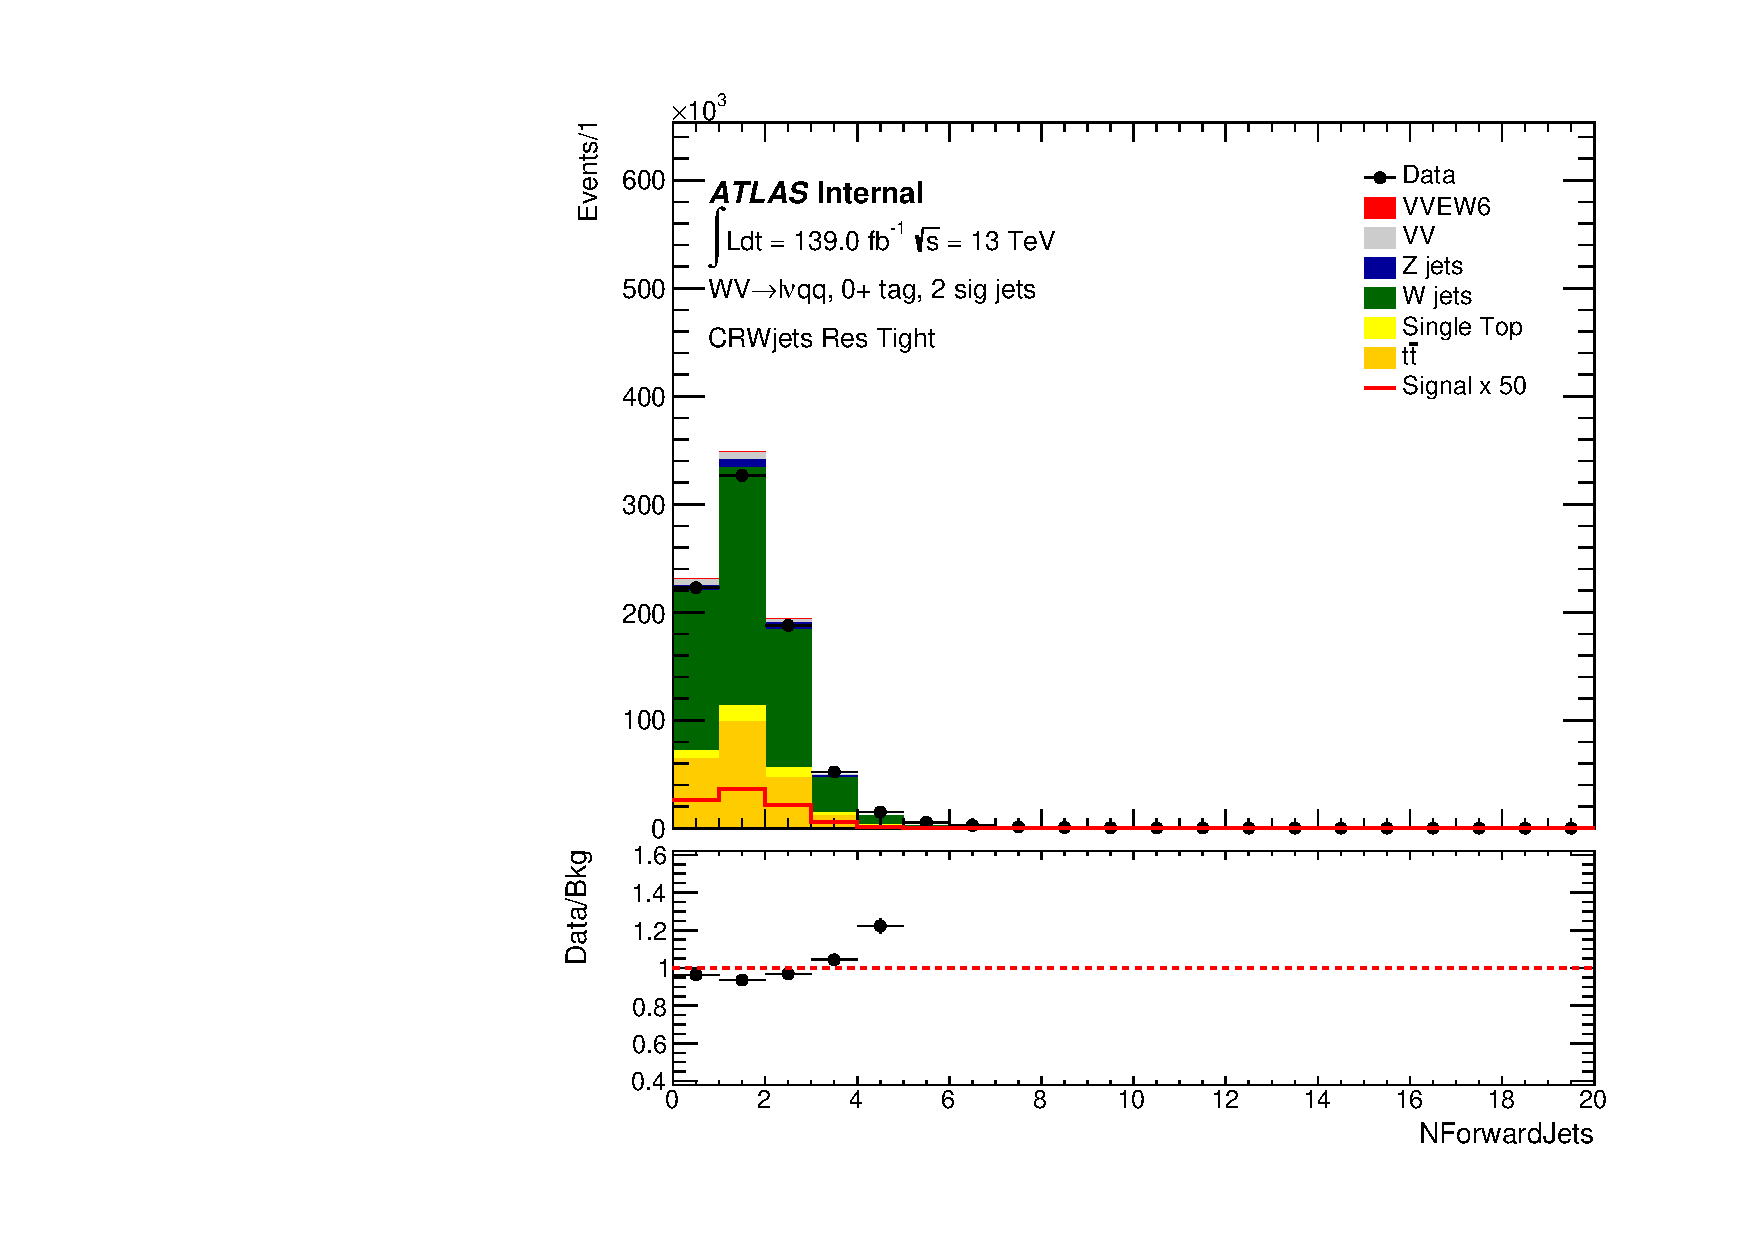
\includegraphics[width=0.3\textwidth]{figures/CRPlots/CRWjets_Res_Tight/stacked_plot_NForwardJets.pdf}}
    \caption{Data-MC checks for the resolved tight \Wjets control region in the \olep channel.}
    \label{fig:CRWjetResTightPlots1Lep2}
\end{figure}

\begin{figure}[ht]
    \centering
    \subfloat[]{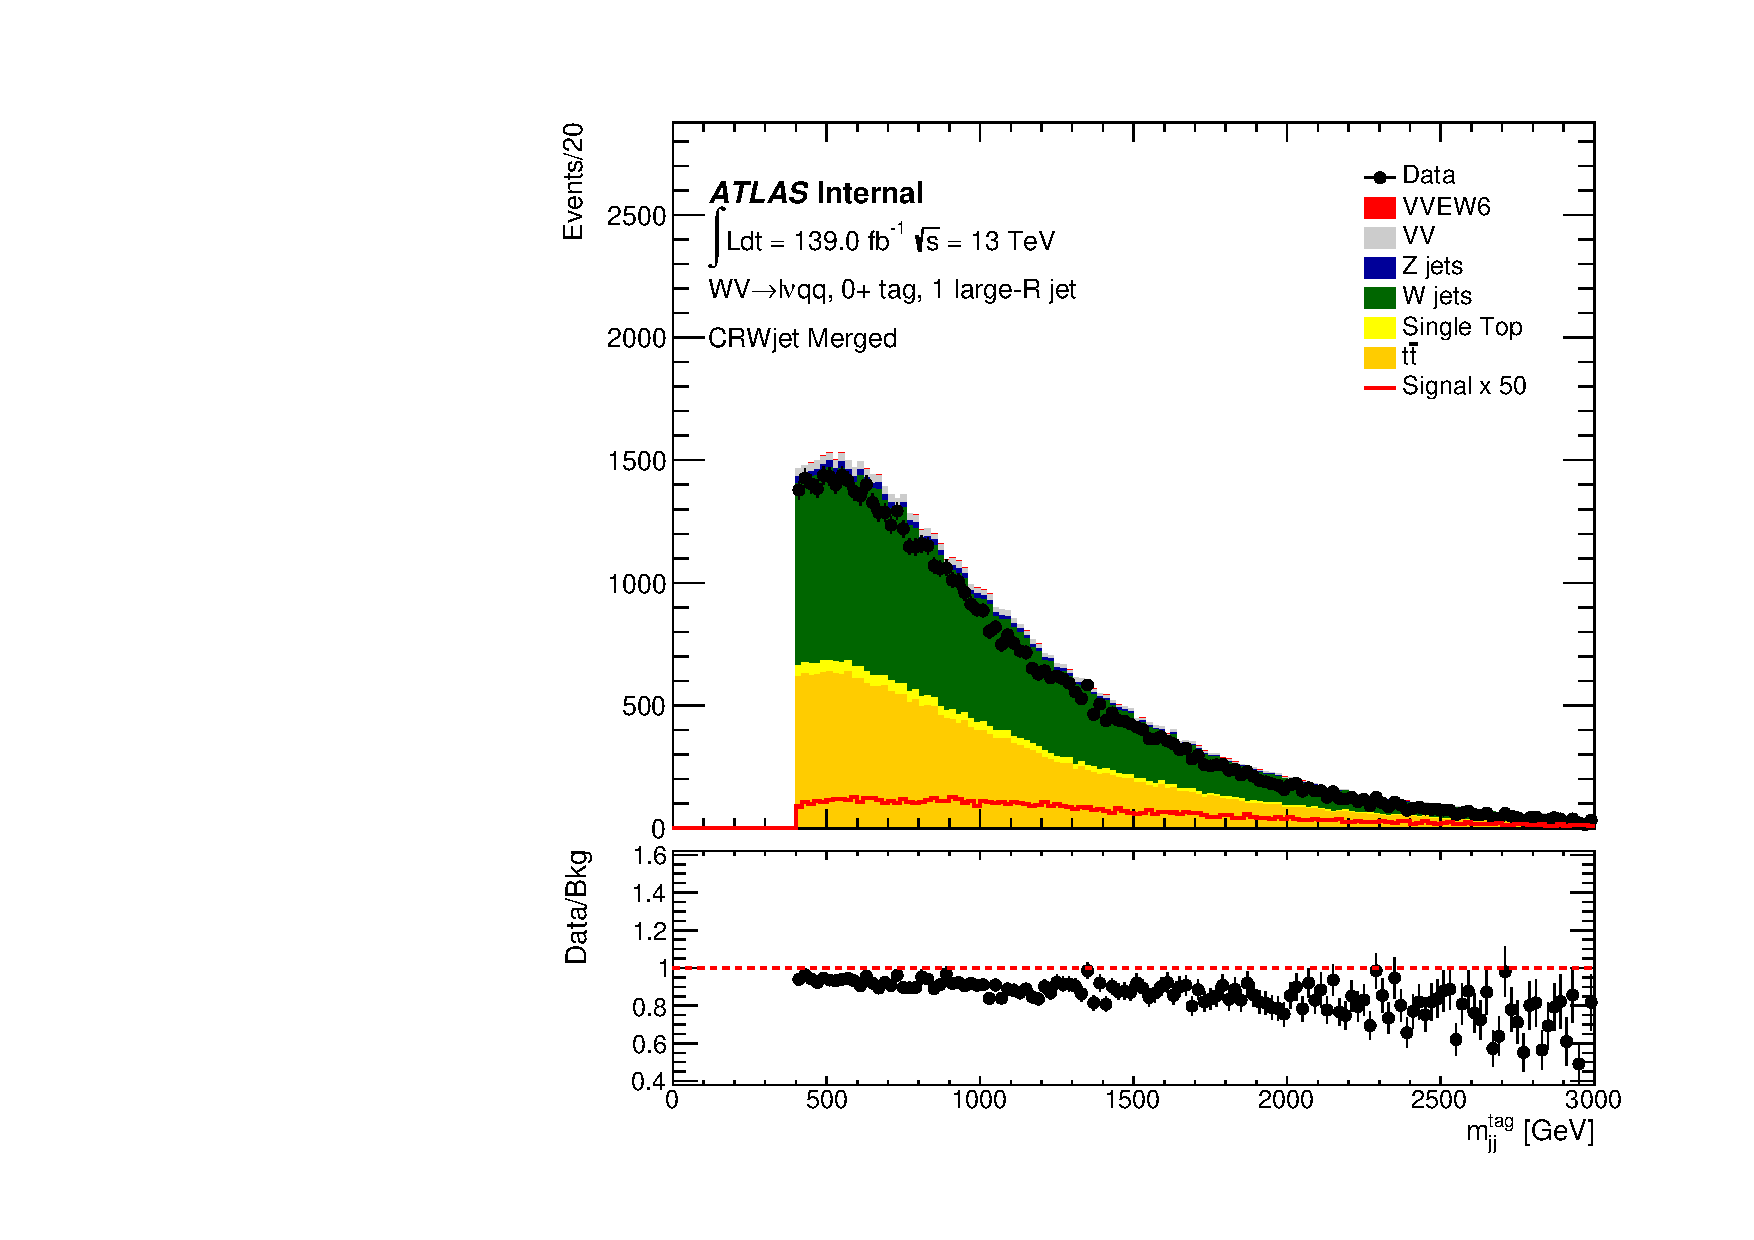
\includegraphics[width=0.3\textwidth]{figures/CRPlots/CRWjets100/stacked_plot_merged_tagMjj.pdf}}
    \subfloat[]{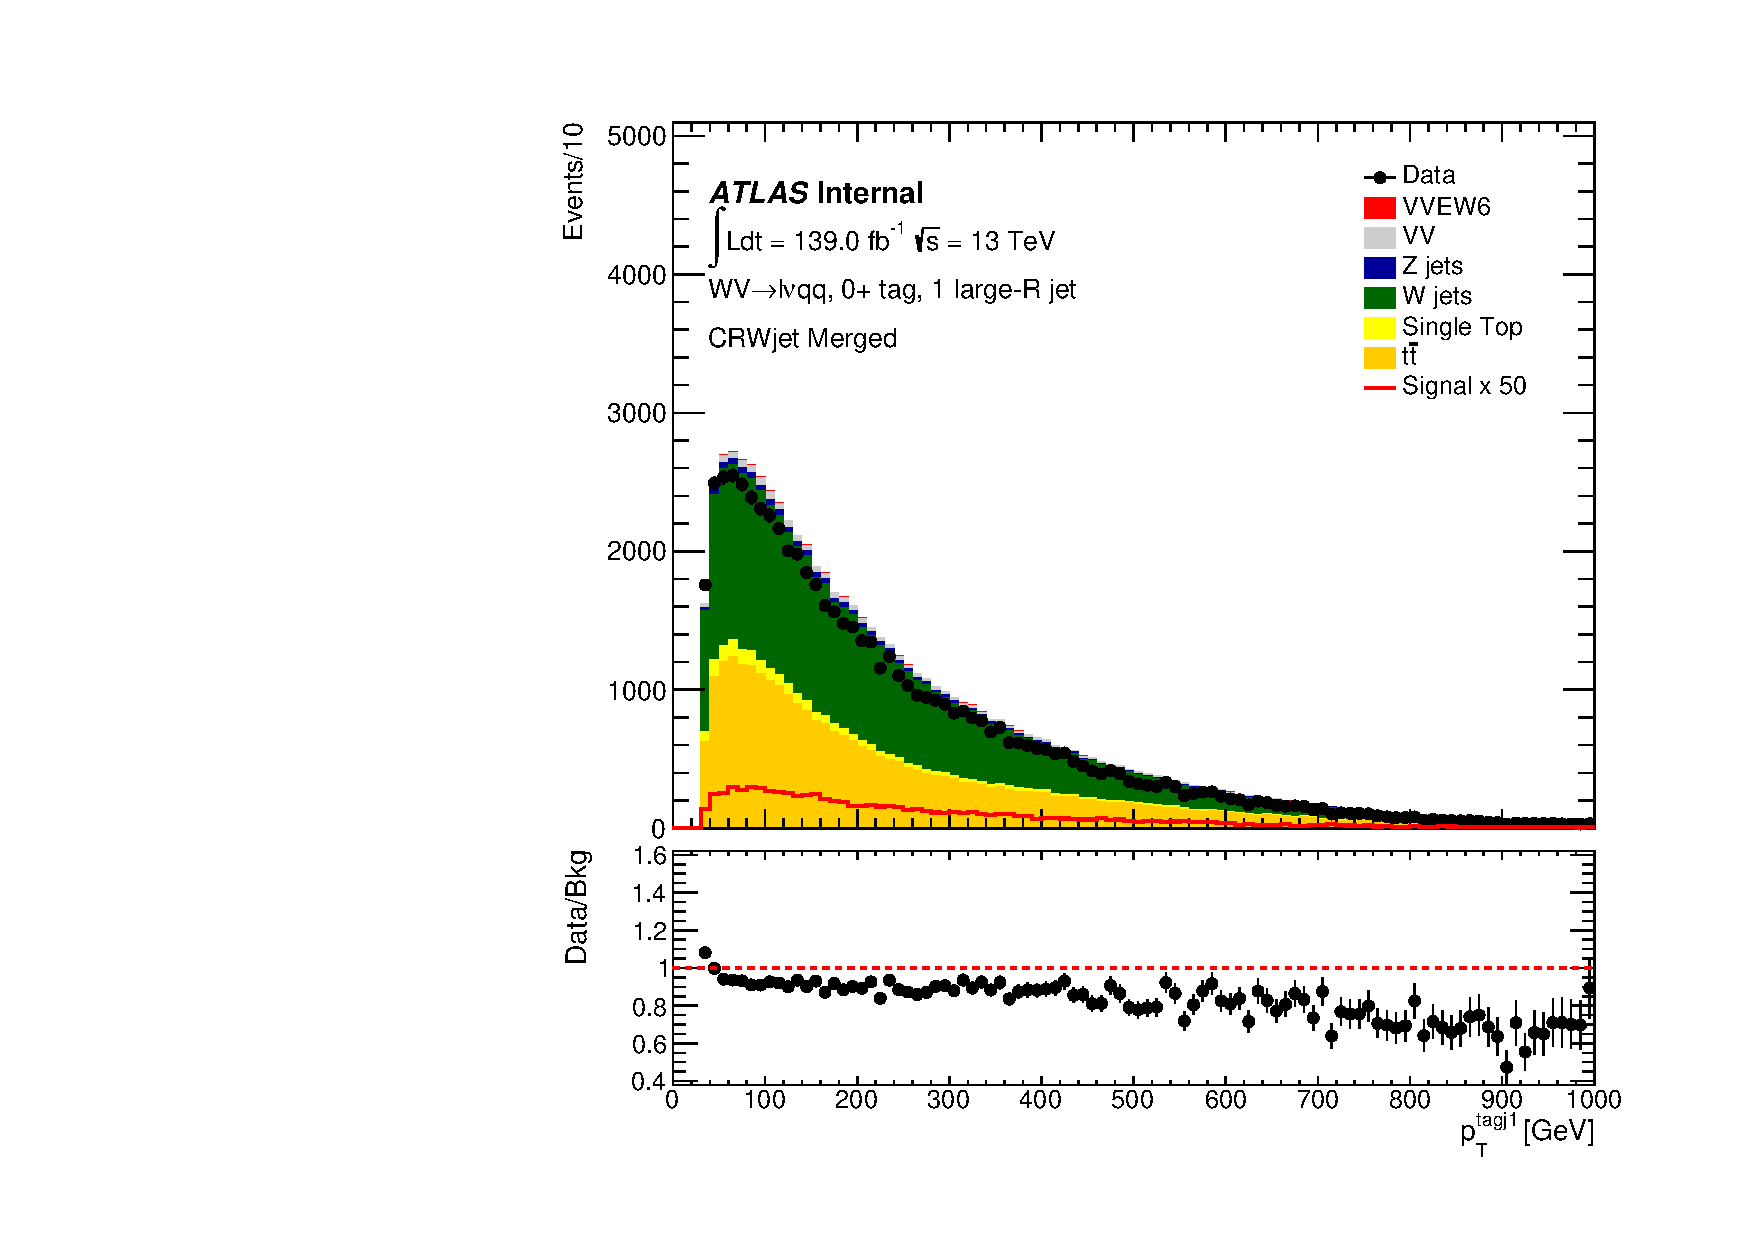
\includegraphics[width=0.3\textwidth]{figures/CRPlots/CRWjets100/stacked_plot_merged_tagJ1_pt.pdf}}
    \subfloat[]{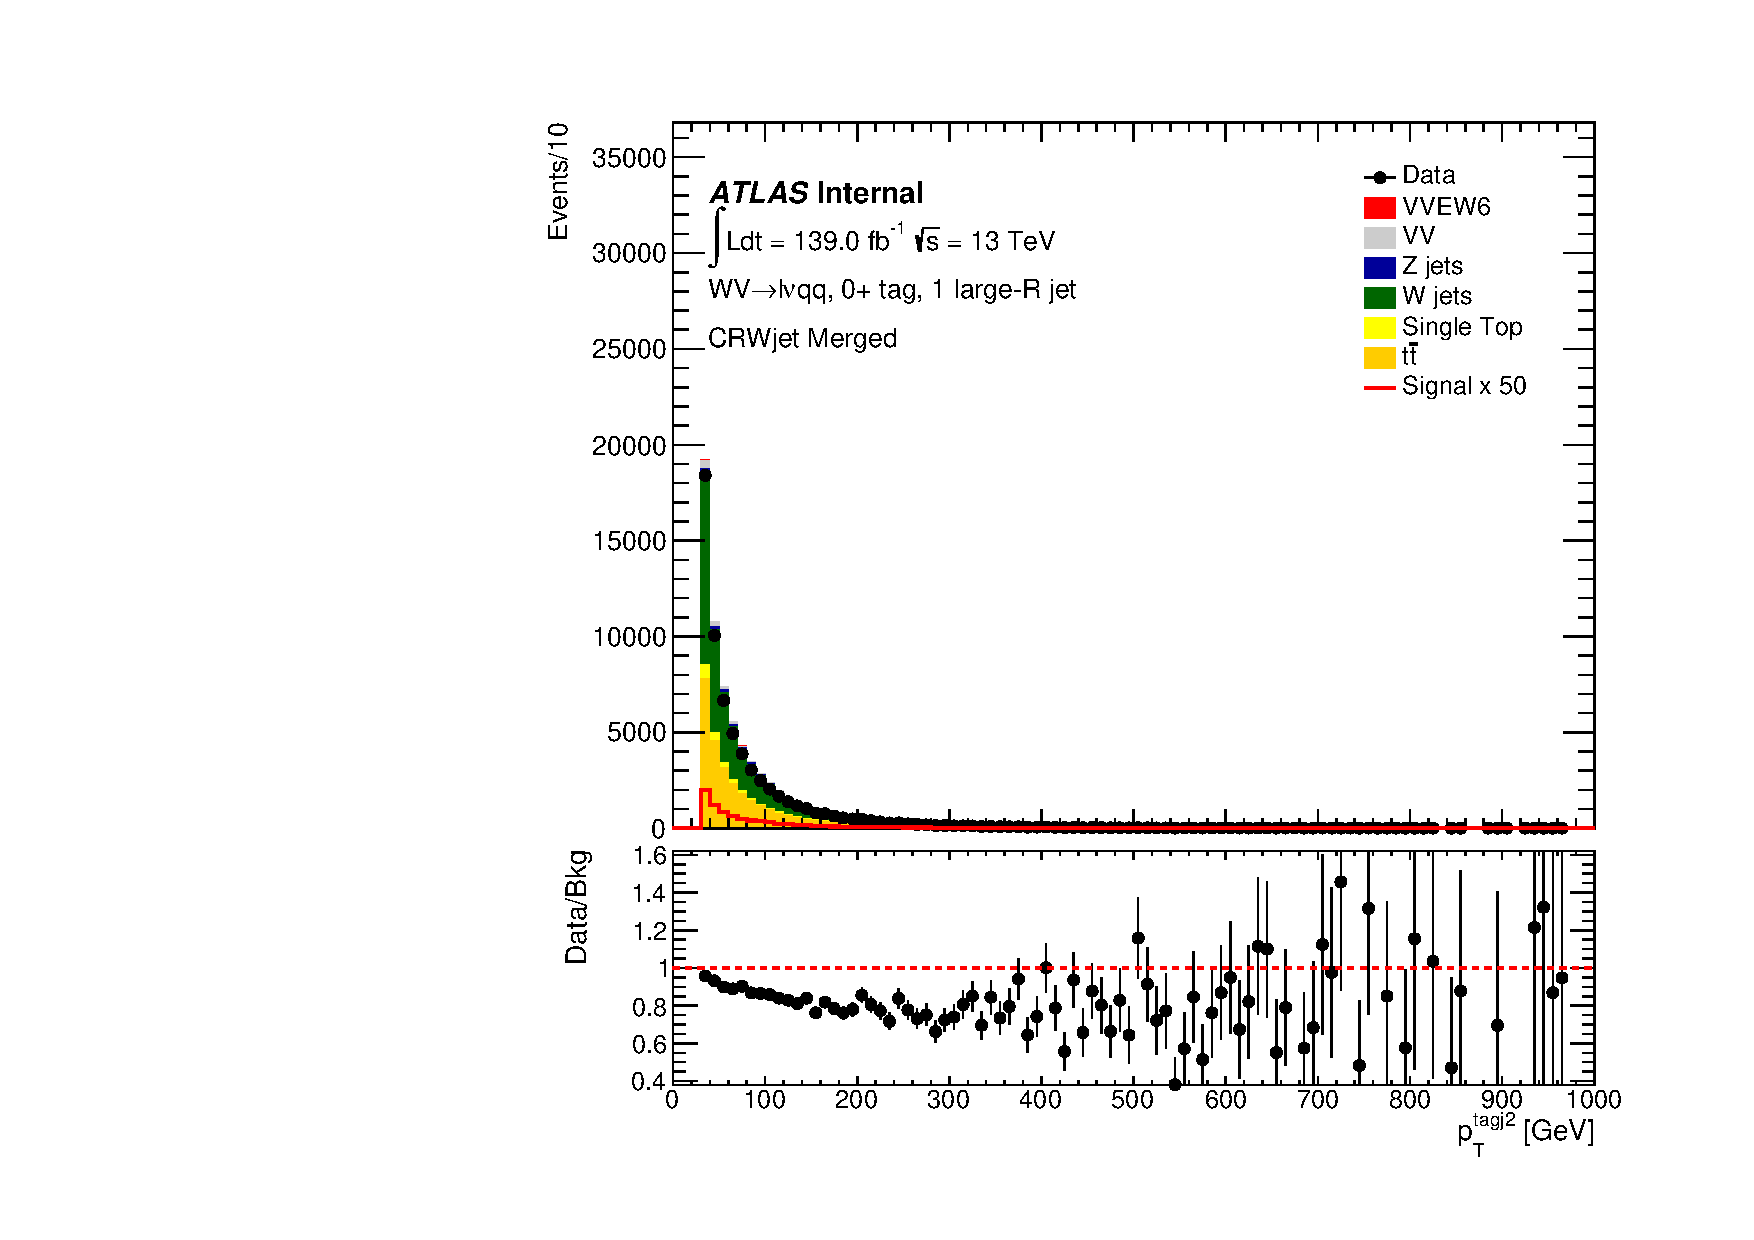
\includegraphics[width=0.3\textwidth]{figures/CRPlots/CRWjets100/stacked_plot_merged_tagJ2_pt.pdf}} \\
    \subfloat[]{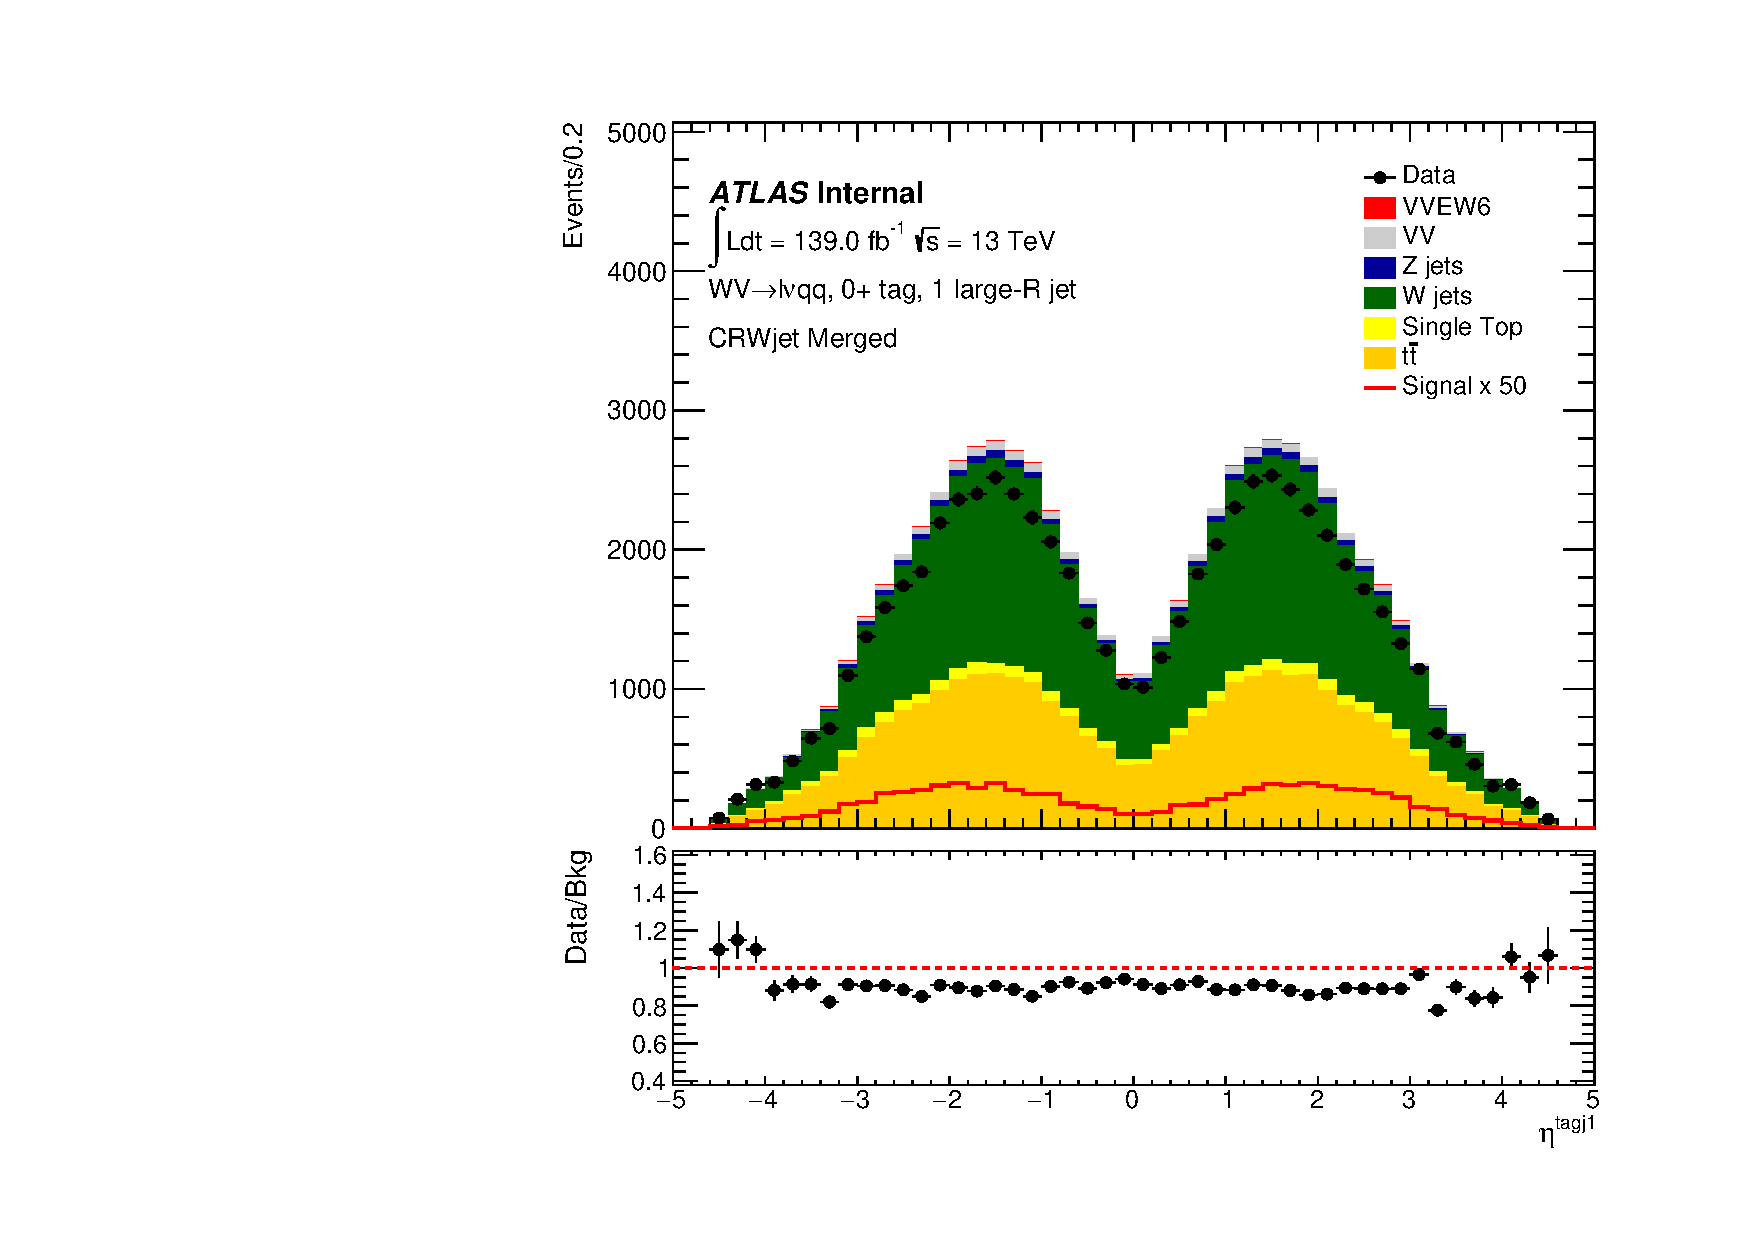
\includegraphics[width=0.3\textwidth]{figures/CRPlots/CRWjets100/stacked_plot_merged_tagJ1_eta.pdf}}
    \subfloat[]{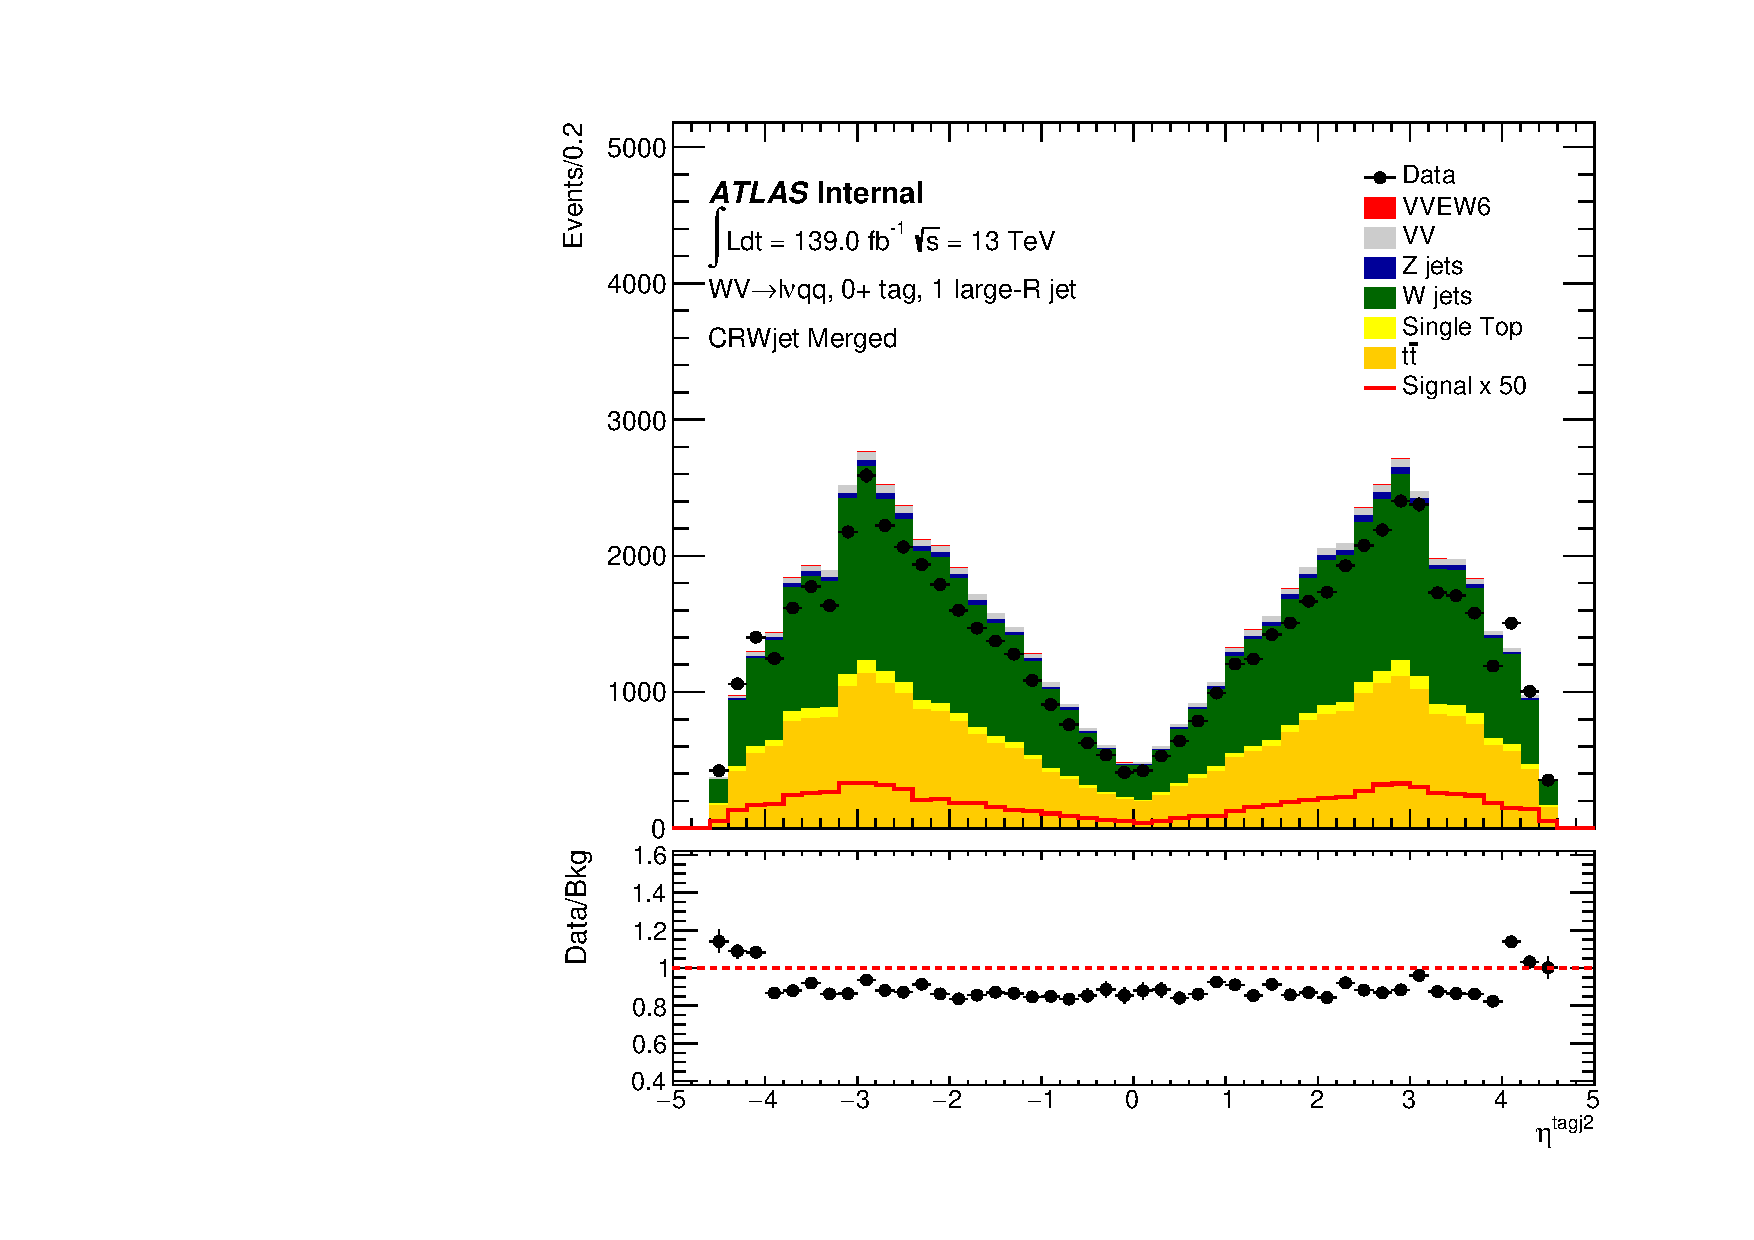
\includegraphics[width=0.3\textwidth]{figures/CRPlots/CRWjets100/stacked_plot_merged_tagJ2_eta.pdf}}
    \subfloat[]{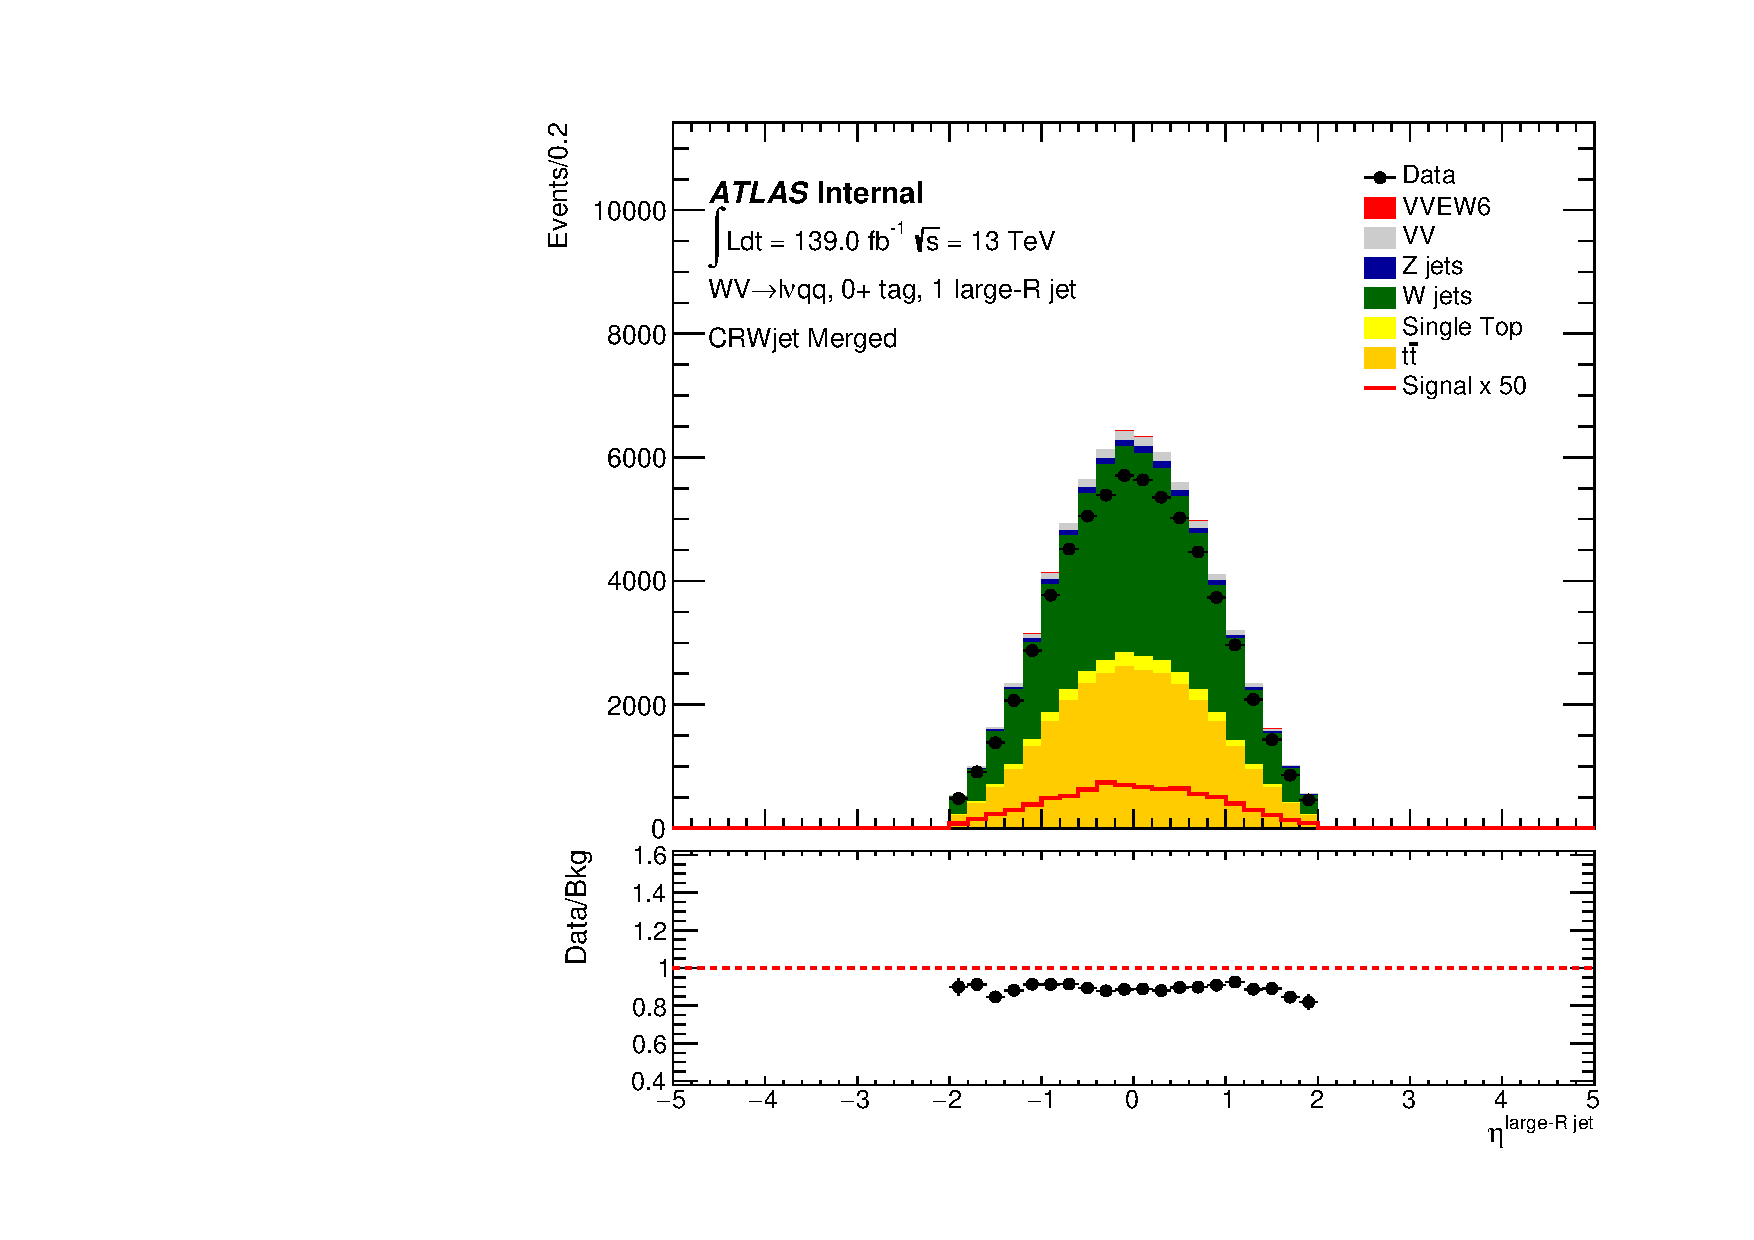
\includegraphics[width=0.3\textwidth]{figures/CRPlots/CRWjets100/stacked_plot_fatJ_eta.pdf}} \\
    \subfloat[]{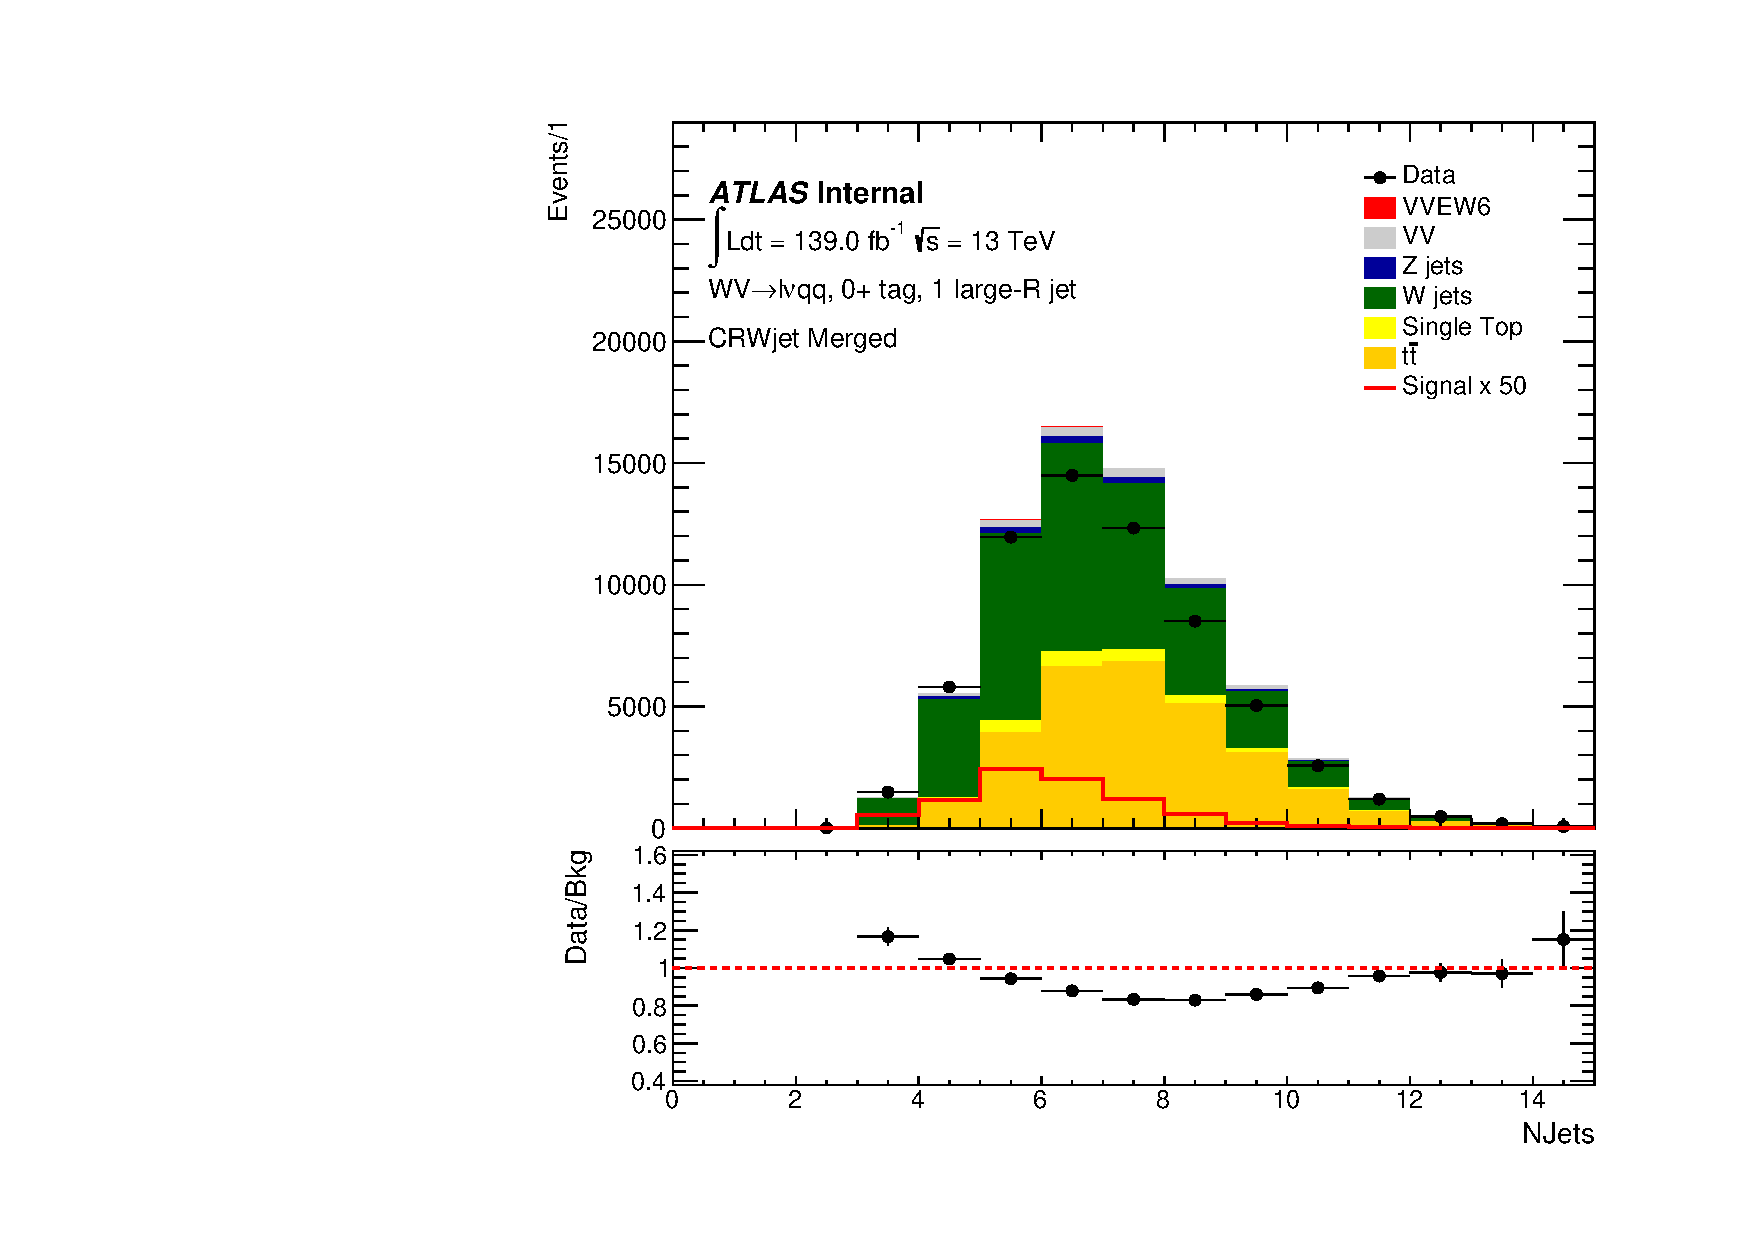
\includegraphics[width=0.3\textwidth]{figures/CRPlots/CRWjets100/stacked_plot_NJets.pdf}}
    \subfloat[]{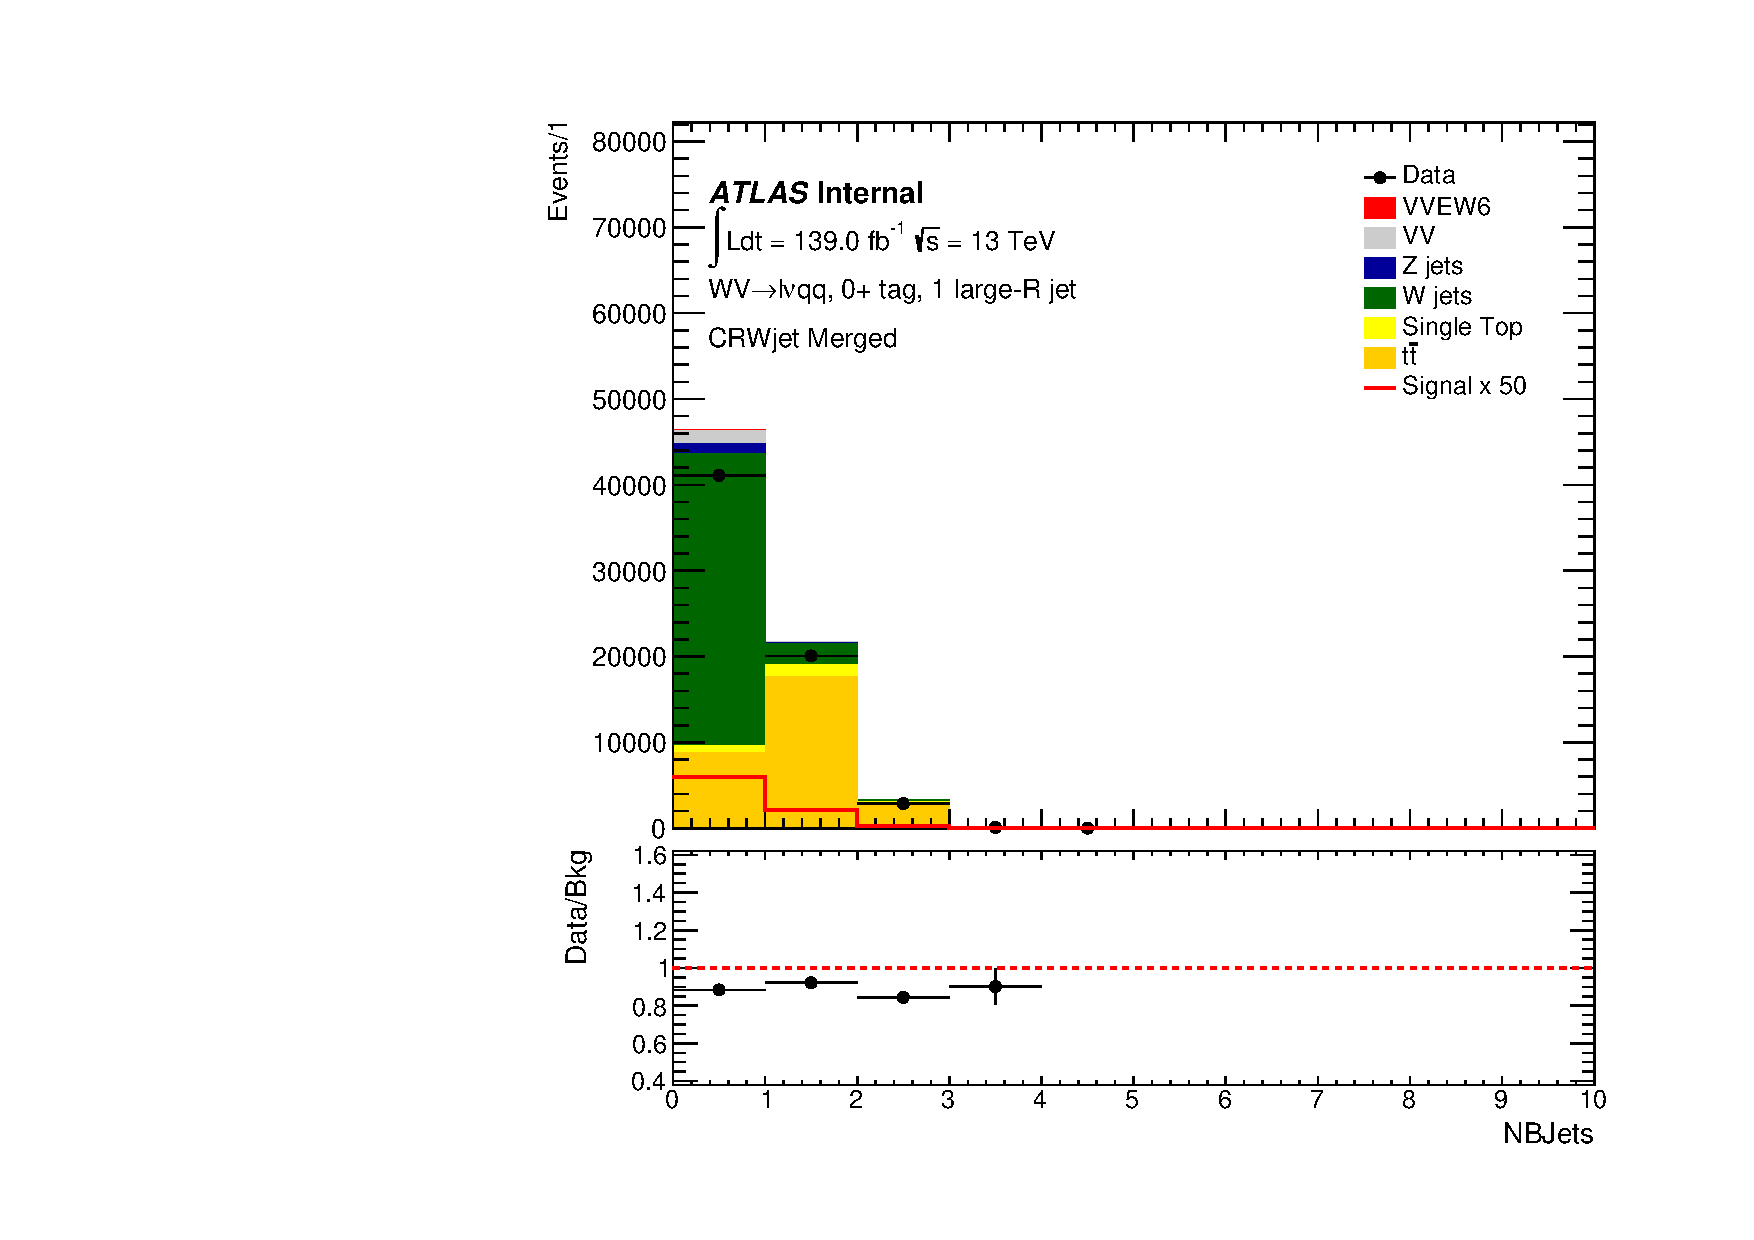
\includegraphics[width=0.3\textwidth]{figures/CRPlots/CRWjets100/stacked_plot_NBJets.pdf}}
    \subfloat[]{\includegraphics[width=0.3\textwidth]{figures/CRPlots/CRWjets100/stacked_plot_lep_pt.pdf}}  \\
    \subfloat[]{\includegraphics[width=0.3\textwidth]{figures/CRPlots/CRWjets100/stacked_plot_fatJ_m.pdf}}
    \subfloat[]{\includegraphics[width=0.3\textwidth]{figures/CRPlots/CRWjets100/stacked_plot_fatJ_pt.pdf}}
    \subfloat[]{\includegraphics[width=0.3\textwidth]{figures/CRPlots/CRWjets100/stacked_plot_fatJ_D2.pdf}}
    \caption{Data-MC checks for the merged \Wjets control region in the \olep channel.}
    \label{fig:CRWjetMerPlots1Lep}
\end{figure}

\begin{figure}[ht]
    \centering
    \subfloat[]{\includegraphics[width=0.3\textwidth]{figures/CRPlots/CRWjets100/stacked_plot_W_m.pdf}}
    \subfloat[]{\includegraphics[width=0.3\textwidth]{figures/CRPlots/CRWjets100/stacked_plot_W_pt.pdf}}
    \subfloat[]{\includegraphics[width=0.3\textwidth]{figures/CRPlots/CRWjets100/stacked_plot_W_eta.pdf}} \\
    \subfloat[]{\includegraphics[width=0.3\textwidth]{figures/CRPlots/CRWjets100/stacked_plot_merged_tagJdEta.pdf}}
    \subfloat[]{\includegraphics[width=0.3\textwidth]{figures/CRPlots/CRWjets100/stacked_plot_fatJ_dRj1.pdf}}
    \subfloat[]{\includegraphics[width=0.3\textwidth]{figures/CRPlots/CRWjets100/stacked_plot_fatJ_dRj2.pdf}} \\
    \subfloat[]{\includegraphics[width=0.3\textwidth]{figures/CRPlots/CRWjets100/stacked_plot_lvJjjmass.pdf}}
    \subfloat[]{\includegraphics[width=0.3\textwidth]{figures/CRPlots/CRWjets100/stacked_plot_lvJmass.pdf}} \\
    \caption{Data-MC checks for the merged \Wjets control region in the \olep channel.}
    \label{fig:CRWjetMerPlots1Lep2}
\end{figure}

